%include header with all settings
\documentclass[
a4paper,							% alle weiteren Papierformat einstellbar
%landscape,						% Querformat
12pt,						  		% Schriftgrˆfle (12pt, 11pt (Standard))
BCOR1cm,							% Bindekorrektur, bspw. 1 cm
DIV=calc,							% f¸hrt die Satzspiegelberechnung neu aus scrguide 2.4
twoside, 						% zweiseitig twoside/ einseitig oneside
%twocolumn,						% zweispaltiger Satz
%openany,							% Kapitel kˆnnen auch auf linken Seiten beginnen
openright,						% Kapitel beginnen auf der rechten Seite
parskip=half*,			   	% Absatzformatierung s. scrguide 3.1
headsepline,					% Trennline zum Seitenkopf	
footsepline,					% Trennline zum Seitenfufl
%notitlepage,					% in-page-Titel, keine eigene Titelseite
chapterprefix,				% vor Kapitel¸berschrift wird "Kapitel Nummer" gesetzt
appendixprefix,				% Anhang wird "Anhang" vor die ‹berschrift gesetzt 
%normalheadings,			% ‹berschriften etwas kleiner (smallheadings)
%smallheadings, 
%idxtotoc,						% Index im Inhaltsverzeichnis
%liststotoc,					% Abb.- und Tab.verzeichnis im Inhalt
%bibtotoc,					% Literaturverzeichnis im Inhalt
%leqno,						% Nummerierung von Gleichungen links
%fleqn,						% Ausgabe von Gleichungen linksb¸ndig
%draft,						% ¸berlangen Zeilen in Ausgabe gekennzeichnet
%pointlessnumbers,
%DIV13,                % Seitenrand ist 1/13 (Standard: 1/10 -> ziemlich breit)
%BCOR5mm								% Bindekorrektur, links 5mm mehr Platz f¸r Bindung
] {scrreprt}

% breitere seite
\usepackage{a4wide}

%% Normales LaTeX oder pdfLaTeX? %%%%%%%%%%%%%%%%%%%%%%%%%%%%
%% ==> Das neue if-Kommando "\ifpdf" wird an einigen wenigen
%% ==> Stellen benˆtigt, um die Kompatibilit‰t zwischen
%% ==> LaTeX und pdfLaTeX herzustellen.
\newif\ifpdf
\ifx\pdfoutput\undefined
	\pdffalse              %%normales LaTeX wird ausgef¸hrt
\else
	\pdfoutput=1           
	\pdftrue               %%pdfLaTeX wird ausgef¸hrt
\fi


%% Fonts f¸r pdfLaTeX %%%%%%%%%%%%%%%%%%%%%%%%%%%%%%%%%%%%%%%
%% ==> Nur notwendig, falls keine cm-super-Fonts installiert
%\ifpdf
	%\DeclareGraphicsExtensions{.pdf,.jpg,.png}
	%\usepackage{ae}       %%Benutzen Sie nur eines dieser Pakete:
	%\usepackage{zefonts}  %%je nachdem, welches Sie besitzen.
%\else
	%\DeclareGraphicsExtensions{.eps}
	%%Normales LaTeX - keine speziellen Fontpackages notwendig
%\fi

%% Deutsche Anpassungen %%%%%%%%%%%%%%%%%%%%%%%%%%%%%%%%%%%%%
\usepackage[ngerman]{babel}
\usepackage[T1]{fontenc}
%\usepackage[latin1]{inputenc}
\usepackage[utf8]{inputenc}


%% Packages f¸r Grafiken & Abbildungen %%%%%%%%%%%%%%%%%%%%%%
\ifpdf %%Einbindung von Grafiken mittels \includegraphics{datei}
	\usepackage[pdftex]{graphicx} %%Grafiken in pdfLaTeX
\else
	\usepackage[dvips]{graphicx} %%Grafiken und normales LaTeX
\fi
%\usepackage[hang,tight,raggedright]{subfigure} %%Teilabbildungen in einer Abbildung
%\usepackage{pst-all} %%PSTricks - nicht verwendbar mit pdfLaTeX
\let\ifpdf\relax

%% Packages f¸r Formeln %%%%%%%%%%%%%%%%%%%%%%%%%%%%%%%%%%%%%
\usepackage{amsmath}
\usepackage{amsthm}
\usepackage{amsfonts}

\usepackage{times}    % Schriftstil Times New Roman (wie Word)
%\usepackage{url}      % zur Dartellung von URLs mit Befehl \url{}
%\usepackage{xspace}   % Intelligenter Platzhalter nach Makros
\usepackage{booktabs} % schˆne Tabellen mit \toprule, \midrule und \bottomrule

%\usepackage{type1cm} % scalable Fonts
%\usepackage{courier} % Adobe Courier
%\usepackage{sectsty} % eigene Kapitel-Stile
% Control the fonts and formatting used in the table of contents.
%\usepackage[titles]{tocloft}

%\usepackage[Lenny]{fncychap} % Kapitel-Rahmen am Beginn jedes neuen Kapitels

%% Aesthetic spacing redefines that look nicer to me than the defaults.
%\setlength{\cftbeforechapskip}{2ex}
%\setlength{\cftbeforesecskip}{0.5ex}

%\newcommand{\autor}[1]{\textsc{#1}} % Makro f¸r Autor(en) im Fliefltext
%\newcommand{\degr}{\ensuremath{^\circ}} % Grad-Kreis
%\newcommand{\mum}{\ensuremath{\,\mu\textrm{m}}}
%\newcommand{\subcaption}[1]{\footnotesize\itshape #1}
%\newcommand{\matlab}{\emph{MATLAB}\xspace}

%% Use Helvetica-Narrow Bold for Chapter entries
%\renewcommand{\cftchapfont}{%
 % \fontsize{11}{13}\usefont{OT1}{phv}{bc}{n}\selectfont
%}

% \renewcommand{\baselinestretch}{1.5} % Zeilenabstand 1.5

% Verhindern von "`Schusterjungen"' und "`Hurenkindern"'
\clubpenalty = 10000
\widowpenalty = 10000
\displaywidowpenalty = 10000
\tolerance=500 %Zeilenumbruch


%% Zeilenabstand %%%%%%%%%%%%%%%%%%%%%%%%%%%%%%%%%%%%%%%%%%%%
\usepackage{setspace}
%\singlespacing        %% 1-zeilig (Standard)
\onehalfspacing       %% 1,5-zeilig
%\doublespacing        %% 2-zeilig
\usepackage{fancyhdr} %%Fancy Kopf- und Fuflzeilen
\usepackage{longtable} %%F¸r Tabellen, die eine Seite ¸berschreiten
\usepackage[babel,german=guillemets]{csquotes} % Franzˆsische Anf¸hrungszeichen  \enquote{}
% fuer Zitate
%\usepackage[round]{natbib}
\usepackage[numbers,round]{natbib}

% for listings
\usepackage{listings}

%\usepackage[automark]{scrpage2}

%workaround for lstlistoflistings
\makeatletter% --> De-TeX-FAQ
\renewcommand*{\lstlistoflistings}{%
  \begingroup 
    \if@twocolumn
      \@restonecoltrue\onecolumn
    \else
      \@restonecolfalse
    \fi
    \lol@heading
    \setlength{\parskip}{\z@}%
    \setlength{\parindent}{\z@}%
    \setlength{\parfillskip}{\z@ \@plus 1fil}%
    \@starttoc{lol}%
    \if@restonecol\twocolumn\fi
  \endgroup
}
\makeatother% --> \makeatletter

\usepackage[usenames]{color}

% for writing line numbers          
\usepackage[pagewise,mathlines,displaymath]{lineno}

\lstloadlanguages{PHP, XML, VBScript, Java, HTML}

%color definitions
\definecolor{mygray}{rgb}{0.2,0.2,0.2}
\definecolor{mydarkblue}{rgb}{0.2,0.2,0.9}
\definecolor{mydarkred}{rgb}{0.9,0.20,0.2}
\definecolor{mylightergray}{rgb}{0.9,0.9,0.9}

% listing settings
%\lstset{frame=single, numbers=left, numberstyle=\tiny, basicstyle=\footnotesize, stepnumber=1, numbersep=5pt, backgroundcolor=\color{MyGray}, breaklines=true}
\lstset{
        basicstyle=\ttfamily\scriptsize\mdseries,
        keywordstyle=\bfseries\color{mydarkblue},
        identifierstyle=,
        commentstyle=\color{mygray},      
        stringstyle=\itshape\color{mydarkred},
        numbers=left,
        numberstyle=\tiny,
        stepnumber=1,
        breaklines=true,
        frame=none,
        showstringspaces=false,
        tabsize=4,
        backgroundcolor=\color{mylightergray},
        captionpos=b,
        float=htbp,
} 

% f¸r tabellen
\usepackage{array}
% f¸r lange tabellen
\usepackage{longtable} 

\addtokomafont{caption}{\normalsize}

% paket f¸r farbige tabellen
\usepackage{colortbl}

\usepackage[pdftex,colorlinks=false,
                      pdfstartview=FitV,
                      linkcolor=blue,
                      citecolor=blue,
                      urlcolor=blue,
          ]{hyperref}
          \pdfinfo{
            /Title      (Implementierung eines Web Services nach ISO 29002-31 - Query for characteristic data)
            /Author     (Stefan Sobek)
            /Keywords   (FernUni Hagen, Masterarbeit, Stefan Sobek)
          }

\hypersetup{
    pdftitle={Masterarbeit - Implementierung eines Web Services nach ISO 29002-31 - Query for characteristic data},
    pdfauthor={Stefan Sobek},
    pdfkeywords={FernUni Hagen, ISO 29002-31, characteristic product data, 2013}
}

%Darstellung des Glossars einstellen
%\usepackage[style=long,toc]{glossaries}
\usepackage[
nonumberlist, %keine Seitenzahlen anzeigen
acronym,      %ein Abkürzungsverzeichnis erstellen
toc,          %Einträge im Inhaltsverzeichnis
section]      %im Inhaltsverzeichnis auf section-Ebene erscheinen
{glossaries}

%glossar befehle einschalten
\makeglossaries

%index
\usepackage{makeidx}

\makeindex



%%%%%%%%%%%%%%%%%%%%%%%%%%%%%%%%%%%%%%%%%%%%%%%%%%%%%%%%%%%%%
%% DOKUMENT
%%%%%%%%%%%%%%%%%%%%%%%%%%%%%%%%%%%%%%%%%%%%%%%%%%%%%%%%%%%%%
\begin{document}

\pagestyle{empty} %%Keine Kopf-/Fusszeilen auf den ersten Seiten.

%% Deckblatt %%%%%%%%%%%%%%%%%%% %%%%%%%%%%%%%%%%%%%%%%%%%%%%%
% Titelseite 
\begin{titlepage}
\vspace{4em}
\begin{center}
	
\includegraphics[width=0.50\textwidth]{images/feulogo.jpg}
\end{center}
\center

 \Large{\textsf{\textbf{Masterarbeit zum Thema}}}
 \vspace{1em}

\Huge{\textsf{Implementierung eines Webservices nach \\ ISO 29002-31 \\  \enquote{Query for characteristic data}}}
\vspace{1em}
\\


\vspace{1em}

{\normalsize 
\textsf{
Vorgelegt der\\
Fakultät für Mathematik und Informatik\\Fernuniversität Hagen\\Lehrgebiet Datenbanksysteme für neue Anwendungen
}
}
\vspace{2em}
\\

\normalsize{
	\textsf{
	von \\
Stefan Sobek \\ 
Matrikelnummer 7736096 \\
\vspace{2em}
Eingereicht am \\  
\today
\vspace{3em}
\\
Betreuer: Dr. Wolfgang Wilkes\\
Prof. Dr. Ralf Hartmut Güting \\
}
}
\end{titlepage}
 

% gesammelte glossar einträge
\newglossaryentry{Web Service}{name=Web Service, description={Stellt einen Web Dienst dar}}

\newglossaryentry{SOAP}{name=SOAP, description={Protokoll für Nachrichten, diese werden zwischen Web Service-Konsument und Web Service-Anbieter ausgetauscht}}

\newglossaryentry{WSDL}{name=WSDL, description={Web Service Description Language. W3C-Standard für die Beschreibung des Services und der Daten, die zwischen Konsument und Anbieter ausgetauscht werden.}}

\newglossaryentry{Spring}{name=Spring, description={XXX}}

\newglossaryentry{JSF2.0}{name=JSF2.0, description={Java Server Faces in der Version 2.0 - Das ist ein komponentenbasiertes Framework zur Entwicklung von Weboberflächen}}

\newglossaryentry{Jersey}{name=Jersey, description={Framework zur Erstellung von RESTful Web Services }}

\newglossaryentry{Apache Tomcat}{name=Apache Tomcat, description={Web Container zum Ausführen und Ausliefern von Webseiten XXX}}

\newglossaryentry{REST}{name=REST, description={Representational State Transfer. Programmiermodell XXX}}

\newglossaryentry{PLIB}{name=PLIB, description={Parts Library gemäß ISO xxx}}

\newglossaryentry{Annotation}{name=Annotation, description={Metainformation in der Java Programmierung. Wird zur Reflektion des Codes genutzt.}}

\newglossaryentry{HTTP-Methode}{name=HTTP-Methode, description={XXX}}

\newglossaryentry{MIME-Type}{name=MIME-Type, description={XXX}}

%activate line numbers for corrections
%\linenumbers 
%\pagenumbering{arabic}
%\pagenumbering{Roman}
%\setcounter{page}{2} 
\chapter*{Zusammenfassung}

\addcontentsline{toc}{chapter}{Zusammenfassung}

Mit Beginn des 21. Jahrhunderts und dem Einzug des Internets in nahezu jeden Haushalt, jedes Geschäft und Industrie, stehen Daten im absoluten Fokus. Schlagwörter wie \enquote{Big Data}, \enquote{Cloud Services} und \enquote{Mobile Devices} sind in aller Munde. Daten werden überall erfasst, gespeichert, ausgewertet und verarbeitet, seien es Multimedia-Daten wie Bilder, Ton oder Filme oder seien es Personendaten oder Produktdaten. Mittlerweile erfassen mobile Endgeräte wie z.B. ein Smartphone, wie auch Kraftfahrzeuge oder Internet Webseiten laufend Daten. Bei Fahrzeugen ist dies beispielsweise die Position, Geschwindigkeit oder über Sensoren Werte wie Temperatur oder Luftdruck. Internetseiten sammeln Zugriffsdaten und analysieren das Verhalten der Nutzer. Solche Daten werden gespeichert, und gegebenenfalls weiterverarbeitet und fallen in schier unfassbaren Mengen an. 

Oft spielt in diesen gesammelten Massendaten die Qualität der Daten eine untergeordnete Rolle, wobei in diesem Kontext mit Qualität eine möglichst präzise konzeptuelle Beschreibung der Daten gemeint ist. Solche Massendaten werden oft erst ein Mal gesammelt, um dann zeitlich später aufwändig ausgewertet zu werden.
Betrachtet man beispielsweise Stammdaten in der Industrie, findet man z.B. Daten zu Kunden, Lieferanten, Produkten, Materialien, Wirtschaftsgüter oder Angestellten. Die Qualität dieser Daten hat in der Industrie eine deutlich höhere Gewichtung. Der Zugriff und die Weiterverarbeitung muss schnell erfolgen. Die Unternehmen katalogisieren und beschreiben Ihre Daten, so dass diese innerhalb und außerhalb der Organisation zwischen einzelnen Systemen ausgetauscht werden können und definiert ist, was die einzelnen Datensätze bedeuten. Nehmen wir beispielsweise einen Hersteller von Sechskantschrauben zur Befestigung von Rädern an Fahrzeugen. Die Information über diese herzustellende Schraube muss definiert und in der Produktion bekannt sein. Der Verkauf benötigt allerdings alle diese Informationen für den Vertrieb des Produktes. Ferner möchte der Kunde, der diese Schraube für die Produktion seines Fahrzeuges benötigt selbstverständlich auch diese Information. Zum einen für den Einkauf, zum anderen in der Planung und Fertigung, denn es muss bekannt sein aus welchen Einzelteilen (Stückliste) ein Produkt besteht. Diese Daten müssen folglich zur Verfügung gestellt werden. 

Es ist ersichtlich, dass Stammdaten in den verschiedenen Bereichen benötigt werden. Zu nennen seien beispielsweise die Lieferketten, Design und Herstellungprozesse als auch im \gls{PLM}.     

Wenn die Beschreibung der Daten nicht vollständig ist, wenn gleichsam Informationen zu Stammdaten an einem Punkt der Lieferkette oder im \gls{PLM} fehlen oder ungenau sind, so führt das zu Problemen und hohem Kostenaufwand. 
Diese Daten in Konzepte zu beschreiben, diese Konzepte verfügbar zu machen und diese Daten automatisiert auszutauschen ist das Ziel. Der automatisierte Austausch von Produktdaten ist in der Praxis übliches Vorgehen und durch Prozesse abgebildet. Damit diese Daten automatisiert vom Sender zum Empfänger gelangen, müssen diese übertragen werden. Dazu muss ein genaues Modell der Daten definiert sein, z.B. als XML-Repräsentation. Herkömmlicherweise ist das Modell als Schema definiert, so dass der Sender und Empfänger den Aufbau der Daten kennen. Allerdings stellt sich hier das Problem, dass die Schnittstellen und Schemata oft starr und unflexibel sind. Anpassungen daran sind häufig mit hohem Einsatz und Kosten verbunden. Jedoch sind Flexibilität und Änderbarkeit sehr wichtige Eigenschaften, um schnell und effizient auf Änderungen an den Anforderungen reagieren zu können. 

In den Abschlussarbeiten des Fachbereiches geht es um Problemstellungen rund um die \gls{PLIB} (Parts Library), die sich mit der Beschreibung eines Datenmodells für \glslink{Dictionary}{Dictionaries} und Bibliotheken befasst. Im Rahmen der Untersuchungen werden als mögliche Lösungen ISO-Standards zu diesen Themen analysiert und implementiert. 

Diese Arbeit handelt von der Problemstellung der automatisierten Austauschbarkeit von charakteristischen Produktdaten, das sind Eigenschaften zu Produkten, die ein Produkt möglichst präzise und eindeutig beschreiben, um einen bestimmten Zweck zu erfüllen. Dabei werden mögliche Lösungsoptionen für diese unflexiblen Austauschschnittstellen betrachtet. Eine Lösungsoption sind flexible \glslink{Abfrageschnittstelle}{Abfrage- und Antwortschnittstellen}. Hier kommt beispielsweise der ISO Standard \enquote{ISO 29002-31 - Query for characteristic data} als Beschreibung einer flexiblen \gls{Abfrageschnittstelle} in Frage. Nach einer Analyse des ISO-Standards wird darauf aufbauend eine Implementierung eines \gls{REST}ful \glspl{Webservice} vorgenommen. 
Eine Anfrage der \gls{Abfrageschnittstelle} gemäß \enquote{ISO 29002-31 - Query for characteristic data} referenziert mittels eindeutigem \glslink{IRDI}{Identifier} (IRDI) \glslink{Ontologie}{Ontologien}. Das Ergebnis einer Abfrage ist eine Antwort, welche die Eigenschaftsdaten der angefragten Produktdaten beinhaltet. Dazu ist ebenfalls eine Ontologie nötig, welche der Standard \enquote{ISO 29002-10 - Characteristic data exchange format} beschreibt. Hierin wird das Datenformat der zurückgelieferten Daten spezifiziert. Die Datenquelle für den Webservice ist die PLIB-Datenbank, eine Implementierung einer Produktdatenbank nach ISO 13584-42, welche die referenzierten Ontologiekonzepte liefert. 

Aufbauend auf die Implementierung der Anfrageverarbeitung lässt sich anschließend sehr einfach ein weiterer \gls{Webservice} basierend auf \gls{SOAP} implementieren. Da bereits ein Modell für die gewählte Programmiersprache im Rahmen der \gls{REST}ful \glspl{Webservice} Implementierung generiert wird, kann eben diese benutzt werden. Lediglich eine weitere Implementierung der Schnittstellentechnologie basieren auf einem Java Framework ist nötig.  

Aus dem Zusammenspiel mehrerer Standards lässt sich eine Implementierung sinnvoller Anwendungsfälle erstellen. 
Ein sinnvoller Anwendungsfall wäre beispielsweise die Anfrage nach allen Eigenschaften eines Produkts, welches durch einen weltweit eindeutigen \glslink{IRDI}{Identifier} identifiziert ist. Die Anfrage wird per XML nach ISO 29002-31 formuliert und an einen \gls{Webservice} gesendet und verarbeitet. Die Antwort wird als XML nach ISO 29002-10 formuliert und an den Kosumenten zurückgesendet. Komplexere Fälle schränken die Anfrage nach bestimmten Wertebereichen einer Eigenschaft ein oder selektieren nur bestimmte Eigenschaften, welche dann als Antwort zurückgesendet werden sollen. Dies entspricht etwa einer flexiblen \gls{Abfrageschnittstelle}, wie sie beispielsweise von SQL bekannt ist.  

Während der Analyse und Implementierung ergeben sich diverse Herausforderungen und Problemstellungen, welche es zu bewältigen gilt, seien es Heterogenität in der Datenrepräsentation der aufzurufenden Datenbankprozeduren, die Datenquelle, oder seien es technische Problemstellungen wie z.B. bei der Generierung der Modellklassen zur Weiterverarbeitung der Anfrage im System oder fehlende Unterstützung von benutzten Typen aus der Oracle Datenbank in den eingesetzten Programmiersprachen und Frameworks.  





\clearpage
\chapter*{Abstract}

\addcontentsline{toc}{chapter}{Abstract}

XXX englisch version

% Vorwort
%\input{chapter/04_vorwort}

%% Inhaltsverzeichnis %%%%%%%%%%%%%%%%%%%%%%%%%%%%%%%%%%%%%%%
\tableofcontents %Inhaltsverzeichnis
\cleardoublepage %Das erste Kapitel soll auf einer ungeraden Seite beginnen.

\pagestyle{headings} %%Ab hier die Kopf-/Fusszeilen: headings / fancy / ...
%\pagestyle{scrheadings}
%\clearscrheadfoot
%\ohead{\pagemark}
%\ihead{\headmark}
%\setheadsepline{0.3pt}
%\setfootsepline{0.3pt}

%\pagestyle{fancy}

%\renewcommand{\headrulewidth}{0.4pt}
%\renewcommand{\footrulewidth}{0.4pt}
%\fancyhead[RO,LE]{Masterarbeit}
%\fancyfoot[LE,RO]{\pagemark}

%% Abbildungsverzeichnis
\clearpage
\addcontentsline{toc}{chapter}{Abbildungsverzeichnis}
\listoffigures

%% Tabellenverzeichnis
\clearpage
\addcontentsline{toc}{chapter}{Tabellenverzeichnis}
\listoftables

%% The List of Listings
\clearpage
\addcontentsline{toc}{chapter}{Listingverzeichnis}
\lstlistoflistings

%% Glossar
% zeige Glossar in der Überschrift als "Glossar" an
\renewcommand{\glossaryname}{Glossar}
% zeige Glossar im Inhaltsverzeichnis als "Glossar" an
\deftranslation{Glossary}{Glossar}
%Glossar ausgeben
%\printglossary[style=altlist,title=Glossar]
\printglossaries

%Abkürzungen ausgeben
%\deftranslation[to=German]{Acronyms}{Abkürzungsverzeichnis}
%\printglossary[type=\acronymtype,style=long]

%Symbole ausgeben
%\printglossary[type=symbolslist,style=long]

%alle glossareintr‰ge gesammelt aus dem anhang

%% Kapitel / Hauptteil des Dokumentes %%%%%%%%%%%%%%%%%%%%%%%

%\pagenumbering{arabic}


\chapter{Einleitung}\label{sec:einleitung}

Die Problemstellung dieser Arbeit sowie die Zielsetzung ist in \autoref{kap:aufgabenbeschreibung} beschrieben. Um aufzuzeigen in welchem Kontext sich diese Arbeit befindet sowie zum Zwecke der Abgrenzung der Aufgabe, wird eine Übersicht aller PLIB Abschlussarbeiten gegeben. Das Kapitel geht anschließend auf die technischen und fachlichen Vorgaben ein und gibt eine technische Beschreibung der Anforderungen.

Die zur Lösung der Problemstellung unterstützenden ISO Standards ISO 29002-31 und ISO 22745-30 in werden in \autoref{kap:analyse_und_definition} auf die Fragestellung hin analysiert, ob diese für die Implementierung einer flexiblen \gls{Abfrageschnittstelle} ausreichend sind. Das Ergebnis dieses Kapitels sind Anwendungsfälle mit entsprechenden Query-Beispielen basierend auf den Erkenntnissen der Analyse.  

Im nächsten Schritt geht es darum, das System zu entwerfen. Die einzelnen Schritte des System- und Softwareentwurfes werden in \autoref{kap:systemundsoftwarentwurf} erläutert. Dazu gehört eine Beschreibung des Auswahlprozesses der notwendigen Programmiersprache, technische Plattform, Frameworks und Architekturmuster. 
Ferner wird in diesem Kapitel der Architekturentwurf vorgestellt und erläutert. Dabei werden die Komponenten des Systems in Diagrammen dargestellt und weiter verfeinert, so dass eine Übersicht über das Gesamtsystem bis hin zu einzelnen fachlichen Verantwortlichkeiten gegeben wird. 

Das \autoref{kap:implementierung} beschreibt die Implementierung. Die entwickelte Lösung und die Umsetzung wird beschrieben. Eine besonderes Augenmerk richtet sich auf die Problemstellungen, welche sich vor und während der Implementierung ergeben. Die besonderen Herausforderungen, wie Integration und der Nutzen der vorhandenen Prozedurschnittstelle, welche vorgegeben wurde, bekommt eine genauere Betrachtung, da dies einer der Hauptaspekte dieser Arbeit darstellt.

Es folgt das Fazit im Schlussteil. Dieses Kapitel greift das Ergebnis dieser Arbeit auf und zeigt, welche weitere Möglichkeiten und Untersuchungen sich aus den Erkenntnissen dieser Arbeit ergeben. Es wird der Gesamtkontext der Arbeiten im Fachbereich aufgegriffen und ein Gesamtbild erstellt, um die einzelnen Teile und Arbeiten zusammenfügen zu können. 
\setchapterpreamble[u]{%
\dictum[Sokrates]{Hast du etwas Schwieriges zu erledigen, beauftrage damit einen Faulen. Er wird einen leichten Weg finden, es auszuführen. \dots}}
\chapter{Aufgabenbeschreibung} \index{Aufgabenbeschreibung}\label{kap:aufgabenbeschreibung}

\section{Problemstellung}\label{sec:problemstellung}\index{Problemstellung}\index{Geschäftsprozesse}
%\todotext{Problemstellung ausformulieren: 
%Was ist das Problem? 
%• Warum ist es wichtig? 
%• Warum ist es nicht trivial? 
%• Was möchte ich zur Lösung beitragen beitragen? 
%}

%Was ist das Problem, aktuelle Situation?
%Automatisierter Datenaustausch von Produktdaten in der Industrie, konkretes Problem Abfrage der Produktdaten und Antwort. 

Der automatisierte Austausch von Produktdaten spielt in der Geschäftswelt eine große Rolle. Es fallen in der Industrie, der Wissenschaft sowie in der Gesellschaft und Verwaltung große Datenmengen an, wie z.B. die Daten von Produkten, Bestellungen, Rechnungen, Lieferungen oder in der Verwaltung von Personen. Diese Datenmengen müssen nicht nur gespeichert sondern auch bereitgestellt respektive ausgetauscht werden. Der elektronische Datenaustausch erfolgt in der Regel nach einem festem Schema. Hierbei ist das Austauschformat sowie die Schnittstelle über die diese Daten ausgetauscht werden dem Anfragenden als auch dem Anbieter bekannt. Man \enquote{einigt} sich auf definierte Schemata. Dafür nutzt man definierte Standards, um \gls{Interoperabel}\footnote{Die Fähigkeit homogener Systeme Informationen effizient auszutauschen.} zu gewährleisten. Zwei Applikationen sind interoperabel, wenn sie die terminologische Semantik in ihren korrespondierenden Konzepten gemeinsam nutzen und teilen \citep[vgl.][S. 23f]{Hemmje}. 
Das bedeutet, dass zwei Parteien, welche die Anforderungen eines Standards bezüglich Schnittstellen erfüllen und entsprechend ihre zu übermittelnden Daten gemäß Schema formen, eben jene Daten miteinander austauschen können. 

Basierend auf diese Standards werden Geschäftsprozesse definiert, um beispielsweise den Austausch der Daten und somit den Zugriff eines anderen ggfs. entfernten Systems auf diese Daten zu ermöglichen. Diese wohldefinierten Prozesse  der Geschäftswelt sind in der Regel sehr unflexibel. Dadurch, dass das Modell der Daten sowie die Schnittstelle \enquote{fest verdrahtet} sind, bedeuten Änderungen in den Anforderungen bezogen auf Semantik, Struktur und Inhalte der Daten meistens eine Änderung des Modells, gleichsam der auszutauschenden Daten mit ihren Eigenschaften, als auch eine Anpassung der Schnittstelle. Diese Anpassungen sind in der Regel mit hohen Kosten verbunden, denn nicht nur anbieterseitig muss eine Anpassung erfolgen, der Konsument muss häufig über die Änderung informiert sein und seinerseits Anpassungen vornehmen. 
Ferner stellt sich das Problem, dass für komplexere Produktdaten auch komplexe autarke Schnittstellen geschaffen werden müssen, um diese Komplexität zuerst abbilden und schließlich übertragen zu können.  
Folglich ist es wichtig, möglichst flexibel zu sein, gleichzeitig aber auch abstrakte Modelle, welche eine Trennung von Klassenkonzepten und Daten ermöglichen, zu unterstützen. 

Der Anfrage- und Antwortprozess muss automatisierbar respektive maschinenlesbar sein, gleichzeitig fehlerfrei und flexibel \citep[vgl.][]{uiterwykEclass}.

%Beispiele für relationen algebra in latex
%Query \verb$SELECT x.a FROM x,y,z WHERE x.a=y.a OR x.a=z.a$
%$\Pi_{x.a} ((x \Join y)\cup(x \Join z))$.
%$temp1 \leftarrow (customer \times account) $ \\
%$temp2 \leftarrow  \sigma_{(customer.sin = account.sin}(temp1)$ \\
%$basic-cust-accts \leftarrow \Pi_{(name, customer.sin, account-number)} (temp2) $ \\
%$basic-cust-accts \leftarrow \Pi_{(name, customer.sin, account-number)} (\sigma_{customer.sin = account.sin}(customer \times account))$

Um das Problem zu lösen, bieten sich flexible Mechanismen einer \gls{Abfrageschnittstelle} an. Typischerweise ist solch eine \gls{Abfrageschnittstelle} anbieterseitig im Datenbanksystem implementiert. Darauf aufbauend werden für diese Schnittstelle Methoden angeboten, welche diese Abfragen ermöglichen und passend zu diesen Abfragen entsprechende Antworten mit den gewünschten Daten erzeugen. \index{Abfrage- und Antwortschnittstelle}
Diese herkömmlichen Datenaustauschmechanismen eignen sich somit für eine konkrete Schnittstelle, definieren ein Schema zum Datenaustausch und sind eng an das Domänenmodell gekoppelt. Die flexiblen Abfragemechanismen sind anbieterseitig nahe der Datenquelle implementiert, zumeist bereits implizit vorhanden, beispielsweise durch ein Datenbanksystem mit SQL\footnote{Standard Query Language - Abfragesprache für relationale Datenbanken}-Abfrageschnittstelle. \index{SQL}

Wie bereits erwähnt, baut herkömmlicherweise auf eine SQL-Schnittstelle eine Ebene mit Abfragemethoden auf, um den Zugriff für Business Funktionalität einfacher zu ermöglichen. Führt man eine weitere zusätzliche Ebene ein, die mittels eines Schemas eine flexible \gls{Abfrageschnittstelle} darstellt, so ermöglicht diese einen flexiblen und standardisierten Datenaustausch, wobei die tatsächlichen Werte der Daten vom eigentlichen Domänenmodell abgekoppelt sind. Diese lose Kopplung ist der große Vorteil dieser Lösung und ermöglicht eine große Anpassungsflexibilität. Konkret werden Daten über die Eigenschaften eines Produktes übermittelt, allerdings liegt der Nachricht keine Semantik bei. In der Nachricht wird mittels eines eindeutigen Identifiers auf eine \gls{Ontologie} verwiesen. Der Anfragende muss folglich eine weitere \gls{Ontologie}-Quelle abfragen, um Metainformationen über die Bedeutung des erhaltenen Wertes zu erlangen. 
Der Einsatz einer \gls{Ontologie} als Anfrage- und Antwortmodell vereinfacht die Suche und das Browsing von Informationen \citep[vgl.][S. 24f]{Hemmje}.

Mit diesem Problem haben sich bereits mehrere Interessensgruppen befasst, wie z.B. eCl@ss \citep[vgl.][]{uiterwykEclass}. Es gibt einige Standards welche bei der Lösung unterstützen. Zu nennen ist ISO Standard 22745-35 oder ISO Standard 29002-31. Diese beschreiben eine solche Abfrage- und Antwortschnittstelle auf Ontologiebasis. Die Standards zeigen den flexiblen automatisierten Austausch von charakteristischen Produktdaten auf. Diese Daten (meist Master Data) werden abgekoppelt von der Semantik abgefragt. Die Semantik wird mittels Klassenkonzepten beschrieben. Auf diese Klassenkonzepte wird wie bereits vorab beschrieben mittels eindeutigem \glslink{IRDI}{Identifier} referenziert und die konkreten Daten als Schlüssel-Wertepaare hinterlegt. \index{eCl@ss} \index{Ontologie} \index{IRDI}

\section{Zielsetzung}\index{Zielsetzung}\index{Projektion}\index{Selektion}

Ziel der Arbeit ist es eine flexible \gls{Abfrageschnittstelle} (Query-Schnittstelle) zu implementieren. Als Datenbasis mit notwendigen Katalog-, Klassenkonzept- und Metadaten soll die bereits vorhandene PLIB\footnote{Parts Library - Implementierung nach ISO-13584} des Fachbereiches dienen. 

Für diese \gls{Abfrageschnittstelle} wird der Standard der ISO 29002-31 implementiert, sowie für deren Nutzung gegebenenfalls weitere nötige Standards. Diese Schnittstelle soll einen automatisierten Datenaustausch ermöglichen und technisch auf den Abfrageprozeduren der Datenbankebene (Katalog- und Klassenkonzeptdaten) basieren. Die Implementierung dieser Prozeduren und des Datenbankschemas ist Teil der Arbeit zweier Kommilitonen (Herr Mende und Herr Loth). Die Schnittstelle soll prototypisch implementiert werden und die Machbarkeit und Integration mit der \gls{PLIB} aufzeigen. 

Um das Ziel zu erreichen, soll im Rahmen der Arbeit untersucht werden, welche möglichen sinnvollen Anwendungsfälle sich in der Praxis - basierend auf den zu unterstützenden ISO Standards - ergeben. Dafür ist eine Analyse der Standards nötig, um zu prüfen, ob und in welcher Form die flexiblen Abfragemöglichkeiten unterstützt werden. Wie in \autoref{sec:problemstellung} erwähnt, gibt es auf Datenbankebene oft eine implizite Abfrageschnittstelle, welche in SQL realisiert ist. Es bietet sich daher an, die Möglichkeiten von SQL-Abfragen als Basis für die Untersuchung zu nehmen, und zu prüfen welche Abfragen mit Hilfe des Standards realisiert werden können. 
Betrachtet werden soll die Projektion und die Selektion.

\begin{description}
\item[Projektion] Die Attributbeschränkung gleichsam einer \enquote{Spaltenauwahl} in relationalen Datenbanken. In SQL das \enquote{select} Keyword. In Relationenalgebra: \\~
$ergebnisprojektion \leftarrow  \Pi_{(attribut_1, attribut_2... attribut_n)}(plib)$ \\

\item[Selektion] Schränkt eine Suche mittels Prädikaten auf passende Tupel ein, gleichsam einer \enquote{Zeilenauswahl}. In SQL das \enquote{where} Schlüsselwort samt Mengenoperatoren, wie z.B. \enquote{UND, ODER, NICHT}. In Relationenalgebra: \\~
$ergebnisselektion \leftarrow  \sigma_{(praedikat_1, praedikat_2... praedikat_n})(plib)$ \\

\end{description}

Für die Schnittstelle ist eine prototypische Implementierung zu erstellen. Weiterer Bestandteil der Arbeit ist unter Beachtung der technischen Vorgaben, eine Beschreibung des Auswahlprozesses der Techniken, Plattform, Architektur und Programmiersprachen. Die Vor- und Nachteile der einzelnen Optionen des Auswahlprozesses und weitere Nutzungs-, respektive Erweiterungs- und Integrationsmöglichkeiten der entwickelten Schnittstelle sind zu erläutern. 
Die Entwicklung der Software soll nach einem aktuell üblichen Softwareentwicklungsprozess erfolgen. 

\section{Kontext und Abgrenzung}\index{Abgrenzung}

\subsection{Gesamtkontext der PLIB Abschlussarbeiten}\index{Gesamtkontext}

Um einen Überblick zu schaffen, in welchem Kontext sich diese Arbeit befindet, wird nachfolgend eine kurze Übersicht über die PLIB Abschlussarbeiten des Fachbereiches gegeben.

\begin{figure}[htbp]
	\centering
		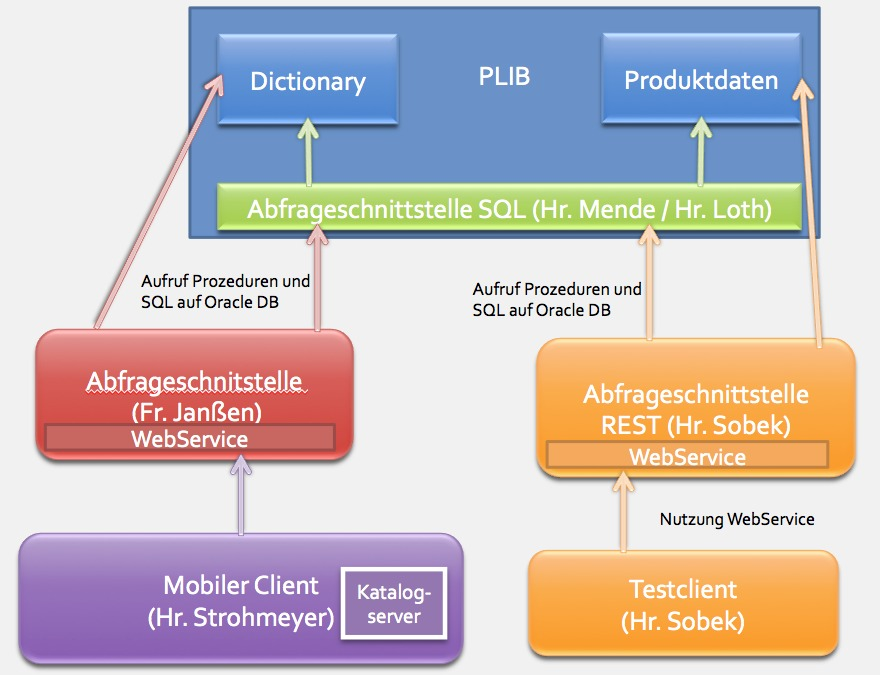
\includegraphics[width=0.75\textwidth]{images/gesamtkontext_plib.jpg}
	\caption{Gesamtkontext PLIB Abschlussarbeiten}
	\label{fig:gesamtkontext_plib}
\end{figure}

Die \autoref{tab.gesamtkontext} erläutert die \autoref{fig:gesamtkontext_plib} und listet dazu die jeweiligen Arbeiten und die zur Problemlösung betrachteten ISO-Standards auf.

% \cellcolor{<Farbe>}, \rowcolor{<Farbe>}, {\columncolor{<Farbe>}}, ändern die Hintergrundfarbe. 
\begin{table}[!hbt]\vspace{1ex}\centering
\scriptsize
\begin{tabular}{p{3cm}p{2.2cm}p{5cm}p{2.6cm}}
\toprule \rowcolor{mylightergray}
\textbf{Bezeichnung} & \textbf{Arbeit von} & \textbf{Erläuterung} &  \textbf{ISO Standards}\\
\midrule
Abfrageschnittstelle als \gls{Webservice} mit \gls{SOAP} &  Frau Janßen & Implementierung eines \glspl{Webservice} zur Auflösung von Konzept-Identifikatoren in Konzept-Dictionaries/Ontologien & ISO 29002-20 \\
\hline
PLIB, Dictionary und Produktdatenbank &  Herr Mende und Herr Loth & Meta- und Produktdatenbank sowie eine Abfrageschnittstelle basierend auf Oracle. Entwicklung von Abfrageschnittstellen mit Oracle Prozeduren & ISO 13584-42 \citep[Vergl.][]{iso13584-42}  \\
\hline
Mobiler Abfrageclient & Herr Lohmeyer & Entwicklung eines mobilen Abfrageclients basierend auf Android. Der Client nutzt die \glspl{Webservice} von Frau Janßen und beinhaltet einen eigenen Katalog\-server. & ISO 29002-10, ISO 13584-42 \\
\hline
Abfrageschnittstelle als \gls{Webservice} mit \gls{REST} für charakteristische Produktdaten & Herr Sobek & Entwicklung einer Schnittstelle zur Abfrage von charakteristischen Produktdaten. Die Schnittstelle wird als \gls{REST}ful \gls{Webservice} implementiert. & ISO 29002-31, ISO 29002-10 \\
\bottomrule
\end{tabular}
\caption{\label{tab.gesamtkontext}Erläuterung der Gesamtkontextabbildung}
\vspace{2ex}\end{table}

\subsection{Abgrenzung} \index{Identification Guide} \index{Abgrenzung} \index{Use Cases}\index{ISO 29002-10}

Die Arbeit umfasst die Implementierung der Use Cases nach \autoref{kap:Use_Cases}. Dies beinhaltet im wesentlichen den Teil 31 der ISO 29002 - einen Abfragestandard für charakteristische Produktdaten. 
Weiterhin wird für die Datenübertragung eine Implementierung des Teils 10 der ISO 29002 benötigt, siehe \autoref{fig:lieferketten}. 
Die Arbeit beinhaltet nicht die Implementierung eines \glspl{IG} nach ISO 22745-30. Dieser wird in der Praxis von einem Klienten für eine sinnvolle Vorauswahl der für sich oder seine Organisation benötigten Attribute der Teile verwendet. Jeder Klient definiert für seinen Kontext sinnvolle Attribute und Teiledaten und definiert diese mit Hilfe des Schemas der ISO 22745-30. Dies kann mittels eines Webformulars auf Klientenseite erfolgen oder als allgemeines Formular mit z.B. \gls{Excel}, welches die für den/die Klienten relevanten Attribute der Produkte, die abgefragt werden sollen, enthält. Für mehr Informationen zum \gls{IG} siehe \autoref{kap:identification_guide}.

%Beispiel: bild mit footnote
\begin{figure}[htbp]
	\centering
		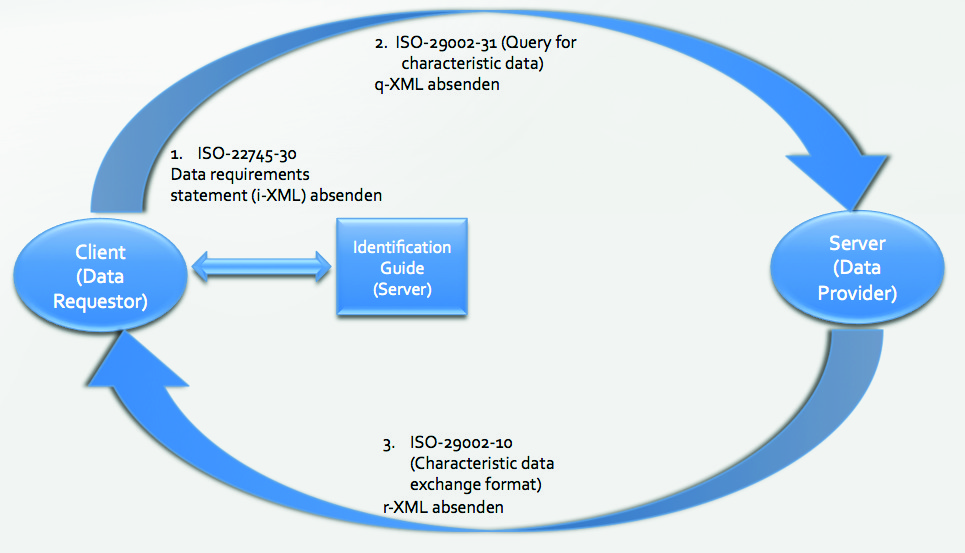
\includegraphics[width=0.90\textwidth]{images/lieferketten_plib.jpg}
		\caption[Lieferketten]{Lieferketten\footnotemark}
	\label{fig:lieferketten}
\end{figure}
\footnotetext{Abbildung entnommen und abgewandelt aus Benson, Converting Standard Terminology into usable Metadata, 2008 - später in ähnlicher Form auch in Uiterwyk, Die Bedeutung der Merkmalleisten bei eCl@ss, 2012 zu finden.}

\subsection{Vorgaben}\index{Vorgaben}\index{Oracle}

Für die Implementierung sind folgende nichtfunktionale Anforderungen vorgegeben:
\begin{description}
\item[Datenbanksystem Oracle] Dieses beinhaltet die PLIB Datenbank samt Abfrageprozeduren und stellt als Teiledatenbank die Basis dar. Dies wird vom Fachbereich bzw. von den Studenten Herr Mende/Herr Loth gestellt.
\item[Webservice] Auf Grund der hohen Verbreitung und Integrationsmöglichkeiten soll die Schnittstelle als \gls{Webservice} entwickelt werden. Die ISO 29002-31 schlägt als Beispiel eine E-Mail-Schnittstelle vor. Siehe \autoref{fig:datenfluesse}, welche besagt:
\begin{quotation}
Transport: not specified in ISO/TS 29002 (could use email) Payload XML.Query XML schema in ISO/TS 29002-31
\end{quotation}
Dies ist folglich nur ein Vorschlag. 
\item[PLIB Datenbankprozeduren] Die vorhandenen Prozeduren zum Zugriff auf die PLIB Datenbank sollen so weit wie möglich verwendet werden. 
\end{description}

\subsection{Datenflüsse} \index{Datenflüsse} \index{Webservice}\index{ISO 29002-10}\index{ISO 29002-31}
Das System soll einen \gls{Webservice} zur Verfügung stellen. Dieser \gls{Webservice} soll eine XML Datei gemäß ISO 29002-31 entgegennehmen. Die entsprechende Verarbeitung des XMLs, sowie die logische Transformation der Anfrage zur Abfrageschnittstelle der Datenbank wird vom System vorgenommen. Die Antwort der Datenbank soll wieder zurücktransformiert werden und als Katalog-XML Datei gemäß ISO 29002-10 zurückgeliefert werden.
 
Der gerahmte Bereich im unteren Teil der \autoref{fig:datenfluesse} zeigt in der Datenflussabbildung, was implementiert werden soll. Das Zielsystem, gleichsam das System, welches die Anfrage erhält, wird hier als \enquote{Catalogue Server} bezeichnet. 
Die Kommunikation des Klienten mit dem Location Server, Terminology Server und dem Ontology Server ist Teil der Abschlussarbeit von Fr. Janßen \citep[Vergl.][]{janssen}. 
Die Abfrageprozeduren des Katalogservers auf Datenbankebene ist Aufgabe von Herrn Mende. Zur Zeit der Abgabe dieser Arbeit, war die Arbeit von Herrn Mende noch in Bearbeitung\footnote{Die Basis dieser Abschlussarbeit ist ein stabiler Implementierungsstand, welcher von Herrn Mende geliefert wurde.}. 

\begin{figure}[htbp]
	\centering
		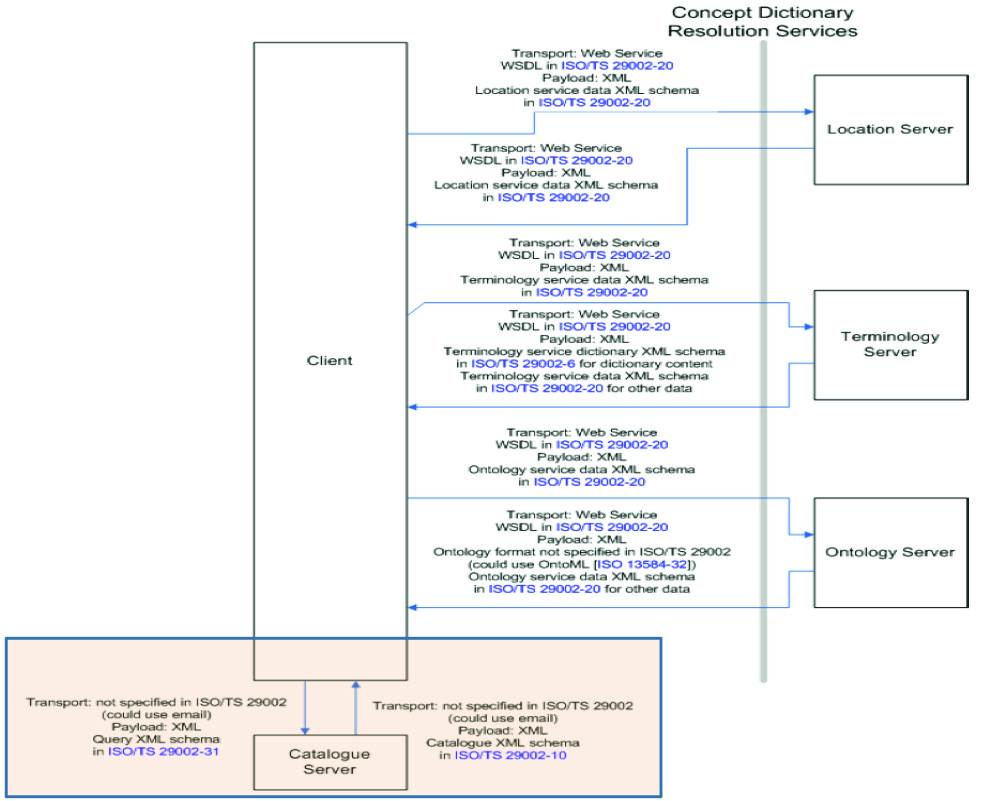
\includegraphics[width=0.90\textwidth]{images/datenfluesse_plib.jpg}
	\caption[Datenflüsse]{Datenflüsse\footnotemark}
	\label{fig:datenfluesse}
\end{figure}
\footnotetext{Quelle: entnommen ISO 29002-31 Figure 3 - Major Dataflows. Zur besseren Visualisierung wurde der untere Bereich farblich hervorgehoben.}

\setchapterpreamble[u]{%
\dictum[René Descartes]{Vor eine Frage gestellt, die wir vollständig verstanden haben, müssen wir sie von jeder überflüssigen Darstellung abstrahieren, sie auf ihre einfachste Form reduzieren und sie in möglichst kleine Teile zerlegen, die wir dann aufzählen. \dots}}
\chapter{Analyse und Definition der Anforderungen } \index{Analyse und Definition der Anforderungen}\label{kap:analyse_und_definition}

Das \autoref{kap:aufgabenbeschreibung} erwähnt mehrere ISO Standards, welche zur Lösung der Problemstellung unterstützen können. In diesem Kapitel wird der ausgewählte ISO Standard ISO 29002-31 sowie der Standard ISO 22745-30 analysiert, um festzustellen, welche Anforderungen mit Hilfe dieser Standards umgesetzt werden können. 

Mittels den Erkenntnissen der Analyse werden Use Cases erarbeitet. 

\section{Analyse der ISO 29002-31 - Exchange of characteristic data}\label{kap:analyseiso2900231}\index{ISO 29002-31}

Ziel der Analyse ist es, herauszufinden, ob die ISO-Norm zur Erfüllung der Anforderungen ausreichend ist, wie mit der ISO-Norm die Anforderungen umgesetzt werden können und ob gegebenenfalls weitere ISO-Normen zur Erfüllung der Anforderungen betrachtet werden müssen. 

Die gesamte Analyse der ISO 29002-31 mit Beschreibung der einzelnen Datencontainer findet sich in \autoref{kap:analyse2900231}. Die Analyse zeigt anhand von Beispielen auf, welche Abfragen mit der ISO 29002-31 möglich sind.

Zusammenfassend aus der Analyse ergeben sich folgende Abfragemöglichkeiten:
\begin{description}
\item[Simple Query] Eine Abfrage nach eindeutigem Identifier eines Konzeptes, mit der Möglichkeit der Einschränkung nach Eigenschaften eines Konzeptes (Projektion). Ferner ermöglicht der Simple Query die Übergabe bekannter Daten eines konkreten Teiles, nach denen gesucht und ein entsprechend passendes Ergebnis geliefert wird. Siehe dazu \autoref{sec:query}.
\item[Parametric Query] Ermöglicht die Abfrage nach eindeutigem Identifier eines Konzeptes und zusätzlich die Einschränkung einer Eigenschaft nach konkretem Wert (Selektion). Dies erfolgt mittels Angabe einer characteristic\_data\_query\_expression. Siehe dazu \autoref{sec:characteristicdataqueryexpression}.
\end{description}

Die konkreten Query Beispiele finden sich dazu in \autoref{kap:query_beispiele}.

\section{Analyse ISO 22745-30 - Identification Guide}\label{kap:identification_guide}\index{ISO 22745-30}

Ein \gls{IG} beschreibt, welche Daten für ein Objekt benötigt werden, damit diese überhaupt sinnvoll für einen bestimmten Zweck eingesetzt werden können. Der Käufer, Produktmanager oder Benutzer definiert die Anforderungen an die Daten. Ein  \enquote{Datenanforderungsstatement} wird als ein i-xml, eine \gls{IG}-xml Datei, erzeugt. Siehe dazu \autoref{fig:lieferketten}. 

Es wird die Frage beantwortet, welche Daten und Eigenschaften zu einem bestimmten Konzept eines Objektes benötigt werden, um den Artikel beispielsweise zu kaufen oder sinnvoll zu verwalten. Diese Anforderungen werden von der Abfrageseite (Kundenseite) definiert, also diejenige, die Daten abfragen möchte \citep[Vergl.][]{bensonQuality}. 

Ein Identification Guide referenziert Konzepte eines Dictionaries um Datenanforderungen einer bestimmten Klasse zu beschreiben \citep[Vergl.][Kap. 5]{iso22745-30}.

Ein Datenempfänger kann eine Organisation oder eine Gruppe von Organisationen oder Firmen sein, welche ähnliche Datenanforderungen haben. Somit wird eine Identification Guide Gruppe von einer speziellen Organisation verwaltet, welche wiederum selbst Datenempfänger sein kann.  

Es kann somit festgehalten werden, dass für die Erfüllung der Aufgabenbeschreibung nach \autoref{kap:aufgabenbeschreibung} eine Implementierung des Standards ISO 22745-30 nicht notwendig ist, da dieser Standard eine zusätzliche Einschränkung der Konzepte und benötigten Daten auf Anfrageseite beschreibt. 
Die Abfrage gemäß einer SQL-Selektion und -Projektion ist mit dem Standard 29002-31 möglich. 

Basierend auf dieser Erkenntnis zeigt \autoref{fig:query_kombinationen} mögliche Abfrageinhalte und bewertet, ob diese umgesetzt werden müssen. Hierbei werden die Attribute \enquote{item\_description} und \enquote{data\_specification} nicht betrachtet.

\begin{figure}[htbp]
	\centering
		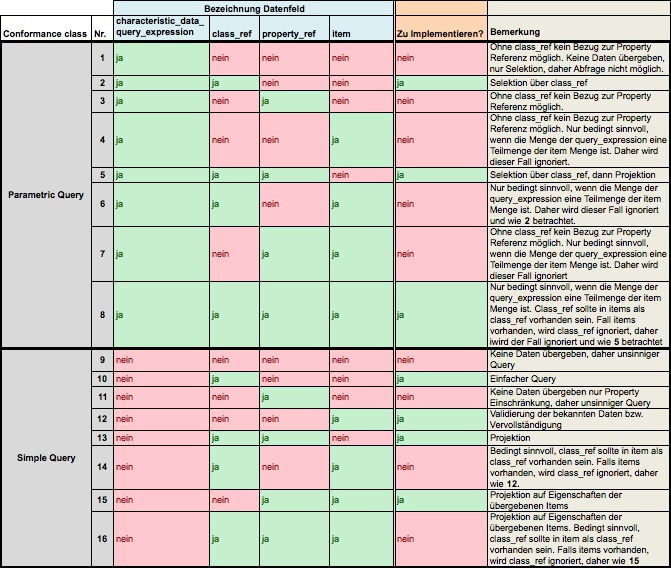
\includegraphics[width=0.90\textwidth]{images/queries.jpg}
	\caption{Mögliche Abfragen anhand der Kombination der Daten in XML Query}
	\label{fig:query_kombinationen}
\end{figure}

\section{Anwendungsfälle}\label{kap:Use_Cases}

Dieser Abschnitt beschreibt mögliche Anwendungsfälle\footnote{Use Case. Im weiteren Verlauf wird, gerade auch in den Anwendungsfallbeschreibungen von Use Cases gesprochen. Im deutschen Sprachraum ist das englische allgemein bekannte Äquivalent \enquote{Use Case} für Anwendungsfall eher geläufig als das deutsche, daher wird darauf verzichtet an manchen Stellen die Begrifflichkeiten einzudeutschen.} die sich aus ISO 29002-31 ergeben. 
Es wird beispielhaft ein Use Case aufgelistet und erläutert. Alle weiteren Use Cases sind in \autoref{kap:analyse_use_cases} zu finden. 

Die Query-Code-Beispiele sind gekürzt, d.h. es werden die referenzierten Schemata-Namen gemäß XSD nicht aufgeführt. 

\subsection{Was ist ein Use Case?}

Alistair Cockburn schreibt dazu \citep[Vergl.][Kap. 1.1]{cockburn2000}:

\begin{quotation}
\enquote{A use case captures a contract between the stakeholders of a system about its behavior. The use case describes the system’s behavior under various conditions as it responds to a request from one of the stakeholders, called the primary actor. The primary actor initiates an interaction with the system to accomplish some goal. The system responds, protecting the interests of all the stake- holders. Different sequences of behavior, or scenarios, can unfold, depending on the particular requests made and conditions surrounding the requests. The use case collects together those different scenarios.}
\end{quotation}

\gls{Stakeholder}\footnote{Stakeholder sind Projektbeteiligte, gleichsam Personen oder Institutionen und Dokumente, die in irgendeiner Weise vom Betrieb des Systems betroffen sind.} erwarten folglich ein gewisses Verhalten des Systems unter bestimmten Bedingungen. Dieses Verhalten des Systems in Interaktion mit Akteuren wird durch \glspl{Use Case} beschrieben.

\bild{usecases_plib.jpg}{10cm}{Use Case Übersicht}{Use Case Übersicht}

\subsection{Akteure}
Bei der Implementierung geht es um die Erstellung einer Software-Schnittstelle als \gls{Webservice}. Das bedeutet, dass diese Schnittstelle ohne eine Benutzeroberfläche nicht sinnvoll für einen menschlichen Akteur nutzbar ist. In den nachfolgenden Anwendungsfällen wird vom Akteur \enquote{Klient} gesprochen. Der Klient ist allgemein ein Nutzer der Schnittstelle, sei es als menschlicher Akteur welcher über eine Bedienerinterface die Schnittstelle benutzt oder eine direkte Maschinennutzung. Ein Beispiel für eine Maschinennutzung kann eine Anwendung sein, welche automatisiert die Schnittstelle aufruft und Daten abfragt.    

\subsection{Use Case Beschreibungen}

Da \glspl{Use Case} auf verschiedene Weise verfasst werden können, werden hier als Vorlage die \gls{Use Case} Beschreibungen aus dem Kurs Software Engineering I übernommen, da diese Vorlage sehr übersichtlich, knapp und präzise ist \citep[Vgl.][S. 120ff]{sixse1}. 

\subsubsection{Alle charakteristischen Daten eines Produkts abfragen}

{\small

\begin{description}
     \item[use case] Charakteristische Daten abfragen
     \item[  actors]~\\
     Klient
     \item[  precondition]~\\
     Der Klient verwendet einen gültigen Identifier.
     \item[  main flow]~\\
     Der Klient gibt einen Identifier (\gls{IRDI}) eines Konzeptes von Elementen ein und sendet eine Anfrage ab. Die Anfrage wird auf Gültigkeit überprüft. Als Antwort bekommt er ein oder mehrere Datensätze von \glslink{item}{Teilen} mit den entsprechenden charakteristischen Daten \footnote{property\_values, ISO 29002-10 Kapitel 5.2.4} des \glslink{item}{Teils} mit dem übergebenen Identifier zurück.
     \item[  postcondition]~\\
     Alle Daten aller \glslink{item}{Teile} der gewählten Konzepte des Identifiers wurden zurückgegeben.    
     \item[  alternative flow] Properties auswählen ~\\
     Zusammen mit dem Identifier übergibt der Klient einen oder mehrere Property-Identifier und sendet diese erweiterte Anfrage ab.    
     \item[  postcondition]~\\
     Die mittels Property-Identifier ausgewählten Daten aller  \glslink{item}{Teile} der gewählten Konzepte wurden zurückgegeben.    
     \item[  alternative flow] Keine Eigenschaftswerte vorhanden ~\\
     Für das mittels Identifier angefragte \glslink{item}{Teil} sind keine Eigenschaftswerte vorhanden.    
     \item[  postcondition]~\\
     Es werden keine Daten zurückgeliefert.   
     \item[  exceptional flow] Ungültige Identifier oder ungültige Anfrage ~\\
     Der oder die übergebenen Identifier oder die gesamte Anfrage ist gemäß Spezifikation ungültig.  
     \item[  postcondition]~\\
     Es wird eine Fehlermeldung zurückgegeben.  
     \item[end] Charakteristische Daten abfragen
\end{description}

~\\

} %end small

\subsubsection{Beispiel}\label{lab:schraubendreher}

Ein Schraubendreher könnte folgendermaßen in einer Produktdatenbank repräsentiert werden:

\begin{description}
\item[Klassen-Identifier] 0173-1\#01-AAA352\#4 
\item[Länge] 300mm
\item[Typ] Kreuz
\item[Spannungsfest] ja
\end{description}

Korrekterweise müsste anstatt der Attribute wie Länge oder Typ ebenfalls ein Identifier stehen. Die Bezeichnungen sind hier zur besseren Lesbarkeit aufgelöst. 

Um alle Eigenschaften (Properties) wie \enquote{Länge}, \enquote{Typ} und \enquote{spannungsfest} zu erhalten, muss folgende Abfrage gesendet werden: 
\begin{quotation}
\enquote{Gib mir alle \glslink{item}{Teile} und alle Properties der Klasse mit dem Identifier 0173-1\#01-AAA352\#4 (Schraubendreher).}
\end{quotation}

Das Ergebnis ist ein \gls{item} mit allen Attributen (Properties) der gewünschten Konzepte und gegebenenfalls vorhandenen Unterkonzepte. In diesem Falle genau sind es die oben angegebenen Werte.

Die XML-Abfrage sieht wie folgt aus:

\begin{lstlisting}[caption=Query Beispiel - alle Daten abfragen, language=XML, label=UseCaseDatenabfragen]
<?xml version="1.0" encoding="UTF-8"?>
<qy:query xsi:schemaLocation="...query query.xsd" xmlns:xsi="http://www.w3.org/2001/XMLSchema-instance" xmlns:cat="...catalogue" xmlns:val="...value" xmlns:qy="...query" xmlns:bas="...basic">
	<qy:class_ref>0173-1#01-AAA352#4</qy:class_ref>
</qy:query>
\end{lstlisting}

Eine Abfrage, welche als Projektion die Properties der Klasse auswählt, die zurückgeliefert werden sollen, könnte lauten: 
\begin{quotation}
\enquote{Gib mir alle \glslink{item}{Teile} und die Properties Länge und Typ der Klasse mit dem Identifier 0173-1\#01-AAA352\#4 (Schraubendreher).}
\end{quotation}

Das Ergebnis ist ein \gls{item} mit den gewünschten Attributen (Properties). 

Die XML-Abfrage lautet:
\begin{lstlisting}[caption=Query Beispiel - Daten abfragen mit Propertyeinschränkung (Projektion), language=XML, label=lst:UseCaseDatenabfragenProperty]

<?xml version="1.0" encoding="UTF-8"?>
<qy:query xsi:schemaLocation="...query query.xsd" xmlns:xsi="http://www.w3.org/2001/XMLSchema-instance" xmlns:cat="...catalogue" xmlns:val="...value" xmlns:qy="...query" xmlns:bas="...basic">
	<qy:class_ref>0173-1#01-AAA352#4</qy:class_ref>
	
	<!-- identifier von typ und laenge werden uebergeben -->
	<qy:property_ref>0173-1#01-BBB111#1 0173-1#01-BBB222#1</qy:property_ref> 
	
</qy:query>
\end{lstlisting}

\autoref{lst:UseCaseDatenabfragenProperty} beinhaltet ein XML-Attribut property\_ref. Das wird mit einem oder mehreren gewünschten Property Identifiern gefüllt. Werden mehrere Identifier angegeben, so sind diese mit Leerzeichen zu trennen. In diesem Beispiel sind zwei angegeben, das bedeutet, dass diese beiden Eigenschaftswerte abgefragt werden.


\section{Zusammenfassung des Kapitels}

Das Ergebnis der Analyse der Standards ISO 29002-31 und 22745-30 ergibt, dass diese Beschreibungen für die Lösung der Problemstellung, die Entwicklung einer \gls{Abfrageschnittstelle} analog zur SQL-Selektion und Projektion der Standard ISO 29002-31, ausreichend sind. Sowohl Projektion als auch Selektion ist dadurch möglich. ISO 22745-30 beschreibt als \gls{IG} eine weitere klientseitige Einschränkung der abzufragenden Daten. Man stelle sich eine Einschränkung (Definition einer Teilmenge) durch ein Formular vor. Das Formular schränkt die abzufragenden Daten auf die tatsächlich benötigte Menge von Daten gegebenenfalls stark ein und gibt ebenfalls den Typ der Daten vor. Dies wird durch Referenzieren auf Konzepte eines Dictionaries erreicht.

Aus den Anforderungen wurden sinnvolle \glspl{Use Case} formuliert, welche das Verhalten des Systems beschreiben sollen.  

\setchapterpreamble[u]{%
\dictum[Douglas Adams]{A common mistake that people make when trying to design something completely foolproof is to underestimate the ingenuity of complete fools. \dots}}
\chapter{System- und Softwareentwurf} \index{System- und Softwareentwurf}\label{kap:systemundsoftwarentwurf}


Dieses Kapitel beschreibt den System- und Softwareentwurf sowie die Auswahl der Umgebung, Plattform, Software, Programmiersprache und Frameworks.

\section{Auswahlprozess}

Teil der Aufgabe der Arbeit ist es, für das System im Rahmen der nichtfunktionalen Anforderungen eine geeignete Laufzeitumgebung zu schaffen. Dafür sind einige Entscheidungen zu treffen. 

\subsection{Webservice}\index{Webservice}\label{sec:webservice}
Wenn von \glspl{Webservice} gesprochen wird, dann werden meistens \gls{SOAP}-basierte \glspl{Webservice} gemeint. Allerdings gibt es die sogenannten \gls{SOAP}-basierten \glspl{Webservice} als auch die \gls{REST}ful \glspl{Webservice}. Anforderung ist es ein \gls{Webservice} zu implementieren. Dazu muss entschieden werden, ob ein \gls{SOAP}-basierter oder \gls{REST}ful \glspl{Webservice} implementiert werden soll. \index{REST!RESTful}

\subsubsection{Definition}

\begin{quotation}
\enquote{\glslink{Webservice}{Web services} provide the means to integrate disparate systems and expose reusable business functions over \gls{HTTP}. They either leverage \gls{HTTP} as a simple transport over which data is carried (e.g., \gls{SOAP}/\gls{WSDL} services) or use it as a complete application protocol that defines the semantics for service behavior (e.g. RESTful services) \citep[S. 2][]{robinsonService}}	
\end{quotation}

\subsubsection{SOAP/WSDL Webservice}\index{SOAP}\index{WSDL}\index{Webservice}
Frau Janssen hat in ihrer Abschlussarbeit einen \glspl{Webservice} nach ISO 29002-20 mittels einem  \gls{SOAP}/\gls{WSDL} \glspl{Webservice} implementiert \citep[vgl.][]{janssen}. Die ISO 29002-20 verweist in Annex-B auf entsprechende \gls{WSDL}-Definitionen. 
Ich möchte an dieser Stelle darauf verzichten, die Einzelheiten eines SOAP/WSDL Webservice zu erläutern und verweise auf Frau Janßens Abschlussarbeit \citep[vgl.][Kap. 3]{janssen}. 

Es sei an dieser Stelle kurz erwähnt, dass \glspl{Webservice} auf \gls{SOAP}/\gls{WSDL} basierend ein W3C\footnote{World Wide Web Consortium - http://www.w3.org} Standard sind. Dies ist häufig auch ein Kriterium, weshalb in der Industrie \gls{SOAP}/\gls{WSDL} \glspl{Webservice} stark verbreitet sind. 

\subsubsection{RESTful Webservice}\index{RESTful Webservice}\index{REST@\textbf{REST}} \index{REST!RESTful} \index{REST!RESTful Webservice}
\gls{REST}ful Webservices sind per se kein Standard sondern eher ein Programmierparadigma respektive ein Architekturmuster. 
Stefan Tilkov schreibt dazu in seinem Buch \enquote{Rest und HTTP: Einsatz der Architektur des Web für Integrationsszenarien} \citep[S.10][]{tilkovrest}, folgendes:

\begin{quotation}
\enquote{...Im Rahmen seiner Dissertation - beendet im Jahre 2000 - abstrahierte Fielding\footnote{Anmerkung des Autors: Roy Thomas Fielding} von der konkreten Architektur, die \gls{HTTP} zugrunde liegt, und legte den Schwerpunkt auf die Konzepte anstatt auf die konkrete Syntax, die Details des Protokolldesigns und die vielen Kompromisse, die aus Kompatibilitätsgründen eingegangen werden mussten. Als Ergebnis entstand der Architekturstil \gls{REST}. Dieser ist somit eine Stufe abstrakter als die \gls{HTTP}-Architektur: Theoretisch könnte man die Prinzipien von \gls{REST} auch mit einem neu erfundenen Satz von Protokollen umsetzen. In der Praxis ist jedoch tatsächlich nur das Web als konkrete Ausprägung des Architekturstils relevant...}
\end{quotation}
\citep[Vgl. auch][]{fieldingrest}

\subsubsection{Fazit}
Die Analyse aus \autoref{kap:analyse_und_definition} zeigt, dass eine Abfrage (Query) gemäß Standard als XML dargestellt wird. Diese XML-Dateien müssen folglich an das System gesendet werden. Demnach ist eine Lösung mittels \gls{SOAP} \gls{Webservice} als auch \gls{REST}ful \gls{Webservice} denkbar. 
Es wurde ein \gls{REST}ful \gls{Webservice} ausgewählt. Die Gründe stellen sich wie folgt dar:

\begin{description}
\item[Einfache Implementierung] Da \gls{REST}ful Webservices auf dem \gls{HTTP} Protokoll basieren und ferner sehr gute und geeignete Frameworks für Java vorhanden sind, siehe \autoref{sec:bibliotheken_und_frameworks}, stellt sich für Web Entwickler die Implementierung als einfach heraus. \gls{SOAP} \glspl{Webservice} sind per se etwas komplexer, da \gls{SOAP} ein eigenes Protokoll darstellt. 
\item[Payload XML] Der Payload des Anfrage-Queries wird als XML angegeben (siehe \autoref{fig:datenfluesse}. Als mögliche Übertragung wird email angegeben. Für die Anforderungen dieser Arbeit bedeutet dies eine Implementierung eines \glspl{Webservice}, welcher die XML-Repräsentation des Queries als Payload mittels XML überträgt. Folglich könnte sowohl \gls{SOAP} als auch \gls{REST} benutzt werden. Voraussetzung ist eine definierten Schnittstelle, welche lediglich ein XML als Payload akzeptiert. 
\item[Kein Vorteil bei SOAP] Somit hat \gls{SOAP} keinen Vorteil gegenüber \gls{REST}. Der Vorteil würde darin bestehen, wenn \gls{SOAP} selbst die Operationen anbietet (definiert in der \gls{WSDL}). Das hat den Nachteil, dass die wohlgeformte vorgegebenen Schemata query.xsd, in der Form nicht genutzt werden können. Es muss somit eine Einbindung in \gls{SOAP} erfolgen.
 \item[Vorteil des Payloads] Der klare Vorteil bei der Variante eine Query XML-Datei gemäß query.xsd Schema des Standards als Payload zu versenden ist der, dass eine Validierungsprüfung der XML gegen vorhandene definierte Regeln des Schemas erfolgen kann (z.B. gültige \gls{IRDI}), ferner können aus dem Schema passende Modellklassen zur Verarbeitung und Speicherung der Query-Daten in der Applikation generiert werden. Mehr Informationen gibt es in \autoref{sec:modellgenerierung}. 
\item[SOAP Webservice bereits im Einsatz] Ein weiterer Grund ist der, dass Frau Janßen in Ihrer Abschlussarbeit bereits einen SOAP-Webservice einsetzt. Nennen wir es Vielfältigkeit der Technologien im Fachbereich, jedenfalls bietet es die Möglichkeit eine weitere Technologie zu betrachten, einzusetzen und ggfs. zu vergleichen. 
\end{description}

\subsection{Plattform} \index{Apache Tomcat} \label{sec:plattform}\index{Web Server}\index{Web Container}
Als Laufzeitumgebung kann prinzipiell ein beliebieger Web Container bzw. Web Server ausgewählt werden, welcher Webservices, sei es \gls{REST}ful \glspl{Webservice} oder \gls{SOAP} \glspl{Webservice}, unterstützt. 
Es wurde der \gls{Apache Tomcat} Server in der Version 7 ausgewählt. Das ist ein üblicher Web Container (Web Server), welcher mit entsprechenden Frameworks bzw. Bibliotheken sowohl \gls{SOAP} als auch \gls{REST}ful \glspl{Webservice} anbieten kann. 

Folgende Server sind zum Einsatz ebenfalls möglich:

\begin{description}
\item[Jetty] http://www.eclipse.org/jetty/
\item[Tomcat] https://tomcat.apache.org/
\item[JBoss] https://www.jboss.org/overview/
\end{description}

Festzuhalten sei noch, dass es sich beim JBoss Server um einen sogenannten Application Server handelt. Er verfügt zusätzlich zur Web Container Funktionalität noch über weitere Dienste, wie beispielsweise Transaktionsmanagement, Securitymanagement oder verteilte Applikationsunterstützung. 

\subsection{Bibilotheken und Frameworks} \index{Bibilotheken und Frameworks}\label{sec:bibliotheken_und_frameworks}
\begin{description}

\item[Jersey] Framework zur Erstellung von RESTful Web Services \index{Jersey}\gls{Jersey}
\item[JSF2.0] Komponentenbasiertes Web Framework zur Erstellung von Benutzeroberflächen \index{JSF2.0}
\item[Spring] Dependency Injection Framework. Bietet darüber hinaus noch weitere Komponenten an. Ausgewählt wurde unter anderem \gls{Spring} JDBC und \gls{Spring} Data Oracle, welche einfacheren Zugriff auf relationale Datenbanken sowie auf Prozeduren von relationalen Datenbanken ermöglicht. \index{Spring} \index{Spring!Data Oracle}
    
\end{description}

\todotext{Eine detaillierte Erklärung der Frameworks nötig, Erläuterung des Nutzens und weshalb diese ausgesucht wurden. Ggfs in Anhang}

\subsection{Programmiersprache}\index{Programmiersprache}
Vorgegeben ist die Umsetzung eines \glspl{Webservice}. Diese lassen sich in fast allen aktuellen Programmiersprachen entwickeln, folglich kann prinzipiell jede Sprache ausgewählt werden die Webservices anbieten kann.  

Es wurde die Sprache Java gewählt, da diese zum einen in der aktuellen Industrie stark verbreitet und zum anderen der Autor dieser Arbeit seit vielen Jahren damit vertraut ist. Ferner besteht hier eine Abhängigkeit zur Auswahl der Plattform gleichsam des Web Containers, siehe \autoref{sec:plattform}. Beim Einsatz von Java ist man an einen Web Container (Web Server) gebunden, welcher auch Java unterstützt. 

Ein weiterer Aspekt ist, dass Software welche mit Java entwickelt wurde im Prinzip auf jedem Betriebssystem lauffähig, und somit portierbar ist. Dies ist zwar keine Anforderung des Projektes, aber ermöglicht die Arbeit und Entwicklung in beliebigen Systemen. 

\section{Softwaredesign und Architektur}\index{Softwarearchitektur}\index{Softwaredesign}

\subsection{Bausteinsicht}\index{Software-Bausteine}
\begin{quotation}
Die Bausteinsicht bildet die Aufgaben des Systems auf Software-Bausteine oder -Komponenten ab.
 \citep[S. 98ff][]{starke}	
\end{quotation}

Es soll mit Hilfe dieser Sichten ein Überblick über den Aufbau des Systems und den Abhängigkeiten der einzelnen Komponenten geschaffen werden. Dazu wird das System im top-down Ansatz aufgezeigt und verfeinert. 

\subsection{Kontextabgrenzung - Systemüberblick und angrenzende Systeme}\index{Kontextabgrenzung}

Die Kontextabgrenzung zeigt das System im Zusammenspiel mit anderen Systeme und zeigt somit gleichsam die Systemgrenzen auf. 

\begin{figure}[!htbp]
	\centering
		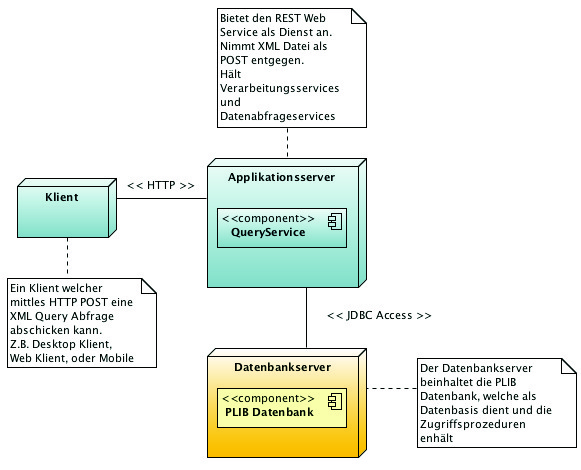
\includegraphics[width=0.7\textwidth]{images/bausteinsicht_plib_level0.jpg}
	\caption{Bausteinsicht - Kontextabgrenzung}
	\label{fig:bausteinsicht_level0}
\end{figure}

\begin{description}
\item[Klient] Der Klient stellt den Nutzer des Query Services dar. Er erzeugt das XML File, welches als Query an den Service geschickt wird. Der Transport erfolgt über das HTTP Protokoll. \index{Klient}
\item[Applikationsserver] Der Applikationsserver ist der Hauptbaustein. Dieser Baustein enthält alle entwickelten Komponenten. Sichtbar von außen ist der QueryService, dieser Service ist ein REST WebService und nimmt XML-Dateien als Payload eines POST Requests entgegen. \index{Applikationsserver}
\item[Datenbankserver] Der Datenbankserver beinhaltet die PLIB Datenbank mit den entsprechenden Zugriffsprozeduren auf die Daten. \index{Datenbankserver}\index{PLIB}
\end{description}

\subsection{Level 1 - Plib characteristic query} \index{Characteristic query}

Die Bausteinsicht Level 1 zeigt alle Komponenten des entwickelten Systems auf und deutet die externen Schnittstellen an. Mittels <<use>> Beziehungen erkennt man die Abhängigkeiten der einzelnen Komponenten. 

\begin{figure}[htbp]
	\centering
		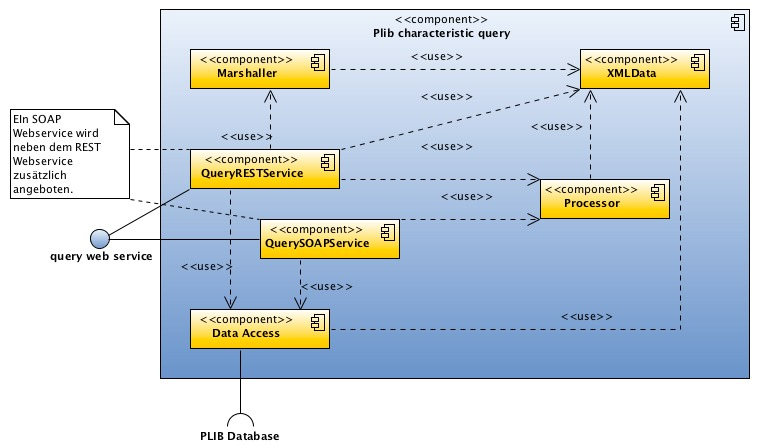
\includegraphics[width=0.98\textwidth]{images/bausteinsicht_plib_level1.jpg}
	\caption{Bausteinsicht - Level 1}
	\label{fig:bausteinsicht_level1}
\end{figure}

\begin{description}
\item[QueryService] Der Zweck dieser Komponente ist das Entgegennehmen des Requests (Query-XML File), das Weiterleiten an die weiterverarbeitenden Komponenten und letztlich das Zurücksenden der Rückantwort (Katalog-XML). Bietet nach Außen die \gls{Webservice}-Schnittstelle an.
\item[Data Access] Diese technische Komponente beinhaltet die Zugriffsschicht auf die externe Datenbankschnittstelle und bietet entsprechend vereinfachte Abfrageschnittstellen für die anderen Komponenten an. 
\item[Marshaller] Eine weitere technische Komponente, diese ist für das Einlesen und Validieren der eingegangenen Query-XML Datei verantwortlich. Ferner transformiert diese Komponente die Informationen aus der Query-XML nach Validierung in das im System benutze Datenmodell aus der Komponente XMLData.
\item[XMLData] Beinhaltet das Datenmodell des Systems. Sowohl die eingehenden Query-XML Daten, als auch die ausgehenden Katalog-XML Daten werden intern in ein entsprechendes Model zur Verarbeitung abgelegt, so dass darauf gearbeitet werden kann.  
\item[Analyser] Diese Komponente ist für die Analyse des Queries, welches bereits als Modell vorliegt, verantwortlich. Erkennt ob es sich um einen \enquote{Simple Query} oder um einen \enquote{Parametric Query} handelt und leitet den Query zur Weiterverarbeitung an die Handler-Komponente weiter. 
\item[Handler] Erhält den Query vom Analyser und verarbeitet gemäß der Erkennung vom Analyser den Query weiter. Dazu werden die Querydaten gemäß des Datenbankmodells transformiert und die Data Access Komponente aufgerufen. Die Antwort der Data Access Komponente wird in das entsprechende Modell für die Katalogdaten umgewandelt und zurück an den Handler geleitet.  
\end{description}

\subsection{Level 2 - Whiteboxansicht - Komponente XMLData}\index{Whiteboxansicht}

Die Komponente XMLData beinhaltet alle Datenmodelle für die beiden Hauptkonzepte \enquote{Query for characteristic data} nach. 

\begin{figure}[htbp]
	\centering
		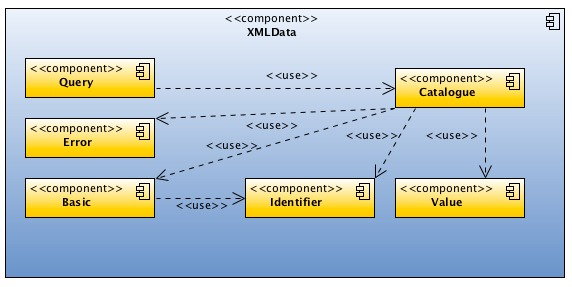
\includegraphics[width=0.82\textwidth]{images/bausteinsicht_plib_level2_xmldata.jpg}
	\caption{Bausteinsicht - Level 2 - Komponente XMLData}
	\label{fig:bausteinsicht_level2_xmldata}
\end{figure}

\begin{description}
\item[Query] Diese Komponente beinhaltet das Datenmodell des Queries nach ISO/TS 29002-31. 
\item[Catalogue] Diese Komponente beinhaltet das Datenmodell des Kataloges nach ISO/TS 29002-10. 
\item[Basic] Diese Komponente beinhaltet das Datenmodell von Basistypen nach ISO/TS 29002-4.
\item[Value] Diese Komponente beinhaltet das Datenmodell der Wertetypen nach ISO/TS 29002-10.
\item[Identifier] Diese Komponente beinhaltet das Datenmodell für Identifier (IRDI) nach ISO/TS 29002-5. 
\end{description}

\todotext{Whiteboxansicht der Komponente Handler und Analyser einfügen zum besseren Verständnisses, ggfs. alle detaillierten Whiteboxansichten in Anhang?!}

\setchapterpreamble[u]{%
\dictum[Johann Wolfgang von Goethe]{Es ist nicht genug, zu wissen, man muß auch anwenden; es ist nicht genug, zu wollen, man muß auch tun. \dots}}
\chapter{Implementierung} \index{Implementierung}\label{kap:implementierung}

\section{Configuration Management und Setup}\index{Configuration Managment}


\subsection{Maven}\index{Maven}
Maven ist ähnlich wie Ant ein Build und Deployment Werkzeug. Darüberhinaus ist es ein Dependency Management Werkzeug. Das bedeutet, dass Maven die abhängigen Artefakte und deren Versionen verwalten kann. 

\subsection{Apache Tomcat}\index{Apache Tomcat}
Als Web Container wird der \gls{Apache Tomcat} in der Version 7 eingesetzt. 

\subsection{Java 6}

\section{Web Service}\index{Web Service}\index{REST!RESTful Web Service}\label{kap:webservice}

Wie in Kapitel \todotext{XXX} erwähnt, wurde entschieden einen \gls{REST}ful Web Service zu erstellen. Dafür wurde das Jersey-Framework ausgewählt.

Folgende Schritte sind notwendig um einen \gls{REST}ful Webservice mit Jersey zu erstellen: 

\subsection{Servlet Konfiguration in web.xml} \index{Jersey}

In die Konfigurationsdatei web.xml des Webcontainers (hier \gls{Apache Tomcat}) muss das Servlet für \gls{Jersey} hinzugefügt werden, so dass \gls{Web Service} Anfragen an dieses Servlet möglich sind. 

\autoref{lst:jerseywebxmlconfig} zeigt den Ausschnitt aus der web.xml des \gls{PLIB}-Projektes. 

 \begin{lstlisting}[caption=Jersey Servlet Konfiguration in web.xml, language=XML, label=lst:jerseywebxmlconfig]
 <!-- configure jersey REST-Web Service Servlet -->
    <servlet>
        <servlet-name>jersey-servlet</servlet-name>
        <servlet-class>com.sun.jersey.spi.container.servlet.ServletContainer</servlet-class>
        <init-param>
            <param-name>com.sun.jersey.config.property.packages</param-name>
            <param-value>de.feu.plib.webservice.rest</param-value>
        </init-param>
        <load-on-startup>1</load-on-startup>
    </servlet>
 \end{lstlisting}   
 
Ferner muss in der web.xml ein sogenannter \enquote{Mappingeintrag} angelegt werden. Hierdurch wird dem Web Server mitgeteilt, bei zu welchem Servlet Anfragen an eine bestimmte URL zur Verarbeitung geleitet werden sollen. 
 
  \begin{lstlisting}[caption=Jersey Servlet Mappingkonfiguration in web.xml, language=XML, label=lst:jerseywebxmlconfigmapping]
    <servlet-mapping>
        <servlet-name>jersey-servlet</servlet-name>
        <url-pattern>/rest/*</url-pattern>
    </servlet-mapping>
 \end{lstlisting}  
 
Das Konfigurationbeispiel in \autoref{lst:jerseywebxmlconfigmapping}  besagt, dass das Servlet mit dem Namen \enquote{jersey-servlet}, welches im Beispiel \autoref{lst:jerseywebxmlconfig}  konfiguriert wurde, alle Anfragen mit der URL \enquote{/rest/*} entgegennehmen soll. Das Muster \enquote{/rest/*} bedeutet, das beliebige URLs nach /rest/ akzeptiert werden. Zum Beispiel: /rest/webservice oder /rest/service/name.

Unter der Annahme, dass die Applikation auf dem lokalem Rechner installiert wurde und auf Port 8080 lauscht, der Applikationskontext\footnote{XXX} \enquote{plib-characteristic-query} ist, ergibt sich als aktuelle Gesamt-URL für den Web Service der Applikation \enquote{http://localhost:8080/plib-characteristic-query/rest/}.
\index{Apache Tomcat!Applikationskontext} \todotext{Applikationskontext footnote}

\subsection{Web Service Klasse}
Der Einstiegspunkt für den \gls{Web Service} ist eine Klasse. Eine Applikation kann mehrere solcher Einstiegspunkte haben. Damit nun die Navigation von der URL der Anfrage zur entsprechenden Klasse funktioniert, wird jede Klasse mittels Annotation markiert und ein weiterer Pfad-Präfix definiert. Das Beispiel 
\autoref{lst:jerseywebservice} zeigt, dass mittels @Path der Suffix /ws definiert wird. 
  \begin{lstlisting}[caption=Jersey Web Service Klasse, language=Java, label=lst:jerseywebservice]
...
@Path("/ws")
public class QueryService {
...
 \end{lstlisting}  
 
Somit ergibt sich als aktuelle Gesamt-URL für den Web Service der Applikation \\  \enquote{http://localhost:8080/plib-characteristic-query/rest/ws}.
 
Der nächste Schritt ist nun, die entsprechenden Methode zu definieren, welche die Anfrage final entgegennimmt und verarbeitet (siehe \autoref{lst:jerseymethode}). 
 
  \begin{lstlisting}[caption=Jersey Methode, language=Java, label=lst:jerseymethode]
    @POST
    @Path("/query")
    @Consumes("application/xml")
    @Produces(MediaType.APPLICATION_XML)
    public String query(String queryXML) {
        LOGGER.info("Incoming query XML content :" + queryXML);
        QueryType queryType = unmarshall(queryXML);
        LOGGER.info("QueryType: " + queryType);
        CatalogueType catalogue = queryPipe.filter(queryType);

        LOGGER.info("Filled Catalogue: " + catalogue);
        String marshalledCatalogue = marshall(catalogue);

        LOGGER.info("Marshalled catalogue: " + marshalledCatalogue);
        return marshalledCatalogue;
    }
 \end{lstlisting}  

Die Konfiguration der Methode wird über \Gls{Annotation} vorgenommen. Nachfolgend die Erklärung der \Gls{Annotation} aus \autoref{lst:jerseymethode}.

\begin{description}
\item[@POST] Definiert die \gls{HTTP-Methode}. Hier POST. Einige weitere Möglichkeiten des HTTP-Protokolls sind GET, PUT und DELETE
\item[@Path('/query')] Definiert den URL-Pfad Suffix für diese Methode. Um diese Methode als Web Service via HTTP aufzurufen lautet die finale URL \enquote{http://localhost:8080/plib-characteristic-query/rest/query}. 
\item[@Consumes('application/xml')] Definiert den \gls{MIME-Type}\footnote{Internet Media Type oder auch Content-Type.}, welcher von diesem Service (diese Methode) konsumiert werden kann. Wird ein anderer Typ als POST an diesen Service geliefert, weist der Service diese Anfrage ab. 
\item[@Produces(MediaType.APPLICATION\_XML)] Definiert den \gls{MIME-Type} des Inhaltes, der vom Service als Antwort zurückgeliefert wird.  
\end{description}
\index{HTTP-Methode!GET}\index{HTTP-Methode!POST}\index{HTTP-Methode!PUT}\index{HTTP-Methode!DELETE}
\index{MIME-Type}

% 
\section{Query-Verarbeitung}

Der \gls{Web Service}, welcher in \autoref{kap:webservice} beschrieben ist, nimmt in der Applikation das Query-XML File entgegen. 
Die Struktur des XML-Files ist durch die query.xsd vorgegben \citep[27]{iso29002-31}. 

Der nächste Schritt ist es, diese XML zu Verarbeiten. Dazu muss das xml geparsed und die Informationen des Queries in ein entsprechendes Modell überführt werden. Diesen Prozess nennt man \gls{Unmarshalling}. 

Die folgenden Schritte müssen für das Unmarshalling durchgeführt werden.

\begin{enumerate}
\item Ein Modell in Java erstellen
\item XML parsen und in das Modell überführen
\item Validierung des Modells gemäß der Regeln in Schema-Datei
\end{enumerate}

%modell
\subsection{Modell-Generierung}

Ein entsprechend valides Model anhand der XSD manuell in Java aufzubauen wäre sehr mühsam und fehleranfällig. Java liefert mit der JAXB Bibliothek die Möglichkeit die Modellklassen von Java aus den XSDs zu generieren.

\subsubsection{Benötigte XSD-Dateien}

Die XSD-Dateien der ISO 29002-31 wurden freundlicherweise von Dr. Gerry Radack von der ECCMA zur Verfügung gestellt. 

Die query.xsd referenziert die weiteren folgenden Schema-Dateien:
\begin{itemize}
\item basic.xsd
\item identifier.xsd
\item catalogue.xsd
\item value.xsd
\end{itemize}

\subsubsection{Generierung mit JAXB}\index{Codegenerierung}

Die Generierung startet man als Java Kommando in der Konsole, siehe \autoref{lst:jaxbgeneratemodel}.

\begin{lstlisting}[caption=JAXB Modellgenerierung von der Konsole, language=sh, label=lst:jaxbgeneratemodel]
xjc query.xsd -d plib-characteristic-data/ 
\end{lstlisting}

\subsubsection{Problem Namensräume}
Bei der Generierung wurde die folgende Fehlermeldung angezeigt:

\enquote{[ERROR] The package name iso.std.iso.ts.\_29002.\_\_-31.ed\_1.tech.xml\_schema.query used for this schema is not a valid package name. line 18 of file query.xsd}
  
Der Grund für den Fehler ist, dass in der query.xsd die \glslink{Namespace}{Namensräume} wie in  \autoref{lst:queryschemanamespace} definiert sind. Da JAXB die \Glspl{Namespace} nutzt um die entsprechenden Paketstrukturen für die Modelle in Java zu erstellen, schafft es JAXB nicht, diese in entsprechende valide Form umzuwandeln. Man erkennt es daran, dass aus \enquote{urn:iso:std:iso:ts:29002:-31:ed-1:tech:xml-schema:query} in der Fehlermeldung \enquote{iso.std.iso.ts.\_29002.\_\_-31.ed\_1.tech.xml\_schema.query} wird\footnote{Java Paketnamen enthalten als Trenner zwischen den Ebenen einen Punkt. Valide wäre z.B. iso.std.iso.ts.query}. Der Bindestrich vor der 31 ist nicht als erstes Zeichen eines  Unterpaketnamens erlaubt. Wenngleich man hier erwarten würde, dass dies abgefangen und entsprechend der Umwandlungsregeln in valide Bezeichner konvertiert wird, so wäre dennoch eine Benamung der Pakete in der Form unübersichtlich.  \index{Namespace}

\code{public void doThat()}

\begin{lstlisting}[caption=query.xsd Namespace Definitionen, language=XML, label=lst:queryschemanamespace]
<xs:schema xmlns:xs="http://www.w3.org/2001/XMLSchema"
           xmlns:qy="urn:iso:std:iso:ts:29002:-31:ed-1:tech:xml-schema:query"
           xmlns:cat="urn:iso:std:iso:ts:29002:-10:ed-1:tech:xml-schema:catalogue"
           xmlns:val="urn:iso:std:iso:ts:29002:-10:ed-1:tech:xml-schema:value"
           xmlns:bas="urn:iso:std:iso:ts:29002:-4:ed-1:tech:xml-schema:basic"
           xmlns:id="urn:iso:std:iso:ts:29002:-5:ed-1:tech:xml-schema:identifier"
           targetNamespace="urn:iso:std:iso:ts:29002:-31:ed-1:tech:xml-schema:query" elementFormDefault="qualified">
    <xs:import namespace="urn:iso:std:iso:ts:29002:-4:ed-1:tech:xml-schema:basic" schemaLocation="basic.xsd"/>
    <xs:import namespace="urn:iso:std:iso:ts:29002:-5:ed-1:tech:xml-schema:identifier" schemaLocation="identifier.xsd"/>
    <xs:import namespace="urn:iso:std:iso:ts:29002:-10:ed-1:tech:xml-schema:catalogue" schemaLocation="catalogue.xsd"/>
    <xs:import namespace="urn:iso:std:iso:ts:29002:-10:ed-1:tech:xml-schema:value" schemaLocation="value.xsd"/>
    ...
</xs:schema>    
\end{lstlisting}

Für dieses Problem gibt es zwei Lösungsoptionen. Entweder die Namespace-Definitionen aller Namespaces in den XSD-Dateien anpassen oder die XSD-Dateien in der Form belassen und einen programmatischen Weg finden um die Namespaces umzudefinieren. 

Das Anpassen aller XSD-Dateien hat zwei große Nachteile.
\begin{enumerate}
\item Es ist aufwändig und fehleranfällig alle Dateien anzupassen. Diese haben wie in \autoref{lst:queryschemanamespace} zu sehen, Abhängigkeiten untereinander.
\item Änderungen an der lokalen Schemadatei machen mögliche spätere Integrationen einer neuen XSD-Version des ISO-Komitees schwierig.
\end{enumerate}

Besser wäre es, wenn die Generierung konfigurierbar ist. \gls{JAXB} ermöglicht mit einem sogenanntem Binding-File, die Namespaces abzuändern. \autoref{lst:bindingfile} zeigt die Konfiguration. Die Generierung kann mit dem Shell-Befehl \enquote{xjc -b binding.xjb -d gen-src query.xsd} gestartet werden. \index{Binding} \index{JAXB}

\begin{lstlisting}[caption=Binding File binding.xjc, language=XML, label=lst:bindingfile]
<?xml version="1.0" encoding="UTF-8"?>
<jaxb:bindings xmlns:jaxb="http://java.sun.com/xml/ns/jaxb"
               xmlns:xsd="http://www.w3.org/2001/XMLSchema"
               xmlns:xjc="http://java.sun.com/xml/ns/jaxb/xjc"
               jaxb:version="2.0">
  <jaxb:bindings schemaLocation="query.xsd" node="/xsd:schema">
    <jaxb:schemaBindings>
      <jaxb:package name="de.feu.plib.xml.query" />
    </jaxb:schemaBindings>
  </jaxb:bindings>
  <jaxb:bindings schemaLocation="basic.xsd" node="/xsd:schema">
    <jaxb:schemaBindings>
      <jaxb:package name="de.feu.plib.xml.basic" />
    </jaxb:schemaBindings>
  </jaxb:bindings>
  <jaxb:bindings schemaLocation="catalogue.xsd" node="/xsd:schema">
    <jaxb:schemaBindings>
      <jaxb:package name="de.feu.plib.xml.catalogue" />
    </jaxb:schemaBindings>
  </jaxb:bindings>
  <jaxb:bindings schemaLocation="identifier.xsd" node="/xsd:schema">
    <jaxb:schemaBindings>
      <jaxb:package name="de.feu.plib.xml.identifier" />
    </jaxb:schemaBindings>
  </jaxb:bindings>
  <jaxb:bindings schemaLocation="value.xsd" node="/xsd:schema">
    <jaxb:schemaBindings>
      <jaxb:package name="de.feu.plib.xml.value" />
    </jaxb:schemaBindings>
  </jaxb:bindings> 
  
      <jaxb:globalBindings>
         <!-- let the classes implement serialiseable -->
        <jaxb:serializable uid="1" />
          <!-- let the classes extend own abstract class for providing some extra functionality for each one -->
     </jaxb:globalBindings>  
</jaxb:bindings> 
\end{lstlisting}

Wie man erkennen kann, wird für jede Schema Datei ein eigener Paketname definiert. Das hat den Vorteil, dass die einzelnen Datentypen aus den jeweiligen XSD-Dateien passend in eigene Pakete generiert werden und nicht alle in ein Verzeichnis. Das ist deutlich übersichtlicher. 

Die Modell-Dateien werden folgendermaßen abelegt:

\begin{description}
\item[query.xsd] de.feu.plib.xml.query
\item[basic.xsd] de.feu.plib.xml.basic
\item[catalogue.xsd] de.feu.plib.xml.catalogue
\item[identifier.xsd] de.feu.plib.xml.identifier
\item[value.xsd] de.feu.plib.xml.value
\end{description}

Zeile 6-10 aus \autoref{lst:bindingfile} zeigt wie im Binding-File ein anderer Paketname für die Datei query.xsd definiert werden kann. 

\subsection{Einbinden in Buildprozess mit Maven}\index{Maven}\index{Buildprozess}
Da als Build-Werkzeug \gls{Maven} verwendet wird, kann der gesamte Generierungsprozess darüber abgebildet werden. 

\subsubsection{Separates Source-Verzeichnis}
Die Standardprojektform eines Maven-Projektes hat einen sogenannten Source-Folder (src). Darin befindet sich ein main-Folder. Dort werden die Klassen der Applikation abgelegt. Ferner beinhaltet der src-Folder einen test-Folder. Darin werden Testklassen abgelegt. 
Damit die generierten Sourcen klar getrennt sind von den anderen Source-Dateien, soll ein separates Source-Verzeichnis angelegt werden. Der weiterer Vorteil ist, dass dieser Folder beispielsweise auch vom Versionskontrollsystem ausgenommen werden kann, da diese Klassen während des Build-Prozesses jeweils generiert werden und somit keiner Versionierung bedürfen. Das wäre aufwändiger zu realisieren, wenn die Dateien exakt im gleichen Source-Folder generiert würden wo alle anderen Source-Dateien liegen\footnote{Hinweis: Moderne Versionskontrollsysteme wie das eingesetzte GIT ermöglicht es nach Mustern Dateien oder Ordner von der Versionierung auszunehmen. Allerdings müsste das hier auf Paketbasis erfolgen, sozusagen ab de.feu.plib.xml.*, das macht die Umgebung im Ganzen komplexer}. 

Maven bietet mittels des Plugins \enquote{build-helper-maven-plugin} die Möglichkeit, dies zu erzeugen. 
Die generierten Sourcen der XSD-Dateien werden in ein separates Verzeichnis namens \enquote{generated} erzeugt (siehe \autoref{lst:buildhelperplugin}). 

\begin{lstlisting}[caption=Build Helper Maven Plugin, language=, label=lst:buildhelperplugin]
<plugin>
    <groupId>org.codehaus.mojo</groupId>
    <artifactId>build-helper-maven-plugin</artifactId>
    <executions>
        <execution>
            <id>add-source</id>
            <phase>generate-sources</phase>
            <goals>
                <goal>add-source</goal>
            </goals>
            <configuration>
                <sources>
                    <source>src/main/generated</source>
                </sources>
            </configuration>
        </execution>
    </executions>
</plugin>
\end{lstlisting}

\subsubsection{JAXB Maven Plugin}

Um JAXB mit \gls{Maven} zu nutzen, muss das \gls{Maven}-Plugin \enquote{maven-jaxb2-plugin} in die \gls{pom} eingetragen werden. \autoref{lst:jaxbplugin} zeigt den XML-Auschnitt aus der \gls{pom}. \index{Maven!pom.xml}

\begin{lstlisting}[caption=JAXB Maven Plugin, language=XML, label=lst:jaxbplugin]
            <plugin>
                <groupId>org.jvnet.jaxb2.maven2</groupId>
                <artifactId>maven-jaxb2-plugin</artifactId>
                <version>0.8.0</version>
                <configuration>
                    <schemaDirectory>src/main/resources/schema</schemaDirectory>
                    <generateDirectory>src/main/generated</generateDirectory>
                    <removeOldOutput>true</removeOldOutput>
<!-- we do not use bindingDirectory as if we put the binding.xjb in the schema directory it will be taken -->
<!--                     <bindingDirectory>src/main/resources/binding</bindingDirectory> -->

<!--  Setting the generated package in pom will override what you set in binding.xjb file, thus commented out -->
<!--                     <generatePackage>de.feu.plib.jaxb</generatePackage> -->
                    <strict>false</strict>
                    <extension>true</extension>
                    <plugins>
                        <plugin>
                            <groupId>org.jvnet.jaxb2_commons</groupId>
                            <artifactId>jaxb2-basics</artifactId>
                            <version>0.6.2</version>
                        </plugin>
                        <plugin>
                            <groupId>org.jvnet.jaxb2_commons</groupId>
                            <artifactId>jaxb2-basics-annotate</artifactId>
                            <version>0.6.2</version>
                        </plugin>
                    </plugins>
                    <args>
                        <arg>-Xannotate</arg>
                        <arg>-XtoString</arg>
                    </args>
                </configuration>
                <executions>
                    <execution>
                        <id>generate</id>
                        <goals>
                            <goal>generate</goal>
                        </goals>
                    </execution>
                </executions>
            </plugin>    
\end{lstlisting}

\subsection{Abfrage der PLIB Prozeduren}

Die Anforderung ist es, so weit wie möglich die vorhandenen Prozeduren aus der Arbeit von Herrn Mende zu nutzen. 

Die Prozeduren von Herrn Mende nehmen einen sogenannten Externen Identifier entgegen. Dieser identifiziert eindeutig eine Instanz eines Teils. 
Beispiel: Ich habe das Konzept \enquote{Sechskantschraube} und in der Teiledatenbank gibt es davon genau eine gespeicherte Instanz, also eine Schraube mit definierten Werteeigenschaften. 

Zur Abfrage stehen folgende Oracle-Prozeduren zur Verfügung:

\begin{description}
\item[GET\_PROP\_VALS\_STRING] Nimmt als IN-Parameter eine Externe Produkt-ID entgegen und liefert eine Tabelle vom Typ PROP\_STRING\_NTT zurück. 
Diese Tabelle beinhaltet die folgenden Werte: 
  \begin{description}
  \item[IRDI] xxx
  \item[VALUE] xxx
  \item[UNIT] xxx
  \item[PREFIX] xxx
  \item[TOLERANCE] xxx
  \item[VALUE\_ID] xxx
  \end{description}

\todotext{Attribute beschreiben}  

\item[GET\_PROP\_VALS\_NUMBER]  xxx
\item[GET\_PROP\_VALS\_REFERENCES]  xxx
\item[GET\_PROP\_VALS\_LIST\_NUMBER] xxx
\item[GET\_PROP\_VALS\_LIST\_STRING] xxx
\item[GET\_PROP\_VALS\_MULTILIST\_NUMBER] xxx
\item[GET\_PROP\_VALS\_MULTILIST\_STRING]  xxx
\item[GET\_PROP\_VALS] xxx  
\end{description}

\todotext{Attribute beschreiben} 

\subsubsection{Problem - Externer Identifier}

Hier stellt sich das Problem, dass eine query.xsd generell immer auf die IRDI eines Konzeptes basiert. 
Beispiel: \enquote{Gib mir bitte alle Instanzen und Werte der Eigenschaften des Klassenkonzeptes mit dem Identifier 0173-1\#01-BAD803\#2 (Skalpell)}
Der Query des Standards fragt folglich explizit nach den Instanzen eines Konzeptes (hier Skalpell). Die Prozeduren benötigen allerdings einen nicht im Standard definierten Identifier einer konkreten Instanz, um alle Eigenschaftswerte zu ermitteln. 

\subsubsection{Lösung}

Zwei Lösungsoptionen stellen sich hier zur Auswahl:
\begin{enumerate}
\item Anpassen der Datenbank-Prozeduren, so dass anstatt eines externen Identifiers eine IRDI entgegengenommen werden kann.
\item Separate Abfrage an die Datenbank in der Applikation realisieren. Diese Abfrage ermittelt anhand der vom Query übergebenen IRDI alle externen Identifier der Instanzen dieses Konzeptes. Anschließend können die Prozeduren aufgerufen werden.   
\end{enumerate}

Es wurde die Lösung Nummer zwei gewählt. Hierfür gibt es mehrere Gründe. Der Hauptgrund ist, dass zum Zeitpunkt der Erstellung dieser Arbeit, die Abschlussarbeit von Herrn Mende noch nicht abgeschlossen ist. Es ist damit nicht auszuschließen, dass sich Prozeduren oder Logik in den Prozeduren zu einem späteren Zeitpunkt noch ändern. Das ist im Prinzip kein Problem, da diese Arbeit sich auf einen bestimmten Entwicklungsstand der Arbeit von Herrn Mende bezieht, allerdings wird in der Zukunft versucht, die neuere Version von Herrn Mende in diese Arbeit zu integrieren, wird es sehr schwierig und aufwändig dies zu bewältigen, wenn im Rahmen dieser Arbeit die Prozeduren geändert werden. Man stände vor dem Problem, dass beide Seiten die Basis modifiziert haben. 
Ein weiterer Grund für die separate Abfrage ist, dass dies in der Ebene der Applikationslogik für einen Nicht-Oracle Experten einfacher zu implementieren, und damit weniger fehleranfällig ist. Die Prozeduren sind bereits sehr komplex und im Detail nicht einfach zu verstehen. 
Ferner stellt diese Abfrage eine Teilfunktionalität dar und ist somit prima separat testbar.  

Das \autoref{lst:getexternalids} zeigt den SQL-Query der Lösung des Problems.

\begin{lstlisting}[caption=JAXB Maven Plugin, language=SQL, label=lst:getexternalids]
SELECT o.DI_ID FROM DE_CLASS c, DO_OBJECT o WHERE c.ID = o.C_ID AND c.IRDI = ?
\end{lstlisting}

Zur Erklärung des \autoref{lst:getexternalids}:
DI\_ID ist der Attributsname des oben genannten externen Identifiers einer Instanz. Das Prädikat IRDI = ? nimmt die IRDI des eigentlichen Queries gemäß query.xsd entgegen. Das Ergebnis ist eine Liste der externen Identifier, welche dann je an die Prozedur übergeben werden können. 

Um zu verstehen, wie diese Abfrage in der Applikation im Kontext verwendet wird, sei auf das Sequenzdiagramm in \autoref{fig:sequenzdiagrammsimplequery} verwiesen. 

\begin{figure}[htbp]
	\centering
		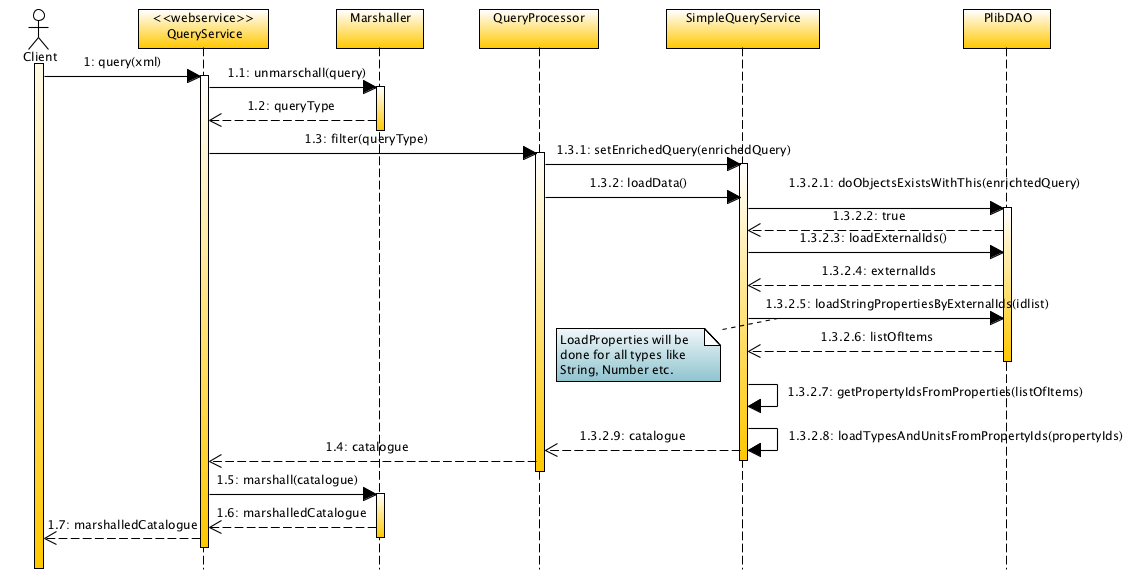
\includegraphics[width=0.99\textwidth]{images/plib_simple_query_sequence_diagram.png}
		\caption{Sequenzdiagramm Simple Query}
	\label{fig:sequenzdiagrammsimplequery}
\end{figure}




\section{Zusammenfassung des Kapitels}




%%\setchapterpreamble[u]{
%\dictum[Johann Wolfgang von Goethe]{Es ist nicht genug, zu wissen, man muß auch anwenden; es ist nicht genug, zu wollen, man muß auch tun. \dots}}
\section{Use Cases}\label{kap:Use_Cases} 
% Funktionale Anforderungen

Dieses Kapitel beschreibt mögliche Use Cases die sich aus ISO 29002-31 ergeben. 

Die Query-Code-Beispiele sind gekürzt, d.h. es werden beispielsweise referenzierte Schemata-Namen nicht aufgeführt. 

\begin{figure}[htbp]
	\centering
		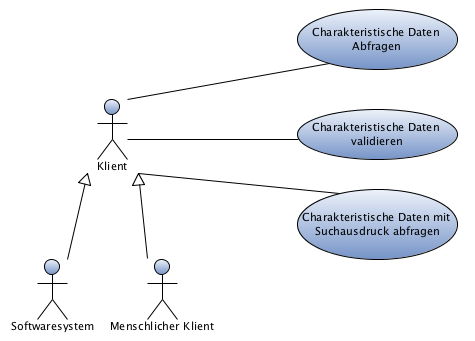
\includegraphics[width=0.75\textwidth]{images/usecases_plib.png}
	\caption{Use Case Übersicht}
	\label{fig:usecaseuebersicht}
\end{figure}

\subsection{Akteure}
Bei der Implementierung geht es um eine generische Schnittstelle. In den nachfolgenden Anwendungsfällen wird vom Akteur \enquote{Klient} gesprochen. Der Klient ist allgemein ein Nutzer der Schnittstelle, sei es als menschlicher Akteur welcher über eine Bedienerinterface die Schnittstelle benutzt oder eine direkte Maschinennutzung.    

%TODO Use Case Diagram

\subsection{Use Case Beschreibungen}

\subsubsection{Alle Charakteristische Daten eines Produkts abfragen}

{\small

\begin{description}
     \item[use case] Charakteristische Daten abfragen
     \item[  actors]~\\
     Klient
     \item[  precondition]~\\
     Der Klient verwendet einen gültigen Identifier.
     \item[  main flow]~\\
     Der Klient gibt einen Identifier (IRDI\footnote{International Registration Data Identifier}) einer Klasse von Elementen ein und sendet eine Anfrage ab. Die Anfrage wird auf Gültigkeit überprüft. Als Antwort bekommt er ein oder mehrere Datensätze von Elementen \footnote{Item, ISO 29002-10 Kapitel 5.3.2} mit den entsprechenden charakteristischen Daten \footnote{property\_values, ISO 29002-10 Kapitel 5.2.4}  des Elementes mit dem übergebenen Identifier zurück.
     \item[  postcondition]~\\
     Alle Daten aller Elemente der gewählten Klassen des Identifiers wurden zurückgegeben.    
     \item[  alternative flow] Properties auswählen ~\\
     Zusammen mit dem Identifier übergibt der Klient einen oder mehrere Property-Identifier und sendet diese erweiterte Anfrage ab.    
     \item[  postcondition]~\\
     Die mittels Property-Identifier ausgewählten Daten aller Elemente der gewählten Klassen wurden zurückgegeben.    
     \item[end] Charakteristische Daten abfragen
\end{description}

~\\

} %end small

\paragraph{Beispiel}

Ein Schraubendreher könnte folgendermaßen in einer Produktdatenbank repräsentiert werden:

\begin{description}\label{lab:schraubendreher}
\item[Klassen-Identifier] 0173-1\#01-AAA352\#4 
\item[Länge] 300mm
\item[Typ] Kreuz
\item[Spannungsfest] ja
\end{description}

Korrekterweise müssten anstatt der Attribute wie Länge oder Typ ebenfalls ein Identifier stehen. Die Benamungen sind hier zur besseren Lesbarkeit aufgelöst. 

Um nun alle Eigenschaften (Properties), wie Länge, Typ und Spannungsfest zu erhalten muss folgende Abfrage gesendet werden: 
\textbf{"Gib mir alle Items und alle Properties der Klasse mit dem Identifier 0173-1\#01-AAA352\#4 (Schraubendreher)".}
Das Ergebnis ist ein Item mit allen Attributen (Properties) der gewünschten Klassen und gegebenenfalls vorhandenen Unterklassen. In unserem Falle genau die oben angegebenen Werte.

Die XML-Abfrage sieht wie folgt aus:

\begin{lstlisting}[caption=Query Beispiel - Daten abfragen, language=XML, label=UseCaseDatenabfragen]
<?xml version="1.0" encoding="UTF-8"?>
<qy:query xsi:schemaLocation="...query query.xsd" xmlns:xsi="http://www.w3.org/2001/XMLSchema-instance" xmlns:cat="...catalogue" xmlns:val="...value" xmlns:qy="...query" xmlns:bas="...basic">
	<qy:class_ref>0173-1#01-AAA352#4</qy:class_ref>
</qy:query>
\end{lstlisting}

Eine Abfrage, welche die Properties der Klasse auswählt die zurückgeliefert werden sollen könnte lauten: 
\textbf{"Gib mir alle Items und die Properties Länge und Typ der Klasse mit dem Identifier 0173-1\#01-AAA352\#4 (Schraubendreher)".}
Das Ergebnis ist ein Item mit den gewünschten Attributen (Properties). 

Die XML-Abfrage:
\begin{lstlisting}[caption=Query Beispiel - Daten abfragen mit Propertyeinschränkung, language=XML, label=lst:UseCaseDatenabfragenProperty]

<?xml version="1.0" encoding="UTF-8"?>
<qy:query xsi:schemaLocation="...query query.xsd" xmlns:xsi="http://www.w3.org/2001/XMLSchema-instance" xmlns:cat="...catalogue" xmlns:val="...value" xmlns:qy="...query" xmlns:bas="...basic">
	<qy:class_ref>0173-1#01-AAA352#4</qy:class_ref>
	
	<!-- typ und laenge -->
	<qy:property_ref>0173-1#01-BBB111#1 0173-1#01-BBB222#1</qy:property_ref> 
	
</qy:query>
\end{lstlisting}

Listing \ref{lst:UseCaseDatenabfragenProperty} beinhaltet ein XML-Attribut property\_ref. Das wird mit gewünschten Property Identifier gefüllt, welche mit Leerzeichen getrennt werden. 

\subsubsection{Charakteristische Daten eines Produkts validieren}

{\small

\begin{description}
     \item[use case] Charakteristische Daten validieren
     \item[  actors]~\\
     Klient
     \item[  precondition]~\\
     Der Klient verwendet einen gültigen Identifier sowie auf den Identifier passende Daten..
     \item[  main flow]~\\
     Der Klient gibt einen Identifier eines Elementes (Klasse) ein. Zusätzlich übermittelt er zu diesem bekanntem Element Eigenschaften dieser Instanz des Elements und sendet eine Anfrage ab. Die Anfrage wird auf Gültigkeit überprüft. Als Antwort bekommt er ein oder mehrere Datensätze von Elementen mit den entsprechenden charakteristischen Daten zurück, auf welche die übergebenen Eigenschaften am besten zutreffen. 
     \item[  postcondition]~\\
     Alle Daten aller Elemente der gewählten Klassen des Identifiers werden zurückgegeben. Dies ermöglicht dem Klienten eine Validierung der ihm bereits bekannten Daten über ein Element. 
     \item[end] Charakteristische Daten validieren
\end{description}

~\\

} %end small

\paragraph{Beispiel}

In diesem Anwendungsfall verfügen wir bereits über Elemente/Wertenpaare einer bestimmten Klasse, z.B. eben jenen Schraubendreher

\textbf{"Ich habe hier ein mir bekanntes Item mit bestimmten Eigenschaften (Properties), Länge=300mm. Gib mir alle Items und alle Properties der Klasse mit dem Identifier 0173-1\#01-AAA352\#4 (Kreuzschraube) welche die mitgelieferten Eigenschaften haben".}
Das Ergebnis sind Items mit allen Properties der angegebenen Klasse, welche über die übergebenen Eigenschaften (Properties) verfügen. In unserem Fall vervollständigen wir unsere Properties mit den weiteren Properties "Typ" und "Spannungsfest".

Die XML-Abfrage sieht so aus:

\begin{lstlisting}[caption=Query Beispiel - Daten abfragen, language=XML, label=UseCaseDatenabfragen]
<?xml version="1.0" encoding="UTF-8"?>
<qy:query xsi:schemaLocation="...query query.xsd" xmlns:xsi="http://www.w3.org/2001/XMLSchema-instance" xmlns:cat="...catalogue" xmlns:val="...value" xmlns:qy="...query" xmlns:bas="...basic">
	<cat:item class_ref="0173-1#01-AAA352#4..">
		<cat:property_value property_ref="0173-1#01-BBB111#1">
			<val:integer_value></val:integer_value>
		</cat:property_value>
	</cat:item>
</qy:query>
\end{lstlisting}

\subsubsection{Chrarakteristische Daten mittels Suchausdruck abfragen }

{\small

\begin{description}
     \item[use case] Charakteristische Daten mit Suchausdruck abfragen
     \item[  actors]~\\
     Klient
     \item[  precondition]~\\
     Der Klient verwendet einen gültigen Identifier.
     \item[  main flow]~\\
     Der Klient gibt einen Identifier eines Elementes (Klasse) ein. Ferner übergibt er ein oder mehrere bekannte Property Identifier sowie passend dazu Werte zur Sucheinschränkung. 
     \item[  postcondition]~\\
     Alle Elemente auf jene diese Einschränkung der übergebenen Werte zutrifft wurden zurückgegeben. 
     \item[end] Charakteristische Daten mit Suchausdruck abfragen
\end{description}

~\\

} %end small

\paragraph{Beispiel}

Wir nehmen das Schraubendreher Beispiel aus \ref{lab:schraubendreher} zur Hand, und möchten eine Abfrage absenden, welche von der Klasse Schraubendreher alle Items erhalten soll die eine Länge zwischen 200 und 300 mm haben. 

Um nun alle Eigenschaften (Properties), wie Länge, Typ und Spannungsfest zu erhalten muss folgende Abfrage gesendet werden: 
\textbf{"Gib mir alle Items und alle Properties der Klasse mit dem Identifier 0173-1\#01-AAA352\#4 (Kreuzschraube)".}
Das Ergebnis ist ein Item mit allen Attributen (Properties) der gewünschten Klassen und gegebenenfalls vorhandenen Unterklassen. In unserem Falle genau die oben angegebenen Werte.

Die XML-Abfrage sieht so aus:

\begin{lstlisting}[caption=Query Beispiel - Daten abfragen, language=XML, label=UseCaseDatenabfragen]
<?xml version="1.0" encoding="UTF-8"?>
<qy:query xsi:schemaLocation="...query query.xsd" xmlns:xsi="http://www.w3.org/2001/XMLSchema-instance" xmlns:cat="...catalogue" xmlns:val="...value" xmlns:qy="...query" xmlns:bas="...basic">
	<qy:class_ref>0173-1#01-AAA352#4</qy:class_ref>
	<qy:characteristic_data_query_expression>
		<qy:range>
			<qy:property_reference property_ref="0173-1#01-BBB111#1"/>
			<qy:min_value>200</qy:min_value>
			<qy:max_value>300</qy:max_value>
			<qy:is_inclusive>true</qy:is_inclusive>
		</qy:range>
	</qy:characteristic_data_query_expression>
</qy:query>
\end{lstlisting}


%\section{Automatisierte Benutzerebene}
%Der Unterschied zur manuellen Benutzerebene ist der, dass hierbei automatisiert Daten angefragt und übermittelt werden. Es findet keine Mensch zu %Maschine Kommunikation statt sondern eine Maschine zu Maschine Kommunikation. 
%Ziel der automatisierten Anfragen ist das Abgleichen oder Validieren von Massendaten eines (Teil)-Katalogs. 

%\begin{description}
%\item[Alle Klassen abfragen] Der Klient sendet eine Anfrage und erhält alle vorhandene Klassen (ohne Items).
%\item[Items einer Klasse abgleichen] Der Klient möchte seine Daten abgleichen und fragt alle Items einer Klasse ab.  
%\item[Items einer Klasse validieren] Der Klient möchte seine Daten validieren und fragt alle Items einer Klasse ab.
%\end{description}
\chapter*{Schlussfolgerung und Ausblick in die Zukunft}

\addcontentsline{toc}{chapter}{Schlussfolgerung}

Die Zielsetzung dieser Arbeit, die Machbarkeit und Integration der ISO-Schnittstelle aufbauend auf die vorhandene PLIB-Datenbankimplementierung aufzuzeigen, wurde erreicht. Aktuelle Techniken und Frameworks ermöglichen eine relativ schnelle Integration der den Standards zugehörigen Schemata. Es lässt sich mit überschaubarem Aufwand ein Web Service erstellen. 
Es wurde aufgezeigt, dass im Rahmen der Abschlussarbeiten des Fachbereiches die Abfrageschnittstelle aufbauend auf die PLIB-Datenbank des Fachbereiches möglich ist. Während der Analyse und Implementierung ergaben sich einige Problemstellungen, die gelöst werden konnten. Beispielsweise ist die Heterogenität der Datenstrukturen ein nicht triviales Problem. Die Prozeduren konnten nicht direkt mit den von der Abfrage erhaltenen Daten aufgerufen werden. Es sind vorab Anfragen zur Transformation an die Datenbank nötig. 
Die zurückgelieferten Daten der Prozeduren liefern nicht alle Daten zurück die für das Füllen der XML-Katalog Daten nötig sind. Ferner passt die Struktur und Semantik der zurückgelieferten Daten nicht mit den Antwort des Standards überein. 
Dies konnte durch entsprechende Absprache unter den Studenten des Fachbereiches gelöst werden konnte. An den Prozeduren wurden keine umfangreichenden Änderungen durchgeführt, jedoch ermöglichten die Absprachen ein Verständnis, welches einen Lösungsweg ermöglichten. 

Die Umsetzung der Arbeit erfolgte mit Hilfe aktueller Technologien auf Basis von REST Web Services. Die Applikation kann automatisiert mit Hilfe eines Build Management Systems einfach erzeugt werden. Das ermöglicht es, dass andere Studenten das System ohne Aufwand erzeugen können. Die Quelltexte sind in einem Versionskontrollsystem abgelegt und ermöglichen anderen Studenten und Entwicklern den Zugriff darauf. 

Die Arbeit umfasst nicht die Implementierung einer GUI und ebenfalls nicht die Implementierung der Schnittstelle nach ISO 22745-30 Identification Guide. Dieser Standard beschreibt eine Möglichkeit, Regeln zu definieren, welche Konzepte (z.B aus PLIB) näher beschreiben. Das ermöglicht sinnvollerweise eine Einschränkung der Anfragedaten in der Form, wie es der Kunde respektive Klient in seinem Kontext benötigt. Man stelle sich vor, dass in einer Produktionsabteilung andere Daten von bestimmten Konzepten nötig sind als in der Verkaufsabteilung. Ein Beispiel wären bestimmte Eigenschaften des Materials über die Verformung bei großer Hitze in der Produktion. Bei einem Metall ist diese Information in der Produktion wichtig, da hier ggfs. hohe Hitzeentwicklung vorzufinden ist. Der Verkauf benötigt diese Informationen nicht oder nur gewisse Teile davon. Dies kann mit Hilfe von Identification Guides eingeschränkt werden. 
Als Folgearbeit wäre beispielsweise denkbar, die Implementierung von Identification Guides vorzunehmen. Um diese Einschränkung nach Regeln gemäß ISO 22745-30 zu demonstrieren könnte eine Benutzeroberfläche aus den Angaben generiert werden. Nehmen wir aus obigem Beispiel eine Applikation welche eine Benutzeroberfläche für die Abteilung Produktion und eine welche die Abteilung Verkauf repräsentiert. Diese könnten nach ISO 22745-30 unterschiedliche definierte Regelwerke besitzen und folglich eine andere Maske darstellen. Die Abfrage die somit von der Abteilung Produktion über die Maske gesendet werden kann, kann nur gewisse Eigenschaften eines Produktes abfragen die für die Abteilung relevant sind. Die Abfrage der Abteilung Verkauf kann folglich andere Eigenschaften abfragen die nur für diese Abteilung relevant sind.

Als mögliche weitere Arbeit wäre eine Gesamtintegration aller Arbeiten im Fachbereich denkbar. Diese könnte die Arbeiten von Herrn Mende, Herrn Loth, Frau Janßen und Herrn Sobek integrieren.  

\todotext{Folgenarbeiten beschreiben,  22745-30 zu implementieren, näher beschreiben warum und was da getan werden könnte, z.B. generierung der GUI aus dem Identification Guide Angaben der Produkte. Sinn: Vorauswahl beim Kunden, GUI wird generiert, dann Erzeugung query.xml nach 29002-31, wie in dieser Arbeit usw. Möglicherweise Gesamtintegration eine weitere Arbeit (Hr. Mende, Hr. Loth, Frau Janßen, Hr. Sobek; so könnte ein Praxisbeispiel komplett gezeigt werden, möglicherweise anhand eines simplen konkretem Beispiels.}
\chapter*{Eidesstattliche Erklärung}

Hiermit versichere ich, dass ich die vorliegende Arbeit selbstständig verfasst und keine anderen als die angegebenen Quellen und Hilfsmittel benutzt habe, dass alle Stellen der Arbeit, die wörtlich oder sinngemäß aus anderen Quellen übernommen wurden, als solche kenntlich gemacht und dass die Arbeit in gleicher oder ähnlicher Form noch keiner Prüfungsbehörde vorgelegt wurde.

\vspace{3cm}
Ort, Datum \hspace{5cm} Unterschrift (Stefan Sobek)\\

%%%%%%%%%%%%%%%%%%%%%%%%%%%%%%%%%%%%%%%%%%%%%%%%%%%%%%%%%%%%%
%% LITERATUR UND ANDERE VERZEICHNISSE
%%%%%%%%%%%%%%%%%%%%%%%%%%%%%%%%%%%%%%%%%%%%%%%%%%%%%%%%%%%%%
%% Ein kleiner Abstand zu den Kapiteln im Inhaltsverzeichnis (toc)
\addtocontents{toc}{\protect\vspace*{\baselineskip}}

%% Literaturverzeichnis

\addcontentsline{toc}{chapter}{Literaturverzeichnis}
%\nocite{*} %Auch nicht-zitierte BibTeX-Eintr‰ge werden angezeigt.
\bibliographystyle{alphadin}
%\bibliographystyle{plain}
\bibliography{literatur}


%%%%%%%%%%%%%%%%%%%%%%%%%%%%%%%%%%%%%%%%%%%%%%%%%%%%%%%%%%%%%
%% ANHÄNGEvi _
%%%%%%%%%%%%%%%%%%%%%%%%%%%%%%%%%%%%%%%%%%%%%%%%%%%%%%%%%%%%%
\appendix
\addcontentsline{toc}{chapter}{Anhang}

\chapter{Analyse ISO 29002-31 - Exchange of characteristics data}\label{kap:analyse2900231}

\section{XML Datencontaineranalyse ISO 29002-31}\index{ISO 29002-31}
Die Unterkapitel beschreiben die einzelnen (XML) Datencontainer aus der ISO 29002-31. Der Ausgangspunkt ist der query\_context, welcher einige Metadaten zum eigentlichen query enthält. 

\begin{figure}[htbp]
	\centering
		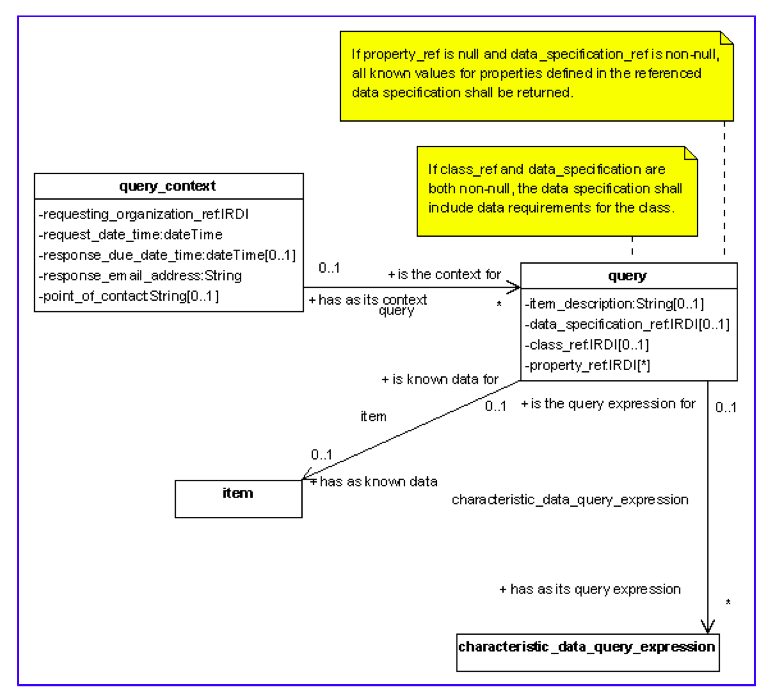
\includegraphics[width=0.99\textwidth]{images/query_main.png}
		\caption[UML-Diagramm Query Main]{UML-Diagramm Query Main\footnotemark}
	\label{fig:querymain}
\end{figure}
\footnotetext{Quelle: ISO 29002-31 Kapitel 5.2.1}

\subsection{query\_context}
Dies ist eine Art Container für eine Menge von Queries. Inhalt sind Informationen über den Anforderer der Daten zwecks persönlicher Kontaktaufnahme, wie z.B. die Anfragezeit, Informationen über die Organisation welche die Anfrage schickt sowie einen gewünschten Antwortzeitpunkt mit Antwort-Email Adresse. Siehe dazu \autoref{fig:querymain} und \citep[Kap. 5.2.2][]{iso29002-31}.  

Da die Vorgabe lautet, den Service auf Basis eines Web Services zu erstellen, entfällt die Benutzung des query\_context. Der Grund ist, dass der Kontext  implizit durch den Web Service respektive dem Server zur Verfügung gestellt wird. Beispielsweise wird die Anfragezeit zwar nicht explizit durch den Serviceaufrufer selbst übergeben, allerdings durch die Anfrage an den technischen Server wie z.B. Apache Tomcat Server mittels Logeintrag implizit ermittelt. Somit lassen sich diese Metadaten über Verbindungsprotokolle der Infrastruktur herausfinden.  
Siehe dazu auch \citep[Kap. 6][]{iso29002-31}, welche besagt: \\ \enquote{ISO/TS 29002 can be implemented: \\
a. with another envelope standard, such as EDI, or \\
b. by itself, using the query\_context to carry envelope information.}

\subsection{query}\label{sec:query}
Die Unterstützung aller Funktionalitäten des queries entspricht laut ISO 29002-31 der Conformance class 1: simple query \citep[Anhang 6][]{iso29002-31}.
Dies ist der eigentliche Abfrage-Datensatz. Abgefragt werden kann mittels class IRDI\footnote{IRDI  - International registration data identifier}, data\_specification IRDI, eine Menge von property IRDI, Teiledaten (das sind Teile gefüllt mit Daten ihrer Eigenschaften die dem Klienten bereits bekannt sind) und einer item\_description. Das bedeutet, dass bereits bekannte Eigenschaften eines Teils übertragen werden können, um die Suche auf Teile mit diesen Werte-Eigenschaften einzuschränken.

Die data\_specification IRDI verweist auf eine Spezifikation aus ISO 22745-30, die besagt welche Properties für dieses Teil sinnvoll sind. Die angegebenen Property IRDIs sind dann eine Teilmenge aus den mittels data\_specification IRDI definierten erlaubten Eigenschaften. Für weitere Informationen zur ISO 22745-30 siehe \autoref{kap:identification_guide_anhang}. 

Ad hoc denkbar wären einfache Abfragen wie z.B.: \enquote{Gib mir alle Teile der Klasse xyz}. Mitgeliefert werden auch Teile von Subklassen. Weiterhin kann die Abfrage nach bestimmten Eigenschaften eingeschränkt werden. Eine weitere Möglichkeit ist es bereits bekannte Daten über ein Element zu übermitteln, mit dem Zwecke hierüber die IRDI zu erfahren oder weitere Eigenschafts-Daten zu erhalten. Siehe Beispielqueries simple queries in \autoref{kap:query_beispiele}. 

\subsection{characteristic\_data\_query\_expression (parametric\_query)}\label{sec:characteristicdataqueryexpression}
Das entspricht laut ISO 29002-31 Anhang 6 der Conformance class 2: parametric query.

\begin{figure}[htbp]
	\centering
		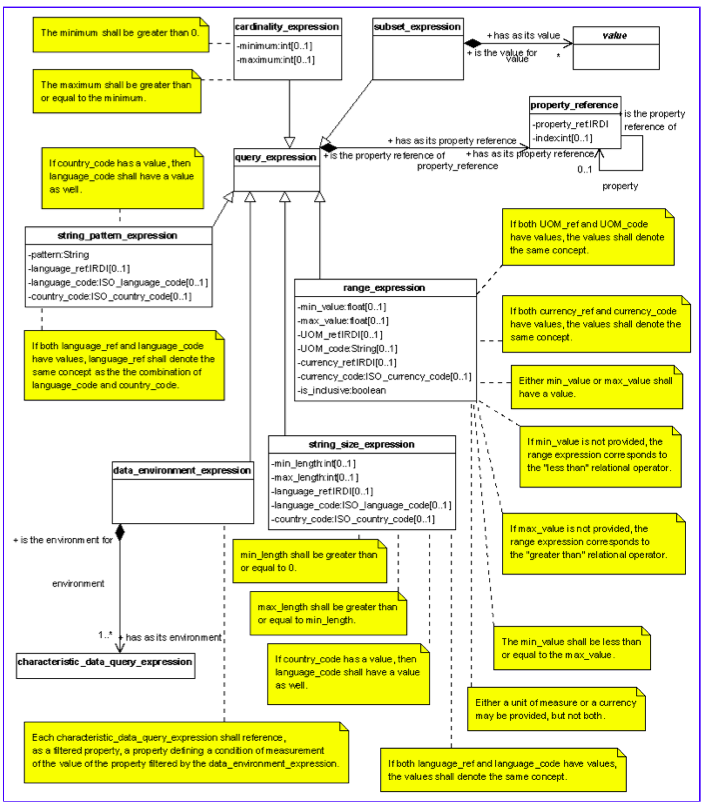
\includegraphics[width=0.99\textwidth]{images/query_expression.png}
		\caption[UML-Diagramm Query Expression]{UML-Diagramm Query Expression\footnotemark}
	\label{fig:umlqueryexpression}
\end{figure}
\footnotetext{Quelle: ISO 29002-31 Kapitel 5.3.1}

Eine characteristic\_data\_query\_expression kann verschieden expressions vom Typ query\_expression beinhalten. Von jedem Typ jeweils nur maximal eine. 
Z.B.
\begin{itemize}
\item string\_size\_expression
\item string\_pattern\_expression
\item range\_expression
\item data\_environment\_expression
\item cardinality\_expression
\item subset\_expression
\end{itemize}
darüberhinaus noch folgende Attribute

\begin{itemize}
\item property\_reference - die property auf den die query\_expression bezogen ist
\end{itemize}
Solch eine Expression ermöglicht das Filtern, gleichsam ein Einschränken bestimmter Properties und Werte. 

\subsection{Query Beispiele}\label{kap:query_beispiele}

Nachfolgend seien einige Query-Beispielszenarien aufgestellt, die sich aus der Analyse der Standards ergeben.

Eine Schraube hat die folgenden möglichen Eigenschaften: 

\begin{description}
\item[Klassen-Identifier] 1234-abcd\# ab-cdefgh\# 1 (IRDI)
\item[Typ] M6 (Property IRDI: 1234-abcd\# ab-bbbbbb\# 1)
\item[Länge] 80mm (Property IRDI: 1234-abcd\# ab-cccccc\# 1)
\end{description}

\subsubsection{Simple Query}\index{Query!Simple Query}

Ein simpler query ermöglicht folgende Abfrage: \enquote{Gib mir alle Teile zum Konzept Kreuzschraube mit dem Identifier (IRDI) 1234-abcd\#ab-cdefgh\#1}. Das Ergebnis ist ein Teil, mit allen Attributen wie oben angegeben. 

Ein anderer Query könnte lauten: \enquote{Gib mir die Properties 1234-abcd\#ab-cccccc\#1 und 1234-abcd\#bbbbbb\# 1 des Items der Klasse 1234-abcd\#ab-cdefgh\#1}. Das Ergebnis wäre das Teil mit Typ: M6 und der Länge: 80mm.

Es könnte auch mit Hilfe von vorhandenen Daten gesucht werden, z.B.:  \enquote{Hier ist ein Teil mit der Property Typ: M6 (Property IRDI: 1234-abcd\# ab-bbbbbb\# 1), gib mir bitte dazu die Properties 1234-abcd\#ab-cccccc\#1 und 1234-abcd\# bbbbbb\#1} 

\subsubsection{Parametric Query}\index{Query!Parametric Query}

Hat man jetzt noch eine Schraube mit folgenden Eigenschaften:
\begin{description}
\item[Klassen-Identifier] 1234-abcd\#ab-cdefgh\#1 (IRDI)
\item[Typ] M5 (Property IRDI: 1234-abcd\#xx-bbbbbb\#1)
\item[Länge] 100mm (Property IRDI: 1234-abcd\#xx-cccccc\#1)
\end{description}

ermöglicht der Parametric Query mit Hilfe der characteristic\_data\_query\_expression folgende Abfragen:  \enquote{Gib mir die Properties 1234-abcd\# ab-cccccc\#1 (Länge) und 1234-abcd\#bbbbbb\#1 (Typ) des Konzeptes 1234-abcd\#ab-cdefgh\#1 (Schraube) mit einer Länge zwischen 50 und 150mm und dem Typen M5 oder M6.}

Dies ermöglicht das Filtern auf genau eine übergebene Property. Rekursive Abfragen sind auch möglich, beispielsweise wenn die gesuchte Property eine Multi-Property ist (Property: Loch als Wert zwei Properties mit Form und Durchmesser und Durchmesser soll gefiltert werden)

\section{Analyse ISO 22745-30 - Identification Guide}\label{kap:identification_guide_anhang}\index{ISO 22745-30}

\todotext{Quelle für i-xml file aus eotd-i-xml angeben} 
Ein Identification Guide beschreibt, welche Daten für ein Objekt benötigt werden, damit dies überhaupt sinnvoll für einen bestimmten Zweck eingesetzt werden kann. Der Käufer, Produktmanager oder Benutzer definiert die Anforderungen an die Daten. Ein  \enquote{Datenanforderungsstatement} wird als ein i-xml identification guide xml file erzeugt. Es wird definiert, was der Name des Artikels ist mit den charakteristischen Daten. Es wird die Frage beantwortet, welche Daten (Properties) zu einem bestimmten Konzept eines Objektes benötigt werden um den Artikeln zu kaufen oder zu sinnvoll zu verwalten. Diese Anforderungen werden von der Abfrageseite (Kundenseite) definiert, also derjenige, der Daten abfragen möchte. \(Quelle: ECCMA\_ISO\_8000\_certification.pdf\) \todotext{Quelle sauber in library file verlinken}
Ein Identification guide referenziert Konzepte eines Dictionaries um Datenanforderungen einer bestimmten Klasse zu beschreiben. (ISO 22745-30 Kapitel 5). 
Ein Datenempfänger kann eine Organisation oder eine Gruppe von Organisationen oder Firmen sein, welche ähnliche Datenanforderungen haben. Somit wird eine Identification Guide Gruppe von einer speziellen Organisation verwaltet, welche wiederum selbst Datenempfänger sein kann.  


%\setchapterpreamble[u]{
%\dictum[Johann Wolfgang von Goethe]{Es ist nicht genug, zu wissen, man muß auch anwenden; es ist nicht genug, zu wollen, man muß auch tun. \dots}}
\chapter{Anwendungsfälle}\label{kap:analyse_use_cases}
% Funktionale Anforderungen

Dieses Kapitel beinhaltet weiteren Anwendungsfälle des Systems. Der in \autoref{kap:Use_Cases} bereits beschriebenen Anwendungsfall wird hier nicht erneut aufgeführt.  

\subsection{Charakteristische Daten eines Produkts validieren}

{\small

\begin{description}
     \item[use case] Charakteristische Daten validieren
     \item[  actors]~\\
     Klient
     \item[  precondition]~\\
     Der Klient verwendet einen gültigen Identifier sowie auf den Identifier passende Daten..
     \item[  main flow]~\\
     Der Klient gibt einen Identifier eines Elementes (Klasse) ein. Zusätzlich übermittelt er zu diesem bekanntem Element Eigenschaften dieser Instanz des Elements und sendet eine Anfrage ab. Die Anfrage wird auf Gültigkeit überprüft. Als Antwort bekommt er ein oder mehrere Datensätze von Elementen mit den entsprechenden charakteristischen Daten zurück, auf welche die übergebenen Eigenschaften am besten zutreffen. 
     \item[  postcondition]~\\
     Alle Daten aller Elemente der gewählten Klassen des Identifiers werden zurückgegeben. Dies ermöglicht dem Klienten eine Validierung der ihm bereits bekannten Daten über ein Element. 
     \item[end] Charakteristische Daten validieren
\end{description}

~\\

} %end small

\subsubsection{Beispiel}

In diesem Anwendungsfall verfügen wir bereits über Elemente/Wertepaare eines bestimmten Konzeptes, z.B. eben jenen Schraubendreher.

\enquote{Ich habe hier ein mir bekanntes Item mit bestimmten Eigenschaften (Properties), Länge=300mm. Gib mir alle Items und alle Properties der Klasse mit dem Identifier 0173-1\#01-AAA352\#4 (Kreuzschraube) welche die mitgelieferten Eigenschaften haben.}
Das Ergebnis sind Teile mit allen Properties des angegebenen Konzeptes, welche über die übergebenen Eigenschaften (Properties) verfügen. In unserem Fall vervollständigen wir unsere Properties mit den weiteren Properties \enquote{Typ} und \enquote{Spannungsfest}.

Die XML-Abfrage gemäß query.xsd\footnote{Schema Datei ist referenziert in ISO 29002-31, liegt der Arbeit bei} sieht so aus:

\begin{lstlisting}[caption=Query Beispiel - Daten validieren, language=XML, label=UseCaseDatenvalidieren]
<?xml version="1.0" encoding="UTF-8"?>
<qy:query xsi:schemaLocation="...query query.xsd" xmlns:xsi="http://www.w3.org/2001/XMLSchema-instance" xmlns:cat="...catalogue" xmlns:val="...value" xmlns:qy="...query" xmlns:bas="...basic">
	<cat:item class_ref="0173-1#01-AAA352#4..">
		<cat:property_value property_ref="0173-1#01-BBB111#1">
			<val:integer_value></val:integer_value>
		</cat:property_value>
	</cat:item>
</qy:query>
\end{lstlisting}

\subsection{Chrarakteristische Daten mittels Suchausdruck abfragen }

{\small

\begin{description}
     \item[use case] Charakteristische Daten mit Suchausdruck abfragen
     \item[  actors]~\\
     Klient
     \item[  precondition]~\\
     Der Klient verwendet einen gültigen Identifier.
     \item[  main flow]~\\
     Der Klient gibt einen Identifier eines Konzeptes ein. Ferner übergibt er ein oder mehrere bekannte Property Identifier sowie passend dazu Werte zur Sucheinschränkung. 
     \item[  postcondition]~\\
     Alle Elemente auf jene diese Einschränkung der übergebenen Werte zutrifft wurden zurückgegeben. 
     \item[end] Charakteristische Daten mit Suchausdruck abfragen
\end{description}

~\\

} %end small

\subsubsection{Beispiel}

Wir nehmen das Schraubendreher Beispiel aus \autoref{lab:schraubendreher} zur Hand, und möchten eine Abfrage absenden, welche von der Klasse Schraubendreher alle Items erhalten soll die eine Länge zwischen 200 und 300 mm haben. 

Um nun alle Eigenschaften (Properties), wie Länge, Typ und Spannungsfest zu erhalten muss folgende Abfrage gesendet werden: 
\enquote{Gib mir alle Items und alle Properties der Klasse mit dem Identifier 0173-1\#01-AAA352\#4 (Kreuzschraube).}
Das Ergebnis ist ein Item mit allen Attributen (Properties) der gewünschten Klassen und gegebenenfalls vorhandenen Unterklassen. In unserem Falle genau die oben angegebenen Werte.

Die XML-Abfrage gemäß query.xsd\footnote{Schema Datei ist referenziert in ISO 29002-31, liegt der Arbeit bei} sieht so aus:

\begin{lstlisting}[caption=Query Beispiel - Daten mit Suchausdruck abfragen, language=XML, label=UseCaseDatenabfragen]
<?xml version="1.0" encoding="UTF-8"?>
<qy:query xsi:schemaLocation="...query query.xsd" xmlns:xsi="http://www.w3.org/2001/XMLSchema-instance" xmlns:cat="...catalogue" xmlns:val="...value" xmlns:qy="...query" xmlns:bas="...basic">
	<qy:class_ref>0173-1#01-AAA352#4</qy:class_ref>
	<qy:characteristic_data_query_expression>
		<qy:range>
			<qy:property_reference property_ref="0173-1#01-BBB111#1"/>
			<qy:min_value>200</qy:min_value>
			<qy:max_value>300</qy:max_value>
			<qy:is_inclusive>true</qy:is_inclusive>
		</qy:range>
	</qy:characteristic_data_query_expression>
</qy:query>
\end{lstlisting}


%\section{Automatisierte Benutzerebene}
%Der Unterschied zur manuellen Benutzerebene ist der, dass hierbei automatisiert Daten angefragt und übermittelt werden. Es findet keine Mensch zu %Maschine Kommunikation statt sondern eine Maschine zu Maschine Kommunikation. 
%Ziel der automatisierten Anfragen ist das Abgleichen oder Validieren von Massendaten eines (Teil)-Katalogs. 

%\begin{description}
%\item[Alle Klassen abfragen] Der Klient sendet eine Anfrage und erhält alle vorhandene Klassen (ohne Items).
%\item[Items einer Klasse abgleichen] Der Klient möchte seine Daten abgleichen und fragt alle Items einer Klasse ab.  
%\item[Items einer Klasse validieren] Der Klient möchte seine Daten validieren und fragt alle Items einer Klasse ab.
%\end{description}
\chapter{Installationsanleitung Apache Tomcat 7}\label{kap:anhangtomcat}

\section{Installation auf Mac OS 10.8}

Diese Installationsanleitung bezieht sich auf die Installation des Apache Tomcat 7 in Mac OS 10.8. 

\subsection{Prüfen der Java Version}

Mittels 

\lstinline[basicstyle=\ttfamily\small\mdseries]{java -version}

prüfen, ob Version 1.6 oder 1.7 installiert ist. Falls nicht, muss Java vorher installiert werden. Dazu das Java Development Kit herunterladen und installieren: \href{http://www.oracle.com/technetwork/java/javase/overview/index.html}{http://www.oracle.com/technetwork/java/javase/overview/index.html}

Für den Mac ist das ggf. über die Apple-Webseite verfügbar. 

\subsection{Tomcat herunterladen und entpacken}

\begin{itemize}
\item Auf \href{https://tomcat.apache.org/download-70.cgi}{https://tomcat.apache.org/download-70.cgi} Tomcat herunterladen. Darauf achten eine Binary distribution herunterzuladen, z.B. apache-tomcat-7.0.42.tar.gz
\item Das Paket entpacken mittels tar -xvzf apache-tomcat-7.0.42.tar.gz
\end{itemize}

\begin{itemize}
\item Ein Verzeichnis unter \href{file:///usr/local}{/usr/local} erstellen, wo der Apache später laufen soll, danach die Dateien dort hinkopieren
\begin{itemize}
	\item sudo mkdir -p \href{file:///usr/local}{/usr/local}
	\item sudo mv \href{file:///Users/stefan/Downloads/apache-tomcat-7.0.42}{~/Downloads/apache-tomcat-7.0.42} \href{file:///usr/local}{/usr/local/}
\end{itemize}\item Einen symbolischen Link erstellen um später einfacherer zwischen Versionen umzuschalten:
\begin{itemize}
	\item sudo rm -f \href{file:///Library/Tomcat}{/Library/Tomcat}
	\item sudo ln -s \href{file:///usr/local/apache-tomcat-7.0.42}{/usr/local/apache-tomcat-7.0.42} \href{file:///Library/Tomcat}{/Library/Tomcat}
\end{itemize}\item Allen Apache Dateien den aktuellen User als Besitzer setzen und Rechte vergeben:
\begin{itemize}
	\item sudo chown -R \textless{}dein\_username\textgreater{} \href{file:///Library/Tomcat}{/Library/Tomcat}
	\item sudo chmod +x \href{file:///Library/Tomcat/bin/*.sh}{/Library/Tomcat/bin/*.sh}
\end{itemize}\end{itemize}

\subsection{Tomcat starten}

\href{file:///Library/Tomcat/bin/startup.sh}{/Library/Tomcat/bin/startup.sh}

\subsection{Tomcat stoppen}

\href{file:///Library/Tomcat/bin/shutdown.sh}{/Library/Tomcat/bin/shutdown.sh}

\section{Installation unter Windows}

Am besten wird der Tomcat mittels Installer installiert. Hier wird man durch eine grafische Benutzeroberfläche geführt und Apache Tomcat wird als Dienst in das System integriert. 

\section{Tomcat mittels Maven starten}

Um Tomcat mittels Maven zu starten, muss Tomcat als Plugin in der Maven \gls{pom} konfiguriert werden. Das \autoref{lst:tomcat_plugin} zeigt die Konfiguration für die \gls{pom}.

 \begin{lstlisting}[caption=Tomcat 7 Maven Plugin, language=XML, label=lst:tomcat_plugin]
<build>
  <plugins>
    <plugin>
      <groupId>org.apache.tomcat.maven</groupId>
      <artifactId>tomcat7-maven-plugin</artifactId>
    </plugin>
  </plugins>
</build>
 \end{lstlisting}  
 
Anschließend kann der Tomcat-Server mit folgendem Befehl gestartet werden:
 
\lstinline[basicstyle=\ttfamily\small\mdseries]{mvn tomcat7:run}
 

 


\chapter{Automatische Entwicklertests} \index{JUnit}\label{anh:automatischeentwicklertests}
 
\section{Unit Test}\index{Unit Test}
Nachfolgend ein Beispiel eines Unit Tests. Das Testobjekt ist die Klasse XMLMarshaller, welcher für das \gls{Marshalling} und \gls{Unmarshalling} der XML-Daten verantwortlich ist. Hinweis: Alle Quelltexte verzichten auf import- und package-Anweisungen um die Lesbarkeit zu erhöhen. Die Original Quelltexte liegen der Arbeit bei. 
 
\begin{lstlisting}[caption=Beispiel eines Unit Tests, language=XML, label=lst:unittest_beispiel]
package de.feu.plib.xml;

/**
 * Tests the marshalling and unmarshalling of xml files.
 */
public class XMLMarshallerTest extends AbstractXMLTest {

    /** XML Marshaller instance under test */
    XMLMarshaller marshaller;

    /** Logger instance */
    private static final Logger LOGGER = Logger.getLogger(XMLMarshallerTest.class);

    /**
     * Simple marshalling test with arbitrary catalogue item.
     */
    @Test
    public void testMarshallingWithValidArbitraryCatalogue() {
        String catalogue = marshaller.marshall(createCatalogueWithOneItem());
        LOGGER.info(catalogue);
        assertTrue(catalogue.contains("0173-1#01-AAA352#4"));
        assertTrue(catalogue.contains("true"));
    }

    /**
     * Simple test with unmarshalling an arbitrary item from xml.
     */
    @Test
    public void testUnMarshallingWithValidArbitraryClassIrdi() {
        QueryType queryType = marshaller.unmarshallXML(readXMLFrom("/de/feu/plib/xml/query_class_irdi.xml"),
                QueryType.class);
        assertEquals("0173-1#01-BAD803#2", queryType.getClassRef());
    }

    /**
     * Throws an exception while parsing on illegal irdi passed.
     *
     * @throws Exception on illegal irdi
     */
    @Test(expected = RuntimeException.class)
    public void shouldThrowExceptionDuringXMLValidationWithIllegalIrdi() throws Exception {
        QueryType queryType = marshaller.unmarshallXML(readXMLFrom("/de/feu/plib/xml/query_class_irdi_illegal.xml"),
                QueryType.class);
    }

    /**
     * creates a sample catalogue for testing
     * 
     * @return the sample catalogue with one item
     */
    private CatalogueType createCatalogueWithOneItem() {
        ItemType item = new ItemType();
        item.setClassRef("0173-1#01-AAA352#4");
        PropertyValueType propertyValueType = new PropertyValueType();

        BooleanValueType bvt = new BooleanValueType();
        bvt.setValue(true);
        propertyValueType.setBooleanValue(bvt);
        propertyValueType.setPropertyRef("0173-1#01-A35AA2#4");
        item.getPropertyValue().add(propertyValueType);
        CatalogueType catalogue = new CatalogueType();
        catalogue.getItem().add(item);

        return catalogue;
    }

    /**
     * @throws java.lang.Exception
     */
    @Before
    public void setUp() {
        marshaller = new XMLMarshallerImpl();
    }

    /**
     * @throws java.lang.Exception
     */
    @After
    public void tearDown() {
        marshaller = null;
    }

}
\end{lstlisting}  

Das \autoref{lst:abstrakte_unit_testklasse} zeigt die abstrakte Klasse \enquote{AbstractXMLTest}, welche Hilfsmethoden für XML-Tests kapselt. Hier kapselt diese Klasse die Funktionalität XML-Dateien einzulesen.  

\begin{lstlisting}[caption=Abstrakte Unit Testklasse, language=Java, label=lst:abstrakte_unit_testklasse]

/**
 * Abstract test class. Extend from this class to get functionality to read XML files for your test.
 */
public class AbstractXMLTest {

    protected XMLMarshaller marshaller;

    /**
     * Logger instance
     */
    private static Logger LOGGER = Logger.getLogger(AbstractXMLTest.class);

    @Before
    public void setUp() {
        marshaller = new XMLMarshallerImpl();
    }

    @After
    public void tearDown() {
        marshaller = null;
    }

    /**
     * Reads the xml file from given filename
     *
     * @param filename the filename of the xml
     * @return the string content of the xml file
     */
    protected String readXMLFrom(String filename) {
        BufferedReader br = null;
        StringBuffer sb = new StringBuffer();

        try {
            String currentLine;

            InputStream is = XMLMarshallerImpl.class.getResourceAsStream(filename);
            br = new BufferedReader(new InputStreamReader(is));

            while ((currentLine = br.readLine()) != null) {
                sb.append(currentLine);
            }

        } catch (IOException e) {
            e.printStackTrace();
        } finally {
            try {
                if (br != null) br.close();
            } catch (IOException ex) {
                LOGGER.info("Exception occured during reading file: " + ex);
            }
        }

        return sb.toString();
    }
}
\end{lstlisting}  

\section{Integrationstest}\index{Integrationstest}

Dieser Abschnitt zeigt beispielhaft einen Integrationstest auf. Der Integrationstest unterscheidet sich vom Unit-Test darin, dass eine Komponente integriert mit mehreren abhängigen Komponenten getestet wird. 
Der nachfolgende Integrationstestfall \enquote{PlibDaoIT} aus \autoref{lst:integrationstest_beispiel} testet die Klasse \enquote{PlibDao}. Es ist ein Integrationstest, da für den Test die gesamte Datenbank benötigt wird. Nur so kann sinnvoll das Datenzugriffsobjekt getestet werden. 

Gestartet werden kann der Integrationstest mit Maven mittles Aufruf von 

\lstinline[basicstyle=\ttfamily\small\mdseries]{mvn integration-test}

\begin{lstlisting}[caption=Beispiel eines Integrationstests, language=Java, label=lst:integrationstest_beispiel]

/**
 * Integration Test of PLIB Dao
 */
@RunWith(SpringJUnit4ClassRunner.class)
@ContextConfiguration(locations = {"/beans_for_tests.xml"})
public class PlibDaoIT {

    /**
     * Logger instance
     */
    private static Logger LOGGER = Logger.getLogger(PlibDaoIT.class);

    @Autowired
    private PlibDao plib;

    @Test
    public void shouldReturnTrueWithExistingIRDI() {
        Irdi irdi = createMultiListTestIrdi();
        assertTrue(plib.doObjectsExistsWithThis(irdi));
    }

    @Test
    public void shouldReturnFalseWithIRDINotinDB() {
        Irdi irdi = createNonExistingTestIrdi();
        assertFalse(plib.doObjectsExistsWithThis(irdi));
    }

    @Test
    public void shouldReturnFalseWithEmptyIRDI() {
        Irdi irdi = new Irdi() {
            @Override
            public String getIrdi() {
                return "";
            }
        };
        assertFalse(plib.doObjectsExistsWithThis(irdi));
    }

    @Test
    public void testGetNumberOfObjectsOfIrdiExistingIrdi() {
        Irdi irdi = createMultiListTestIrdi();
        assertEquals(8, plib.getNumberOfObjectsOfIrdi(irdi));
    }

    @Test
    public void testGetNumberOfObjectsOfIrdiNotExistingIrdi() {
        Irdi irdi = createNonExistingTestIrdi();
        assertEquals(0, plib.getNumberOfObjectsOfIrdi(irdi));
    }

    @Test
    public void testThatWhenReadExternalProductIdsByIrdiMustReturnSome() throws Exception {
        Irdi irdi = createMultiListTestIrdi();
        List<BigDecimal> productIds = plib.readExternalProductIdsBy(irdi);
        assertNotNull(productIds);
        assertEquals(8, productIds.size());
    }

    /**
     * Currently there are two instances in the database, seems that these are duplicates but not sure.
     */
    @Test
    public void shouldReturnOneTestExternalIdWithTestIrdi() {
        Irdi irdi = createSkalpellIrdi();
        List<BigDecimal> externalProductIds = plib.readExternalProductIdsBy(irdi);
        assertNotNull(externalProductIds);
        assertEquals(2, externalProductIds.size());
        LOGGER.info("external product ids: " + externalProductIds.get(0));
        assertEquals(new BigDecimal("300000001"), externalProductIds.get(0));
    }

    /**
     * This is a bigger integration test.
     * <ul>
     *     <li>First create an irdi instance</li>
     *     <li>create an enriched query</li>
     *     <li>Then load the objects from the database with its properties</li>
     *     <li>There should be the same number ob objects than with the previous check</li>
     * </ul>
     */
    @Test
    @Ignore("loadObjectsFrom is obsolte, maybe later reimplemented")
    public void shouldReturnOneInstanceOfSkalpellWithTwoProperties() {
        Irdi skalpellIrdi = createSkalpellIrdi();

        List<BigDecimal> externalProductIds = plib.readExternalProductIdsBy(skalpellIrdi);

        EnrichedQuery query = createEnrichedQueryFrom(skalpellIrdi);
        query.setType(QueryKind.SIMPLE);
        CatalogueType catalogueType = plib.loadObjectsFrom(query);
        List<ItemType> itemTypes = catalogueType.getItem();
        assertEquals(externalProductIds.size(), itemTypes.size());
        assertEquals(1, itemTypes.get(0).getPropertyValue().size());
    }

    /**
     * Test should return two items where the first one would be checked.
     * Should have two properties.
     */
    @Test
    public void testLoadPropertiesByExternalIds() {
        List<BigDecimal> externalIds = new ArrayList<BigDecimal>();
        BigDecimal bigDecimal = new BigDecimal("300000001");

        externalIds.add(bigDecimal);
        List<List<Map<String, Object>>> valueTypeList = plib.loadStringPropertiesByExternalIds(externalIds);
        LOGGER.info("valuetype list: " + valueTypeList);
        assertEquals("should be one instance", 1, valueTypeList.size());
        assertEquals("should be two properties",2, valueTypeList.get(0).size());
        assertThatIrdiAndValueAreAvailable(valueTypeList.get(0).get(0).entrySet(), "0173-1#02-AAA762#1");
        assertThatIrdiAndValueAreAvailable(valueTypeList.get(0).get(1).entrySet(), "0173-1#02-AAB011#1");
    }

    private void assertThatIrdiAndValueAreAvailable(Set<Map.Entry<String, Object>> entrySet, String knownIRDI) {

        Set<Map.Entry<String, Object>> entries = entrySet;
        boolean irdiFound = false;
        boolean valueFound = false;
        for (Map.Entry<String, Object> entry : entries) {
            LOGGER.info("key of property: " + entry.getKey());
            LOGGER.info("value of property: " + entry.getValue());
            if ("IRDI".equals(entry.getKey()) && null != entry.getValue() && !"null".equals(entry.getValue())) {
                irdiFound = true;
                assertEquals(knownIRDI, entry.getValue());
            }
            if ("VALUE".equals(entry.getKey()) && null != entry.getValue() && !"null".equals(entry.getValue())) {
                valueFound = true;
            }

        }
        assertTrue(irdiFound && valueFound);
    }

    /**
     * Load data type and unit for skalpell length property which should be mm and mm as well.
     * Property id: 300903090000033914 and 300903090000034450
     */
    @Test
    public void testLoadDataTypeAndUnitForAPropertyById() {
        List<Map<String, Object>> propertyTypeAndUnit = plib.loadTypeAndUnitOfPropertyBy("300903090000033914");
        LOGGER.info("property size: " + propertyTypeAndUnit.size());
        assertTrue(propertyTypeAndUnit.size() == 1);

        assertThatUnitAndSubTypeAreAvailable(propertyTypeAndUnit);

    }

    private void assertThatUnitAndSubTypeAreAvailable(List<Map<String, Object>> propertyTypeAndUnit) {
        Set<Map.Entry<String,Object>> entries = propertyTypeAndUnit.get(0).entrySet();

        /*
        * we need to assure that we have the unit (in this case SYMBOL, e.g. mm or m or cm)
        * in the values as well as the type of the value (in this case real_measure_type)
        */
        String property_unit_symbol = "SYMBOL";
        String property_type = "SUB_TYPE";
        boolean unitfound = false;
        boolean typefound = false;
        for (Map.Entry<String, Object> entry : entries) {
            LOGGER.info("property key: " + entry.getKey());
            LOGGER.info("property value: " + entry.getValue());
            if ("SYMBOL".equals(entry.getKey()) && null != entry.getValue() && !"null".equals(entry.getValue())) {
                unitfound = true;
            }
            if ("SUB_TYPE".equals(entry.getKey()) && null != entry.getValue() && !"null".equals(entry.getValue())) {
                typefound = true;
            }
        }
        assertTrue(unitfound && typefound);
    }

    private EnrichedQuery createEnrichedQueryFrom(Irdi skalpellIrdi) {
        QueryType queryType = new QueryType();
        queryType.setClassRef(skalpellIrdi.getIrdi());
        return new EnrichedQuery(queryType);
    }

    private Irdi createNonExistingTestIrdi() {
        return new Irdi() {
            @Override
            public String getIrdi() {
                return "0141-1#01-xxx#1";
            }
        };
    }

    private Irdi createMultiListTestIrdi() {
        return new Irdi() {
            @Override
            public String getIrdi() {
                return "0141-1#01-UKU1#1";
            }
        };
    }

    /**
     * Creates the irdi of an item which was created by me as testdata.
     * It is a Skalpell (PREFERRED_NAME of class in DB)
     * @return the irdi of the test item skalpell.
     */
    private Irdi createSkalpellIrdi() {
        return new Irdi() {
            @Override
            public String getIrdi() {
                return "0173-1#01-BAD803#2";
            }
        };
    }
}

\end{lstlisting}  
   
\chapter{Testszenarios und Testtools} \index{Testszenarios}\index{Manuelle Entwicklertests}\label{anh:testszenarios}

Anbei die Testprotokolle der manuellen Entwicklertests.

Diese können mit den in \autoref{anh:testtools} aufgeführen Testtools oder alternativ mit der Testbenutzeroberfläche durchgeführt werden. Diese ist erreichbar unter: \\~
http://localhost:8080/plib-characteristic-query/query.xhtml

\section{Simple query}

\subsection{Vorhandene Teile anhand IRDI abfragen}

Es wird eine IRDI übermittelt.

\begin{description}
\item[Vorbedingungen] 
  \begin{itemize}
   \item Die Datenbankverbindung aufbauen: Oracle Datenbank muss gestartet werden.
  \end{itemize}
\item[Eingabedaten] Testdatei simple\_query\_irdi.xml. 
\item[Durchführung]
   \begin{itemize}
   \item XML-Datei wird mittels curl Befehl an den Server gesendet.
   \item curl -v -H 'Content-Type: application/xml' -X POST --data '@simple\_query\-\_irdi.xml' http://localhost:8080/plib-characteristic-query/rest/ws/query
  \end{itemize}
\item[Erwartetes Ergebnis] Zwei Items mit je zwei Eigenschaften werden erwartet. 
\item[Tatsächliches Ergebnis] Zwei Items mit zwei Eigenschaften.
\item[OK/Nicht OK?] OK
\end{description}


\subsection{Ungültige IRDI angegeben}

Es wird eine ungültige IRDI (gemäß XSD ungültig) übermittelt. 

\begin{description}
\item[Vorbedingungen] 
  \begin{itemize}
   \item Die Datenbankverbindung aufbauen: Oracle Datenbank muss gestartet werden.
  \end{itemize}
\item[Eingabedaten] Testdatei simple\_query\_illegal\_irdi.xml. 
\item[Durchführung]
   \begin{itemize}
   \item XML-Datei wird mittels curl Befehl an den Server gesendet.
   \item curl -v -H 'Content-Type: application/xml' -X POST --data \\ 
   '@simple\_query\_illegal\_irdi.xml' \\
   http://localhost:8080/plib-characteristic-query/rest/ws/query
  \end{itemize}
\item[Erwartetes Ergebnis] Fehlermeldung
\item[Tatsächliches Ergebnis] Fehlermeldung, marshalling error
\item[OK/Nicht OK?] OK
\end{description}

\subsection{Vorhandene Teile anhand IRDI abfragen mit Projektion}

Es wird eine IRDI übermittelt und zusätzlich eine Projektion (Eigenschaftsauswahl) vorgenommen.

\begin{description}
\item[Vorbedingungen] 
  \begin{itemize}
   \item Die Datenbankverbindung aufbauen: Oracle Datenbank muss gestartet werden.
  \end{itemize}
\item[Eingabedaten] Testdatei simple\_query\_projection\_one\_property.xml. 
\item[Durchführung]
   \begin{itemize}
   \item XML-Datei wird mittels curl Befehl an den Server gesendet.
   \item curl -v -H 'Content-Type: application/xml' -X POST --data \\
   '@simple\_query\_projection\_one\_property.xml' \\
   http://localhost:8080/plib-characteristic-query/rest/ws/query
  \end{itemize}
\item[Erwartetes Ergebnis] Zwei Items mit je einer Property, die angefragte Eigenschaft wird zurückgegeben. 
\item[Tatsächliches Ergebnis] Zwei Items mit einer Property. 
\item[OK/Nicht OK?] OK
\end{description}


\subsection{Vorhandene Teile mit bekannten Werten validieren}

Es wird eine IRDI übermittelt und zusätzlich Werte dieses Items übermittelt. Diese sollen validiert werden. Es wird dabei geprüft ob die Werte auch so in der Datenbank vorhanden. 

\begin{description}
\item[Vorbedingungen] 
  \begin{itemize}
   \item Die Datenbankverbindung aufbauen: Oracle Datenbank muss gestartet werden.
  \end{itemize}
\item[Eingabedaten] Testdatei simple\_query\_validation.xml. 
\item[Durchführung]
   \begin{itemize}
   \item XML-Datei wird mittels curl Befehl an den Server gesendet.
   \item curl -v -H 'Content-Type: application/xml' -X POST --data \\
   '@simple\_query\_validation.xml' \\
   http://localhost:8080/plib-characteristic-query/rest/ws/query
  \end{itemize}
\item[Erwartetes Ergebnis] Die Werte des Items stimmen überein, daher wird exakt das Item zurückerwartet.  
\item[Tatsächliches Ergebnis] Exakt das übergebene Item wird zurückgegeben, somit erfolgreich validiert. 
\item[OK/Nicht OK?] OK
\end{description}

\section{Parametric query}

\subsection{Abfrage mit Werteeinschränkung auf eine Eigenschaft eines Items}

Es wird eine IRDI übermittelt und zusätzlich eine Sucheinschränkung auf einen Eigenschaftswert dieses Teils vorgenommen. In diesem Falle sollen \gls{item}{Teile} gefunden werden, dessen Eigenschaftswerte sich im Bereich der übergebenen Werte befinden (Range). 

\begin{description}
\item[Vorbedingungen] 
  \begin{itemize}
   \item Die Datenbankverbindung aufbauen: Oracle Datenbank muss gestartet werden.
  \end{itemize}
\item[Eingabedaten] Testdatei parametric\_query\_range.xml. 
\item[Durchführung]
   \begin{itemize}
   \item XML-Datei wird mittels curl Befehl an den Server gesendet.
   \item curl -v -H 'Content-Type: application/xml' -X POST --data \\
   '@parametric\_query\_range.xml' \\
   http://localhost:8080/plib-characteristic-query/rest/ws/query
  \end{itemize}
\item[Erwartetes Ergebnis] Es wird nur ein Wert von zwei der eingeschränkten Eigenschaft zurückgegeben.  
\item[Tatsächliches Ergebnis] Nur ein Wert wurde zurückgegeben. 
\item[OK/Nicht OK?] OK
\end{description}

\section{Testtools}\label{anh:testtools}

Zum manuellen Testen werden verschiedene Tools verwendet. Diese müssen in der Lage sein, einen POST-Request an eine URL zu senden und ein XML, das Query-XML, als Payload mitzusenden.

\subsection{CURL}\index{CURL}

Auf Linux-basierten Systemen kann das Werkzeug \enquote{curl} verwendet werden. Dieses Werkzeug liegt allen Linux oder Unix basierten Betriebssystemen in der Regel bei, oder kann einfach nachinstalliert werden. 

Je nach Betriebssystem wird das mittels Befehlszeile über einen sogenannten Paketmanager durchgeführt:
\begin{description}
\item[Ubuntu, Debian] apt-get install curl
\item[Fedora, RedHat, CentOs] yum install curl
\end{description}

Ein Beispielaufruf ist in \autoref{lst:curltest} zu sehen. Hier wird eine XML-Datei namens query\_class\_irdi.xml an die URL http://localhost:8080/rest/ws/query/ gesendet. 

\begin{lstlisting}[caption=CURL Test des REST Webservices, language=sh, label=lst:curltest]
curl -v -H "Content-Type: application/xml" -X POST --data "@src/test/resources/de/feu/plib/xml/query_class_irdi.xml" http://localhost:8080/rest/ws/query
 \end{lstlisting}   

\subsection{Advanced REST Client} \index{Advanced REST Client}

Eine andere Möglichkeit den \gls{REST} Webservice zu testen ist ein Plugin des Browsers Chrome, genannt \enquote{Advanced REST Client}. Dieser kann auch einen POST-Request erzeugen und an eine URL senden. Die \autoref{fig:advancedrestclienttest} zeigt einen Test eines einfachen XML-Files. Dazu muss der XML Inhalt in das untere Eingabefeld unter dem Reiter \enquote{Payload} eingeben werden. Ferner muss der Content-Type auf \enquote{application/xml} gesetzt werden, um entsprechende HTTP-Header mitzuschicken, welche dem Webservice mitteilen, dass auch tatsächlich XML-Daten kommen. 

\begin{figure}[htbp]
	\centering
		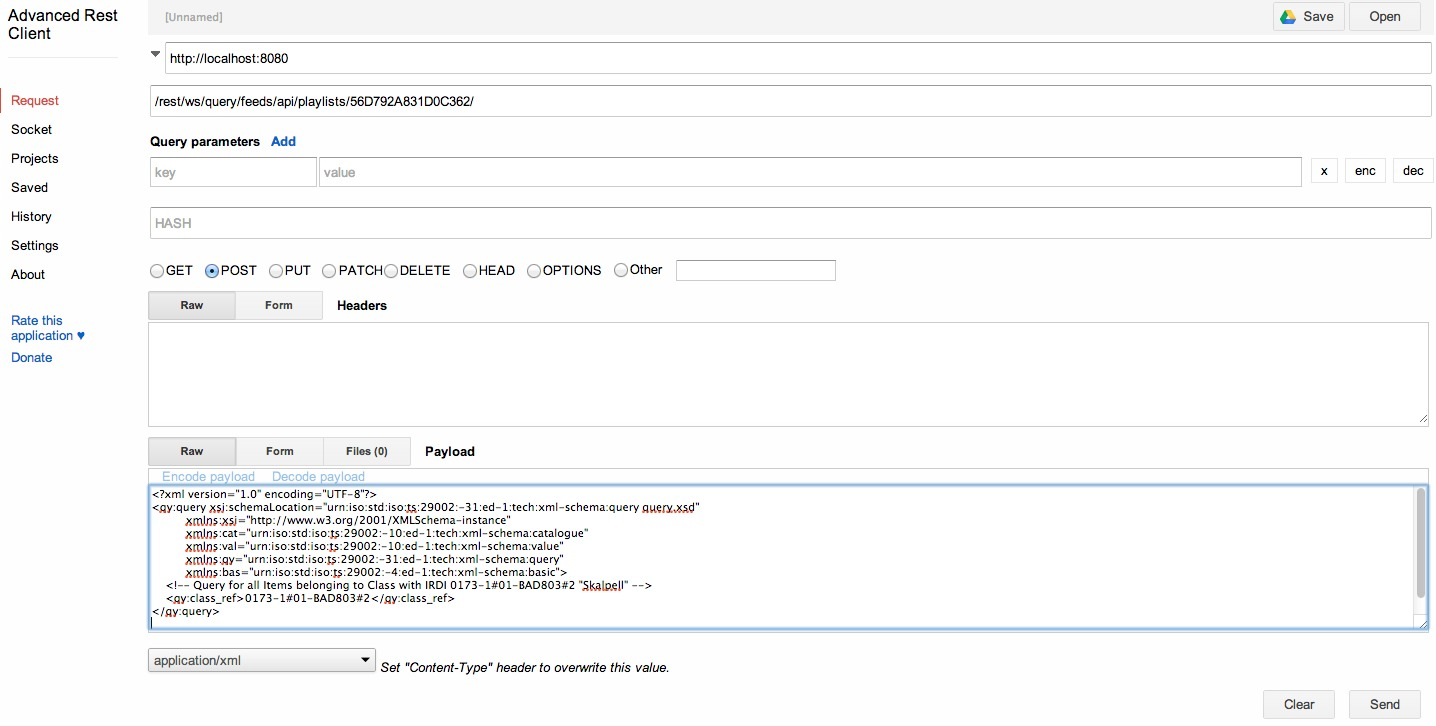
\includegraphics[width=0.98\textwidth]{images/advanced_rest_client_test.jpg}
	\caption{Advanced REST Client Test des Webservices}
	\label{fig:advancedrestclienttest}
\end{figure}


\chapter{PLIB Datenbanktabellen - Ausschnitt}\label{kap:anh_plib_db}

\autoref{fig:plib_db_tabellen} zeigt einen Ausschnitt der Datenbanktabellen. Die Abbildung wurden von Herrn Karsten Mende zur Verfügung gestellt. 

\begin{figure}[htbp]
	\centering
		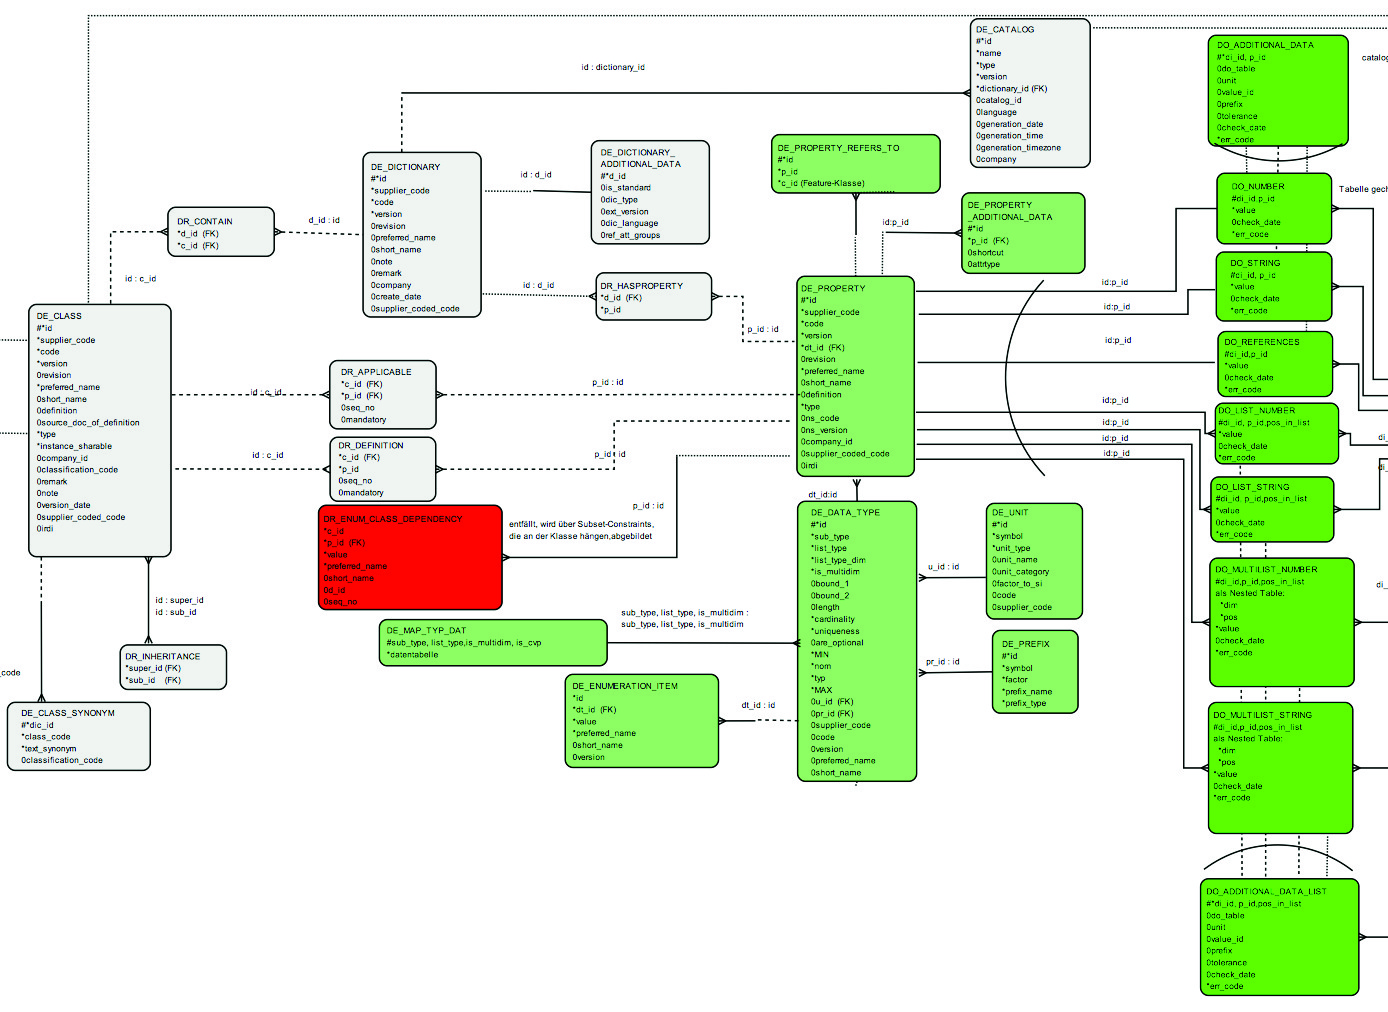
\includegraphics[width=0.98\textwidth]{images/plib_datenbankausschnitt.jpg}
	\caption{PLIB Datenbanktabellen - Ausschnitt}
	\label{fig:plib_db_tabellen}
\end{figure}
\chapter{SOAP Webservice} \index{Webservice!SOAP}\label{kap:anhang_soap_webservice}

Um die beiden unterschiedlichen Webservicearten vergleichen zu können wurde evaluiert, wie mit der gleichen Plattform, Programmiersprache und Schemadateien ein SOAP \gls{Webservice} implementiert werden kann. 

Genutzt wurde der in der Java-JDK beinhaltete Implementierung der JAX-WS-2.1-Spezifikation, somit muss keine weitere Bibliothek eingebunden werden. 

Die gesamte Business-Logik-Implementierung für den REST-Webservice kann genutzt werden. Für die Erstellung des Webservices sind folgende Schritte notwendig:

\begin{itemize}
\item Erstellung einer Webservice Klasse, welche die Business Logik aufruft
\item Erstellung eines Webservice Servers, welche den Webservice bereitstellt
\end{itemize}

\section{Erstellung einer Webservice Klasse}

Das \autoref{lst:soap_webservice_send_query} zeigt die Implementierung einer Webservice-Klasse. 

Hierbei definiert @WebService diese Klasse mittels Annotation als Webservice gemäß JAX-WS Spezifikation. 
@SOAPBinding(style=SOAPBinding.Style.DOCUMENT) definiert ein SOAP-Binding als Dokumenten Typ. Ein weiterer Typ ist RPC.
@WebMethod definiert die markierte Methode als Webservice Methode. 

Die Methode leitet den übergebenen query einfach an die Business Logik, der QueryPipe, zur weiteren Verarbeitung. Dies entspricht exakt dem Vorgehen in der query-Methode im REST-Webservice.  

\begin{lstlisting}[caption=SOAP Webservice Klasse zum Senden eines Queries, language=Java, label=lst:soap_webservice_send_query]
package de.feu.plib.webservice;

import de.feu.plib.processor.QueryPipe;
import de.feu.plib.xml.catalogue.CatalogueType;
import de.feu.plib.xml.query.QueryType;
import org.springframework.context.ApplicationContext;
import org.springframework.context.support.ClassPathXmlApplicationContext;

import javax.jws.WebMethod;
import javax.jws.WebService;
import javax.jws.soap.SOAPBinding;

/**
 * SOAP Webservice for querying via ISO 29002-31 Schema
 */
@WebService
@SOAPBinding(style=SOAPBinding.Style.DOCUMENT)
public class QuerySOAPService {

    /** Query processor instance */
    private QueryPipe queryPipe;

    /** Application context for receiving beans */
    private ApplicationContext context;

    public QuerySOAPService() {
        this.context = initializeContext();
        this.queryPipe = getQueryPipe();
    }

    /**
     * Takes the query model and passes it to the query filter for further processing.
     * Retreives the result and returns it.
     * @param query the query
     * @return the catalogue response
     */
    @WebMethod
    public CatalogueType query(QueryType query) {
        CatalogueType catalogue = queryPipe.filter(query);
        return catalogue;
    }

    private ClassPathXmlApplicationContext initializeContext() {
        return new ClassPathXmlApplicationContext(
                "beans.xml");
    }

    private QueryPipe getQueryPipe() {
        QueryPipe queryPipe =  (QueryPipe) context.getBean("queryPipe");
        return queryPipe;
    }
}
 \end{lstlisting}  
 
\section{Erstellung eines Webservice Servers}

Das \autoref{lst:soap_webservice_server} zeigt die Implementierung eines beispielhaften Webservice server. Dieser erzeugt eine Instanz der Klasse QuerySOAPService, der Klasse welche die Methoden für den Webservice beinhalten. Anschließend wird ein Endpoint definiert. Hier wird die spätere \gls{URL}, unter dem der Webservice zur Verfügung gestellt wird, definiert und der QuerySOAPService übergeben. 

Ferner wird zu Testzwecken, zum stoppen des Services, ein Dialog-Fenster angezeigt.
 
\begin{lstlisting}[caption=SOAP Webservice Server, language=Java, label=lst:soap_webservice_server]
package de.feu.plib.webservice;

import org.apache.log4j.Logger;

import javax.swing.*;
import javax.xml.ws.Endpoint;

/**
 * Is responsible for creating the SOAP Webserver.
 */
public class QueryServer {
    /** Logger instance */
    static final Logger LOGGER = Logger.getLogger(StringServer.class);

    public static void main(String args[]) {
        LOGGER.info("Start query web service");
        QuerySOAPService queryService = new QuerySOAPService();
        Endpoint endpoint = Endpoint.publish(
                "http://localhost:8088/soap/query", queryService);
        LOGGER.info("Web service started");
        JOptionPane.showMessageDialog(null, "Server beenden");
        endpoint.stop();
        LOGGER.info("Web service started");
    }
}
 \end{lstlisting}   

\section{SOAP Beispielrequest und -response}

Das \autoref{lst:soap_query} zeigt einen Beispielrequest und \autoref{lst:soap_response} zeigt die entsprechende Antwort des Servers. 

\begin{lstlisting}[caption=Beispielanfrage SOAP Webservice query, language=XML, label=lst:soap_query]
 <soapenv:Envelope xmlns:soapenv="http://schemas.xmlsoap.org/soap/envelope/" xmlns:web="http://webservice.plib.feu.de/" xmlns:urn="urn:iso:std:iso:ts:29002:-31:ed-1:tech:xml-schema:query" xmlns:urn1="urn:iso:std:iso:ts:29002:-10:ed-1:tech:xml-schema:catalogue" xmlns:urn2="urn:iso:std:iso:ts:29002:-4:ed-1:tech:xml-schema:basic" xmlns:urn3="urn:iso:std:iso:ts:29002:-10:ed-1:tech:xml-schema:value">
   <soapenv:Header/>
   <soapenv:Body>
      <web:query>
         <arg0>
            <urn:class_ref>0173-1#01-BAD803#2</urn:class_ref>
	 </arg0>
      </web:query>
   </soapenv:Body>
</soapenv:Envelope>    
 \end{lstlisting}  


 \begin{lstlisting}[caption=Beispielantwort SOAP Webservice response, language=XML, label=lst:soap_response]
<S:Envelope xmlns:S="http://schemas.xmlsoap.org/soap/envelope/">
   <S:Body>
      <ns6:queryResponse xmlns:ns2="urn:iso:std:iso:ts:29002:-10:ed-1:tech:xml-schema:catalogue" xmlns:ns3="urn:iso:std:iso:ts:29002:-4:ed-1:tech:xml-schema:basic" xmlns:ns4="urn:iso:std:iso:ts:29002:-10:ed-1:tech:xml-schema:value" xmlns:ns5="urn:iso:std:iso:ts:29002:-31:ed-1:tech:xml-schema:query" xmlns:ns6="http://webservice.plib.feu.de/">
         <return>
            <ns2:item class_ref="0173-1#01-BAD803#2">
               <ns2:property_value property_ref="0173-1#02-AAA762#1">
                  <ns4:measure_single_number_value>
                     <ns4:real_value>2.0</ns4:real_value>
                  </ns4:measure_single_number_value>
               </ns2:property_value>
               <ns2:property_value property_ref="0173-1#02-AAB011#1">
                  <ns4:measure_single_number_value>
                     <ns4:real_value>1.0</ns4:real_value>
                  </ns4:measure_single_number_value>
               </ns2:property_value>
            </ns2:item>
            <ns2:item class_ref="0173-1#01-BAD803#2">
               <ns2:property_value property_ref="0173-1#02-AAA762#1">
                  <ns4:measure_single_number_value>
                     <ns4:real_value>2.0</ns4:real_value>
                  </ns4:measure_single_number_value>
               </ns2:property_value>
               <ns2:property_value property_ref="0173-1#02-AAB011#1">
                  <ns4:measure_single_number_value>
                     <ns4:real_value>1.0</ns4:real_value>
                  </ns4:measure_single_number_value>
               </ns2:property_value>
            </ns2:item>
         </return>
      </ns6:queryResponse>
   </S:Body>
</S:Envelope>  
 \end{lstlisting}  
 
 Die \autoref{lst:wsdl_query_service} zeigt die WSDL des Query Services. Diese wurde automatisch generiert. Das geschieht durch den Aufruf der URL des Services mit Query-Parameter ?wsdl. 
 
 Folgende URL wurde aufgerufen: http://localhost:8088/soap/query?wsdl
 
 Man sieht, dass die benötigten Schemadateien für query, basic, value und catalogue der ISO XSDs automatisch eingebunden werden. Der Grund ist, dass in den Java Sourcen wie in \autoref{lst:soap_webservice_send_query} ersichtlich, die bereits während der REST-Implementierung für das Marshalling und Unmarshalling erzeugten Zugriffsklassen mittels JAXB benutzt werden. Das sind CatalogueType und QueryType. Dies sind JAXB annotierte Klassen, somit werden automatisch die entsprechenden Schemadateien verwendet.
 
 \begin{lstlisting}[caption=WSDL des Query Services mit SOAP, language=XML, label=lst:wsdl_query_service] 
 <!--
 Published by JAX-WS RI at http://jax-ws.dev.java.net. RI's version is JAX-WS RI 2.1.6 in JDK 6.
-->
<!--
 Generated by JAX-WS RI at http://jax-ws.dev.java.net. RI's version is JAX-WS RI 2.1.6 in JDK 6.
-->
<definitions xmlns:soap="http://schemas.xmlsoap.org/wsdl/soap/" xmlns:tns="http://webservice.plib.feu.de/"
             xmlns:xsd="http://www.w3.org/2001/XMLSchema" xmlns="http://schemas.xmlsoap.org/wsdl/"
             targetNamespace="http://webservice.plib.feu.de/" name="QuerySOAPServiceService">
    <types>
        <xsd:schema>
            <xsd:import namespace="urn:iso:std:iso:ts:29002:-4:ed-1:tech:xml-schema:basic"
                        schemaLocation="http://localhost:8088/soap/query?xsd=1"/>
        </xsd:schema>
        <xsd:schema>
            <xsd:import namespace="urn:iso:std:iso:ts:29002:-31:ed-1:tech:xml-schema:query"
                        schemaLocation="http://localhost:8088/soap/query?xsd=2"/>
        </xsd:schema>
        <xsd:schema>
            <xsd:import namespace="urn:iso:std:iso:ts:29002:-10:ed-1:tech:xml-schema:value"
                        schemaLocation="http://localhost:8088/soap/query?xsd=3"/>
        </xsd:schema>
        <xsd:schema>
            <xsd:import namespace="urn:iso:std:iso:ts:29002:-10:ed-1:tech:xml-schema:catalogue"
                        schemaLocation="http://localhost:8088/soap/query?xsd=4"/>
        </xsd:schema>
        <xsd:schema>
            <xsd:import namespace="http://webservice.plib.feu.de/"
                        schemaLocation="http://localhost:8088/soap/query?xsd=5"/>
        </xsd:schema>
    </types>
    <message name="query">
        <part name="parameters" element="tns:query"/>
    </message>
    <message name="queryResponse">
        <part name="parameters" element="tns:queryResponse"/>
    </message>
    <portType name="QuerySOAPService">
        <operation name="query">
            <input message="tns:query"/>
            <output message="tns:queryResponse"/>
        </operation>
    </portType>
    <binding name="QuerySOAPServicePortBinding" type="tns:QuerySOAPService">
        <soap:binding transport="http://schemas.xmlsoap.org/soap/http" style="document"/>
        <operation name="query">
            <soap:operation soapAction=""/>
            <input>
                <soap:body use="literal"/>
            </input>
            <output>
                <soap:body use="literal"/>
            </output>
        </operation>
    </binding>
    <service name="QuerySOAPServiceService">
        <port name="QuerySOAPServicePort" binding="tns:QuerySOAPServicePortBinding">
            <soap:address location="http://localhost:8088/soap/query"/>
        </port>
    </service>
</definitions>
  \end{lstlisting} 
 
 \section{Fazit}
 
Da sämtliche Voraussetzungen bereits während der Implementierung des REST-Webservices in der Business Logik vorhanden waren, konnte in kurzer Zeit ein SOAP-Webservice erstellt werden, der die gleichen Query-Funktionalitäten zur Verfügung stellt wie der REST-Webservice. Das Generieren des XML-Modells in Java-Klassen wurde bereits mittels JAXB durchgeführt, sodass diese Modelle erneut benutzt werden können. Java kennt dann die Modelle und die Bindung an die entsprechenden XML-Schema-Dateien, so dass diese für den \gls{Webservice} zur Verfügung gestellt werden können. 
Es ist also ersichtlich, dass die Webservice Schnittstelle mit relativ geringem Aufwand ausgetauscht werden kann, wenn die Business Logik gekapselt wurde. 
\chapter{Architektur - Bausteinsichten} \label{kap:anh_architektur}

Dieses Kapitel enthält weiter verfeinerte Bausteinansichten über das System.

\section{Level 2 - Whiteboxansicht - Komponente XMLData}\index{Whiteboxansicht}

Die Komponente XMLData beinhaltet alle Datenmodelle für die beiden Hauptkonzepte \enquote{Query for characteristic data} nach. Siehe dazu \autoref{fig:bausteinsicht_level2_xmldata}. 

\begin{figure}[htbp]
	\centering
		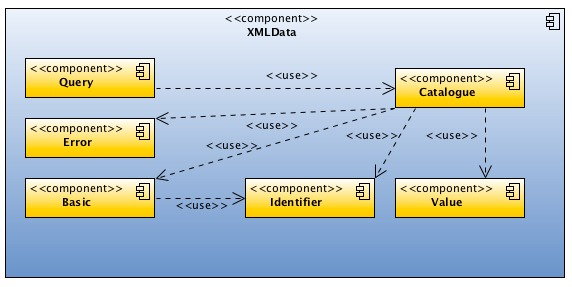
\includegraphics[width=0.82\textwidth]{images/bausteinsicht_plib_level2_xmldata.jpg}
	\caption{Bausteinsicht - Level 2 - Komponente XMLData}
	\label{fig:bausteinsicht_level2_xmldata}
\end{figure}

\begin{description}
\item[Query] Diese Komponente beinhaltet das Datenmodell des Queries nach ISO/TS 29002-31. 
\item[Catalogue] Diese Komponente beinhaltet das Datenmodell des Kataloges nach ISO/TS 29002-10. 
\item[Basic] Diese Komponente beinhaltet das Datenmodell von Basistypen nach ISO/TS 29002-4.
\item[Value] Diese Komponente beinhaltet das Datenmodell der Wertetypen nach ISO/TS 29002-10.
\item[Identifier] Diese Komponente beinhaltet das Datenmodell für Identifier (IRDI) nach ISO/TS 29002-5. 
\end{description}

\section{Level 2 - Whiteboxansicht - Komponente Processor}\index{Whiteboxansicht}

Die Komponente Processor beinhaltet den QueryProcessor sowie die Handler und Analyser-Komponente. Siehe dazu \autoref{fig:bausteinsicht_level2_processor}. 

\begin{figure}[htbp]
	\centering
		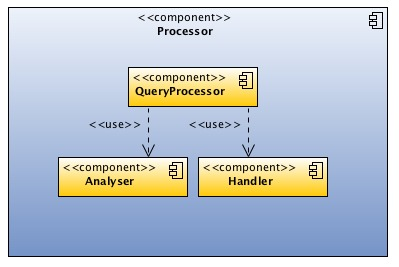
\includegraphics[width=0.70\textwidth]{images/bausteinsicht_plib_level2_processor.jpg}
	\caption{Bausteinsicht - Level 2 - Komponente Processor}
	\label{fig:bausteinsicht_level2_processor}
\end{figure}

\begin{description}
\item[QueryProcessor] Diese Komponente ist für die erste Queryverarbeitung verantwortlich. Übernimmt eine Erkennung des Queries und leitet an den Handler und Analyser weiter. 
\item[Handler] Diese Komponente beinhaltet die QueryServices, welche die eigentliche Verarbeitung und Transformation der Queries in die Datenmodelle übernimmt.
\item[Analyser] Enthält Komponenten zur Analyse und Markierung des Queries für die weitere Verarbeitung. 
\end{description}

\section{Level 3 - Whiteboxansicht - Komponente Handler}\index{Whiteboxansicht}

Die Komponente Handler beinhaltet die QueryServices, die zur Verarbeitung sowie Transformation der Queries zuständig sind. Siehe dazu \autoref{fig:bausteinsicht_level3_handler}. 

\begin{figure}[htbp]
	\centering
		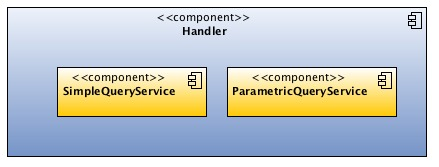
\includegraphics[width=0.82\textwidth]{images/bausteinsicht_plib_level3_handler.jpg}
	\caption{Bausteinsicht - Level 3 - Komponente Handler}
	\label{fig:bausteinsicht_level3_handler}
\end{figure}

\begin{description}
\item[SimpleQueryService] Diese Komponente ist für die Verarbeitung und Transformation der SimpleQueries (Projektion) zuständig. Bereitet die Anfrage für die Datenbank für die PLIBDao-Komponente vor. 
\item[ParametricQueryService] Diese Komponente ist für die Verarbeitung und Transformation der ParametricQueries (Selektion) zuständig. Bereitet die Anfrage für die Datenbank für die PLIBDao-Komponente vor. 
\end{description}

\section{Level 3 - Whiteboxansicht - Komponente Analyser}\index{Whiteboxansicht}

Die Komponente Analyser beinhaltet Komponenten zur Analyse und Markieren der Eingangsqueries. Siehe dazu \autoref{fig:bausteinsicht_level3_analyser}. 

\begin{figure}[htbp]
	\centering
		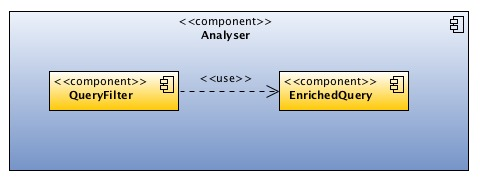
\includegraphics[width=0.82\textwidth]{images/bausteinsicht_plib_level3_analyser.jpg}
	\caption{Bausteinsicht - Level 3 - Komponente Analyser}
	\label{fig:bausteinsicht_level3_analyser}
\end{figure}

\begin{description}
\item[QueryFilter] Diese Komponente filtert den Eingangsquery und markiert ihn mit Hilfe von EnrichedQuery.
\item[EnrichedQuery] Diese Komponente markiert den Query gemäß seiner Art (Simple, Parametric), zur späteren schnellen Erkennung. Es muss somit keine aufwändige Erkennung durch prüfen der Eingangsdaten durchgeführt werden, sondern es können Flags in dieser Komponente abgefragt werden. 
\end{description}


\chapter{Schema Dateien} \index{Schema-Dateien}\label{kap:anhang_schema}

\section{query.xsd}\index{Schema!query.xsd}

 \begin{lstlisting}[caption=query.xsd, language=XML, label=lst:query_xsd]
<?xml version="1.0" encoding="UTF-8"?>
<!--
$Id: query.xsd 411 2009-07-21 01:57:47Z radack $
ISO TC 184/SC 4/WG 12 N6664 - ISO/TS 29002-31 Query - XML schema
-->
<!--
The following permission notice and disclaimer shall be included in all copies of this XML schema ("the Schema"), and derivations of the Schema:

Permission is hereby granted, free of charge in perpetuity, to any person obtaining a copy of the Schema, to use, copy, modify, merge and distribute free of charge, copies of the Schema for the purposes of developing, implementing, installing and using software based on the  Schema, and to permit persons to whom the Schema is furnished to do so, subject to the following conditions:

THE SCHEMA IS PROVIDED "AS IS", WITHOUT WARRANTY OF ANY KIND, EXPRESS OR IMPLIED, INCLUDING BUT NOT LIMITED TO THE WARRANTIES OF MERCHANTABILITY, FITNESS FOR A PARTICULAR PURPOSE AND NONINFRINGEMENT. IN NO EVENT SHALL THE AUTHORS OR COPYRIGHT HOLDERS BE LIABLE FOR ANY CLAIM, DAMAGES OR OTHER LIABILITY, WHETHER IN AN ACTION OF CONTRACT, TORT OR OTHERWISE, ARISING FROM, OUT OF OR IN CONNECTION WITH THE SCHEMA OR THE USE OR OTHER DEALINGS IN THE SCHEMA.

In addition, any modified copy of the Schema shall include the following notice:

THIS SCHEMA HAS BEEN MODIFIED FROM THE SCHEMA DEFINED IN ISO 29002-31, AND SHOULD NOT BE INTERPRETED AS COMPLYING WITH THAT STANDARD.

-->
<xs:schema xmlns:xs="http://www.w3.org/2001/XMLSchema"
           xmlns:qy="urn:iso:std:iso:ts:29002:-31:ed-1:tech:xml-schema:query"
           xmlns:cat="urn:iso:std:iso:ts:29002:-10:ed-1:tech:xml-schema:catalogue"
           xmlns:val="urn:iso:std:iso:ts:29002:-10:ed-1:tech:xml-schema:value"
           xmlns:bas="urn:iso:std:iso:ts:29002:-4:ed-1:tech:xml-schema:basic"
           xmlns:id="urn:iso:std:iso:ts:29002:-5:ed-1:tech:xml-schema:identifier"
           targetNamespace="urn:iso:std:iso:ts:29002:-31:ed-1:tech:xml-schema:query" elementFormDefault="qualified">
    <xs:import namespace="urn:iso:std:iso:ts:29002:-4:ed-1:tech:xml-schema:basic" schemaLocation="basic.xsd"/>
    <xs:import namespace="urn:iso:std:iso:ts:29002:-5:ed-1:tech:xml-schema:identifier" schemaLocation="identifier.xsd"/>
    <xs:import namespace="urn:iso:std:iso:ts:29002:-10:ed-1:tech:xml-schema:catalogue" schemaLocation="catalogue.xsd"/>
    <xs:import namespace="urn:iso:std:iso:ts:29002:-10:ed-1:tech:xml-schema:value" schemaLocation="value.xsd"/>
    <!-- Global Elements -->
    <xs:element name="characteristic_data_query_expression" type="qy:characteristic_data_query_expression_Type"/>
    <xs:element name="query" type="qy:query_Type"/>
    <xs:element name="query_context" type="qy:query_context_Type"/>
    <!-- Global Types -->
    <!-- Characteristic Data Query Expression -->
    <xs:complexType name="characteristic_data_query_expression_Type">
        <xs:choice>
            <xs:element name="cardinality" type="qy:cardinality_expression_Type"/>
            <xs:element name="range" type="qy:range_expression_Type"/>
            <xs:element name="string_pattern" type="qy:string_pattern_expression_Type"/>
            <xs:element name="string_size" type="qy:string_size_expression_Type"/>
            <xs:element name="subset" type="qy:subset_expression_Type"/>
            <xs:element name="data_environment" type="qy:data_environment_expression_Type"/>
            <xs:element name="or" type="qy:or_expression_Type"/>
            <xs:element name="and" type="qy:and_expression_Type"/>
            <xs:element name="not" type="qy:not_expression_Type"/>
        </xs:choice>
    </xs:complexType>
    <!-- Or Expression -->
    <xs:complexType name="or_expression_Type">
        <xs:sequence>
            <xs:element name="operand" type="qy:characteristic_data_query_expression_Type" minOccurs="2"
                        maxOccurs="unbounded"/>
        </xs:sequence>
    </xs:complexType>
    <!-- And query expression -->
    <xs:complexType name="and_expression_Type">
        <xs:sequence>
            <xs:element name="operand" type="qy:characteristic_data_query_expression_Type" minOccurs="2"
                        maxOccurs="unbounded"/>
        </xs:sequence>
    </xs:complexType>
    <!-- Not Expression -->
    <xs:complexType name="not_expression_Type">
        <xs:sequence>
            <xs:element name="operand" type="qy:characteristic_data_query_expression_Type"/>
        </xs:sequence>
    </xs:complexType>
    <!-- -->
    <!-- Query Expression -->
    <xs:complexType name="query_expression_Type" abstract="true">
        <xs:sequence>
            <xs:element name="property_reference" type="qy:property_reference_Type"/>
        </xs:sequence>
    </xs:complexType>
    <!-- Cardinality Expression -->
    <xs:complexType name="cardinality_expression_Type">
        <xs:complexContent>
            <xs:extension base="qy:query_expression_Type">
                <xs:sequence>
                    <xs:element name="minimum" type="xs:int" minOccurs="0"/>
                    <xs:element name="maximum" type="xs:int" minOccurs="0"/>
                </xs:sequence>
            </xs:extension>
        </xs:complexContent>
    </xs:complexType>
    <!-- Range Expression -->
    <xs:complexType name="range_expression_Type">
        <xs:complexContent>
            <xs:extension base="qy:query_expression_Type">
                <xs:sequence>
                    <xs:element name="min_value" type="xs:float" minOccurs="0"/>
                    <xs:element name="max_value" type="xs:float" minOccurs="0"/>
                    <xs:element name="UOM_ref" type="id:IRDI_type" minOccurs="0"/>
                    <xs:element name="UOM_code" type="xs:string" minOccurs="0"/>
                    <xs:element name="currency_ref" type="id:IRDI_type" minOccurs="0"/>
                    <xs:element name="currency_code" type="bas:ISO_currency_code_Type" minOccurs="0"/>
                    <xs:element name="is_inclusive" type="xs:boolean"/>
                </xs:sequence>
            </xs:extension>
        </xs:complexContent>
    </xs:complexType>
    <!-- String Pattern Expression -->
    <xs:complexType name="string_pattern_expression_Type">
        <xs:complexContent>
            <xs:extension base="qy:query_expression_Type">
                <xs:sequence>
                    <xs:element name="pattern" type="xs:string"/>
                    <xs:element name="language_ref" type="id:IRDI_type" minOccurs="0"/>
                    <xs:element name="language_code" type="bas:ISO_language_code_Type" minOccurs="0"/>
                    <xs:element name="country_code" type="bas:ISO_country_code_Type" minOccurs="0"/>
                </xs:sequence>
            </xs:extension>
        </xs:complexContent>
    </xs:complexType>
    <!-- String Size Expression -->
    <xs:complexType name="string_size_expression_Type">
        <xs:complexContent>
            <xs:extension base="qy:query_expression_Type">
                <xs:sequence>
                    <xs:element name="min_length" type="xs:int" minOccurs="0"/>
                    <xs:element name="max_length" type="xs:int" minOccurs="0"/>
                    <xs:element name="language_ref" type="id:IRDI_type" minOccurs="0"/>
                    <xs:element name="language_code" type="bas:ISO_language_code_Type" minOccurs="0"/>
                    <xs:element name="country_code" type="bas:ISO_country_code_Type" minOccurs="0"/>
                </xs:sequence>
            </xs:extension>
        </xs:complexContent>
    </xs:complexType>
    <!-- Subset Expression -->
    <xs:complexType name="subset_expression_Type">
        <xs:complexContent>
            <xs:extension base="qy:query_expression_Type">
                <xs:sequence>
                    <xs:element name="value" type="qy:value_Type" minOccurs="0" maxOccurs="unbounded"/>
                </xs:sequence>
            </xs:extension>
        </xs:complexContent>
    </xs:complexType>
    <!-- Value -->
    <xs:complexType name="value_Type">
        <xs:sequence>
            <xs:group ref="val:value_Group"/>
        </xs:sequence>
    </xs:complexType>
    <!-- Data Environment Expression -->
    <xs:complexType name="data_environment_expression_Type">
        <xs:complexContent>
            <xs:extension base="qy:query_expression_Type">
                <xs:sequence>
                    <xs:element name="environment" type="qy:characteristic_data_query_expression_Type"
                                maxOccurs="unbounded"/>
                </xs:sequence>
            </xs:extension>
        </xs:complexContent>
    </xs:complexType>
    <!-- -->
    <!-- Property Reference -->
    <xs:complexType name="property_reference_Type">
        <xs:sequence>
            <xs:element name="index" type="xs:int" minOccurs="0"/>
            <xs:element name="property" type="qy:property_reference_Type" minOccurs="0"/>
        </xs:sequence>
        <xs:attribute name="property_ref" type="id:IRDI_type" use="required"/>
    </xs:complexType>
    <!-- Query -->
    <xs:complexType name="query_Type">
        <xs:sequence>
            <xs:element name="item_description" type="xs:string" minOccurs="0"/>
            <xs:element name="data_specification_ref" type="id:IRDI_type" minOccurs="0"/>
            <xs:element name="class_ref" type="id:IRDI_type" minOccurs="0"/>
            <xs:element name="property_ref" type="id:IRDI_list_type" minOccurs="0"/>
            <xs:element ref="cat:item" minOccurs="0"/>
            <xs:element ref="qy:characteristic_data_query_expression" minOccurs="0" maxOccurs="unbounded"/>
        </xs:sequence>
    </xs:complexType>
    <!-- Query Context -->
    <xs:complexType name="query_context_Type">
        <xs:sequence>
            <xs:element name="requesting_organization_ref" type="id:IRDI_type"/>
            <xs:element name="request_date_time" type="xs:dateTime"/>
            <xs:element name="response_due_date_time" type="xs:dateTime" minOccurs="0"/>
            <xs:element name="response_email_address" type="xs:string"/>
            <xs:element name="point_of_contact" type="xs:string" minOccurs="0"/>
            <xs:element ref="qy:query" minOccurs="0" maxOccurs="unbounded"/>
        </xs:sequence>
    </xs:complexType>
</xs:schema>

 \end{lstlisting}  

\section{catalogue.xsd}\index{Schema!catalogue.xsd}

 \begin{lstlisting}[caption=catalogue.xsd, language=XML, label=lst:catalogue_xsd]
<?xml version="1.0" encoding="UTF-8"?>
<!--
$Id: catalogue.xsd 332 2009-05-29 02:16:28Z radack $
ISO TC 184/SC 4/WG 12 N5178 - ISO/TS 29002-10 Catalogue - XML schema
-->
<!--
The following permission notice and disclaimer shall be included in all copies of this XML schema ("the Schema"), and derivations of the Schema:

Permission is hereby granted, free of charge in perpetuity, to any person obtaining a copy of the Schema, to use, copy, modify, merge and distribute free of charge, copies of the Schema for the purposes of developing, implementing, installing and using software based on the  Schema, and to permit persons to whom the Schema is furnished to do so, subject to the following conditions:

THE SCHEMA IS PROVIDED "AS IS", WITHOUT WARRANTY OF ANY KIND, EXPRESS OR IMPLIED, INCLUDING BUT NOT LIMITED TO THE WARRANTIES OF MERCHANTABILITY, FITNESS FOR A PARTICULAR PURPOSE AND NONINFRINGEMENT. IN NO EVENT SHALL THE AUTHORS OR COPYRIGHT HOLDERS BE LIABLE FOR ANY CLAIM, DAMAGES OR OTHER LIABILITY, WHETHER IN AN ACTION OF CONTRACT, TORT OR OTHERWISE, ARISING FROM, OUT OF OR IN CONNECTION WITH THE SCHEMA OR THE USE OR OTHER DEALINGS IN THE SCHEMA.

In addition, any modified copy of the Schema shall include the following notice:

THIS SCHEMA HAS BEEN MODIFIED FROM THE SCHEMA DEFINED IN ISO/TS 29002-10, AND SHOULD NOT BE INTERPRETED AS COMPLYING WITH THAT STANDARD.

-->
<xs:schema xmlns:xs="http://www.w3.org/2001/XMLSchema" xmlns:cat="urn:iso:std:iso:ts:29002:-10:ed-1:tech:xml-schema:catalogue" xmlns:val="urn:iso:std:iso:ts:29002:-10:ed-1:tech:xml-schema:value" xmlns:bas="urn:iso:std:iso:ts:29002:-4:ed-1:tech:xml-schema:basic" xmlns:id="urn:iso:std:iso:ts:29002:-5:ed-1:tech:xml-schema:identifier" targetNamespace="urn:iso:std:iso:ts:29002:-10:ed-1:tech:xml-schema:catalogue" elementFormDefault="qualified">
	<xs:import namespace="urn:iso:std:iso:ts:29002:-5:ed-1:tech:xml-schema:identifier" schemaLocation="identifier.xsd"/>
	<xs:import namespace="urn:iso:std:iso:ts:29002:-4:ed-1:tech:xml-schema:basic" schemaLocation="basic.xsd"/>
	<xs:import namespace="urn:iso:std:iso:ts:29002:-10:ed-1:tech:xml-schema:value" schemaLocation="value.xsd"/>
	<!-- Global Elements -->
	<xs:element name="catalogue" type="cat:catalogue_Type"/>
	<xs:element name="item" type="cat:item_Type"/>
	<xs:element name="property_value" type="cat:property_value_Type"/>
	<xs:element name="reference" type="cat:reference_Type"/>
	<!-- Global Types -->
	<!-- Catalogue -->
	<xs:complexType name="catalogue_Type">
		<xs:sequence>
			<xs:element ref="cat:item" minOccurs="0" maxOccurs="unbounded"/>
		</xs:sequence>
	</xs:complexType>
	<!-- Item -->
	<xs:complexType name="item_Type">
		<xs:sequence>
			<xs:element name="classification_ref" type="id:IRDI_type" minOccurs="0" maxOccurs="unbounded"/>
			<xs:element ref="cat:reference" minOccurs="0" maxOccurs="unbounded"/>
			<xs:element ref="cat:property_value" minOccurs="0" maxOccurs="unbounded"/>
		</xs:sequence>
		<xs:attribute name="class_ref" type="id:IRDI_type" use="required"/>
		<xs:attribute name="data_specification_ref" type="id:IRDI_type" use="optional"/>
		<xs:attribute name="local_id" type="xs:ID" use="optional"/>
		<xs:attribute name="information_supplier_reference_string" type="xs:string" use="optional"/>
		<xs:attribute name="is_proprietary" type="xs:boolean" use="optional"/>
		<xs:attribute name="is_dependent" type="xs:boolean" use="optional"/>
		<xs:attribute name="is_global_id" type="xs:boolean" use="optional"/>
		<xs:attribute name="is_model" type="xs:boolean" use="optional"/>
		<xs:attribute name="created_view" type="id:IRDI_type" use="optional"/>
		<xs:attribute name="view_of" type="xs:IDREF" use="optional"/>
	</xs:complexType>
	<!-- Property Value -->
	<xs:complexType name="property_value_Type">
		<xs:sequence>
			<xs:group ref="val:extended_value_Group"/>
			<xs:element ref="val:environment" minOccurs="0"/>
		</xs:sequence>
		<xs:attribute name="property_ref" type="id:IRDI_type" use="required"/>
		<xs:attribute name="subitem_path_property_ref" type="id:IRDI_list_type" use="optional"/>
		<xs:attribute name="is_proprietary" type="xs:boolean" use="optional"/>
	</xs:complexType>
	<!-- Reference -->
	<xs:complexType name="reference_Type">
		<xs:sequence>
			<xs:element name="designation" type="bas:international_text_Type" minOccurs="0"/>
		</xs:sequence>
		<xs:attribute name="organization_ref" type="id:IRDI_type" use="optional"/>
		<xs:attribute name="organization_code" type="xs:string" use="optional"/>
		<!-- Constraint: organization_ref or organization_code (or both) must be specified. -->
		<!-- Constraint: If both organization_ref and organization_code are specified, they must denote the same organization. -->
		<xs:attribute name="reference_number" type="xs:string" use="required"/>
	</xs:complexType>
</xs:schema>

 \end{lstlisting} 
 
 \section{basic.xsd}\index{Schema!basic.xsd}

 \begin{lstlisting}[caption=basic.xsd, language=XML, label=lst:basic_xsd]
<?xml version="1.0" encoding="UTF-8"?>
<!--
$Id: basic.xsd 411 2009-07-21 01:57:47Z radack $
ISO TC 184/SC 4/WG 12 N6650 - ISO/TS 29002-4 Basic - XML schema
-->
<!--
The following permission notice and disclaimer shall be included in all copies of this XML schema ("the Schema"), and derivations of the Schema:

Permission is hereby granted, free of charge in perpetuity, to any person obtaining a copy of the Schema, to use, copy, modify, merge and distribute free of charge, copies of the Schema for the purposes of developing, implementing, installing and using software based on the  Schema, and to permit persons to whom the Schema is furnished to do so, subject to the following conditions:

THE SCHEMA IS PROVIDED "AS IS", WITHOUT WARRANTY OF ANY KIND, EXPRESS OR IMPLIED, INCLUDING BUT NOT LIMITED TO THE WARRANTIES OF MERCHANTABILITY, FITNESS FOR A PARTICULAR PURPOSE AND NONINFRINGEMENT. IN NO EVENT SHALL THE AUTHORS OR COPYRIGHT HOLDERS BE LIABLE FOR ANY CLAIM, DAMAGES OR OTHER LIABILITY, WHETHER IN AN ACTION OF CONTRACT, TORT OR OTHERWISE, ARISING FROM, OUT OF OR IN CONNECTION WITH THE SCHEMA OR THE USE OR OTHER DEALINGS IN THE SCHEMA.

In addition, any modified copy of the Schema shall include the following notice:

THIS SCHEMA HAS BEEN MODIFIED FROM THE SCHEMA DEFINED IN ISO/TS 29002-4, AND SHOULD NOT BE INTERPRETED AS COMPLYING WITH THAT STANDARD.

-->
<xs:schema xmlns:xs="http://www.w3.org/2001/XMLSchema" xmlns:basic="urn:iso:std:iso:ts:29002:-4:ed-1:tech:xml-schema:basic" xmlns:id="urn:iso:std:iso:ts:29002:-5:ed-1:tech:xml-schema:identifier" targetNamespace="urn:iso:std:iso:ts:29002:-4:ed-1:tech:xml-schema:basic" elementFormDefault="qualified">
	<xs:import namespace="urn:iso:std:iso:ts:29002:-5:ed-1:tech:xml-schema:identifier" schemaLocation="identifier.xsd"/>
	<!-- Global Types -->
	<!-- Day Interval -->
	<xs:simpleType name="day_interval_Type">
		<xs:union memberTypes="xs:gYear xs:gYearMonth xs:date"/>
	</xs:simpleType>
	<!-- ASN.1 Identifier -->
	<xs:simpleType name="ASN1_identifier_Type">
		<xs:restriction base="xs:string"/>
	</xs:simpleType>
	<!-- International Text -->
	<xs:complexType name="international_text_Type">
		<xs:sequence>
			<xs:element name="local_string" type="basic:language_string_Type" maxOccurs="unbounded"/>
		</xs:sequence>
	</xs:complexType>
	<!-- ISO Country Code -->
	<xs:simpleType name="ISO_country_code_Type">
		<xs:restriction base="xs:string">
			<xs:pattern value="[A-Z]{2}"/>
		</xs:restriction>
	</xs:simpleType>
	<!-- ISO Currency Code -->
	<xs:simpleType name="ISO_currency_code_Type">
		<xs:restriction base="xs:string">
			<xs:length value="3"/>
		</xs:restriction>
	</xs:simpleType>
	<!-- ISO Language Code -->
	<xs:simpleType name="ISO_language_code_Type">
		<xs:restriction base="xs:string">
			<xs:pattern value="[a-z]{2}"/>
			<xs:pattern value="[a-z]{3}"/>
		</xs:restriction>
	</xs:simpleType>
	<!-- Language String -->
	<xs:complexType name="language_string_Type">
		<xs:sequence>
			<xs:element name="content" type="xs:string"/>
			<xs:element name="language_ref" type="id:IRDI_type" minOccurs="0"/>
			<xs:sequence minOccurs="0">
				<xs:element name="language_code" type="basic:ISO_language_code_Type"/>
				<xs:element name="country_code" type="basic:ISO_country_code_Type" minOccurs="0"/>
			</xs:sequence>
			<!-- Constraint: language or language_code (or both) must be specified. -->
			<!-- Constraint: If both language and language_code are specified, then language and the combination of language_code and country_code must denote the same localized language. -->
		</xs:sequence>
	</xs:complexType>
</xs:schema>

 \end{lstlisting} 
 
\section{identifier.xsd}\index{Schema!identifier.xsd}

 \begin{lstlisting}[caption=identifier.xsd, language=XML, label=lst:identifier_xsd]
<?xml version="1.0" encoding="UTF-8"?>
<!--
$Id: identifier.xsd 420 2009-07-25 21:51:57Z radack $
ISO TC 184/SC 4/WG 12 N5180 - ISO/TS 29002-5 Identifier - XML schema
-->
<!--
The following permission notice and disclaimer shall be included in all copies of this XML schema ("the Schema"), and derivations of the Schema:

Permission is hereby granted, free of charge in perpetuity, to any person obtaining a copy of the Schema, to use, copy, modify, merge and distribute free of charge, copies of the Schema for the purposes of developing, implementing, installing and using software based on the  Schema, and to permit persons to whom the Schema is furnished to do so, subject to the following conditions:

THE SCHEMA IS PROVIDED "AS IS", WITHOUT WARRANTY OF ANY KIND, EXPRESS OR IMPLIED, INCLUDING BUT NOT LIMITED TO THE WARRANTIES OF MERCHANTABILITY, FITNESS FOR A PARTICULAR PURPOSE AND NONINFRINGEMENT. IN NO EVENT SHALL THE AUTHORS OR COPYRIGHT HOLDERS BE LIABLE FOR ANY CLAIM, DAMAGES OR OTHER LIABILITY, WHETHER IN AN ACTION OF CONTRACT, TORT OR OTHERWISE, ARISING FROM, OUT OF OR IN CONNECTION WITH THE SCHEMA OR THE USE OR OTHER DEALINGS IN THE SCHEMA.

In addition, any modified copy of the Schema shall include the following notice:

THIS SCHEMA HAS BEEN MODIFIED FROM THE SCHEMA DEFINED IN ISO/TS 29002-5, AND SHOULD NOT BE INTERPRETED AS COMPLYING WITH THAT STANDARD.

-->
<!DOCTYPE xs:schema [
	<!ENTITY % identifier.dtd SYSTEM "identifier.dtd">
	%identifier.dtd;
]>
<xs:schema xmlns:xs="http://www.w3.org/2001/XMLSchema" xmlns:id="urn:iso:std:iso:ts:29002:-5:ed-1:tech:xml-schema:identifier" targetNamespace="urn:iso:std:iso:ts:29002:-5:ed-1:tech:xml-schema:identifier" elementFormDefault="qualified" attributeFormDefault="unqualified">
	<!-- IRDI -->
	<xs:element name="IRDI" type="id:IRDI_type"/>
	<xs:element name="IRDI_list" type="id:IRDI_list_type"/>
	<xs:simpleType name="IRDI_type">
		<xs:restriction base="xs:string">
			<xs:pattern value="&irdi1;"/>
			<xs:pattern value="&irdi2;"/>
			<xs:pattern value="&irdi3;"/>
		</xs:restriction>
	</xs:simpleType>
	<!-- IRDI sequence -->
	<xs:complexType name="IRDI_sequence_type">
		<xs:sequence>
			<xs:element ref="id:IRDI" minOccurs="0" maxOccurs="unbounded"/>
		</xs:sequence>
	</xs:complexType>
	<!-- IRDI list-->
	<xs:simpleType name="IRDI_list_type">
		<xs:list itemType="id:IRDI_type"/>
	</xs:simpleType>
</xs:schema>

 \end{lstlisting} 

\section{value.xsd}\index{Schema!value.xsd}
 \begin{lstlisting}[caption=value.xsd, language=XML, label=lst:value_xsd]
<?xml version="1.0" encoding="UTF-8"?>
<!--
$Id: value.xsd 332 2009-05-29 02:16:28Z radack $
ISO TC 184/SC 4/WG 12 N5192 - ISO/TS 29002-10 Value - XML schema
-->
<!--
The following permission notice and disclaimer shall be included in all copies of this XML schema ("the Schema"), and derivations of the Schema:

Permission is hereby granted, free of charge in perpetuity, to any person obtaining a copy of the Schema, to use, copy, modify, merge and distribute free of charge, copies of the Schema for the purposes of developing, implementing, installing and using software based on the  Schema, and to permit persons to whom the Schema is furnished to do so, subject to the following conditions:

THE SCHEMA IS PROVIDED "AS IS", WITHOUT WARRANTY OF ANY KIND, EXPRESS OR IMPLIED, INCLUDING BUT NOT LIMITED TO THE WARRANTIES OF MERCHANTABILITY, FITNESS FOR A PARTICULAR PURPOSE AND NONINFRINGEMENT. IN NO EVENT SHALL THE AUTHORS OR COPYRIGHT HOLDERS BE LIABLE FOR ANY CLAIM, DAMAGES OR OTHER LIABILITY, WHETHER IN AN ACTION OF CONTRACT, TORT OR OTHERWISE, ARISING FROM, OUT OF OR IN CONNECTION WITH THE SCHEMA OR THE USE OR OTHER DEALINGS IN THE SCHEMA.

In addition, any modified copy of the Schema shall include the following notice:

THIS SCHEMA HAS BEEN MODIFIED FROM THE SCHEMA DEFINED IN ISO/TS 29002-10, AND SHOULD NOT BE INTERPRETED AS COMPLYING WITH THAT STANDARD.

-->
<xs:schema xmlns:xs="http://www.w3.org/2001/XMLSchema" xmlns:val="urn:iso:std:iso:ts:29002:-10:ed-1:tech:xml-schema:value" xmlns:bas="urn:iso:std:iso:ts:29002:-4:ed-1:tech:xml-schema:basic" xmlns:id="urn:iso:std:iso:ts:29002:-5:ed-1:tech:xml-schema:identifier" targetNamespace="urn:iso:std:iso:ts:29002:-10:ed-1:tech:xml-schema:value" elementFormDefault="qualified">
	<xs:import namespace="urn:iso:std:iso:ts:29002:-5:ed-1:tech:xml-schema:identifier" schemaLocation="identifier.xsd"/>
	<xs:import namespace="urn:iso:std:iso:ts:29002:-4:ed-1:tech:xml-schema:basic" schemaLocation="basic.xsd"/>
	<!-- Global Elements -->
	<xs:element name="combination" type="val:combination_Type"/>
	<xs:element name="bag_value" type="val:bag_value_Type"/>
	<xs:element name="boolean_value" type="val:boolean_value_Type"/>
	<xs:element name="complex_value" type="val:complex_value_Type"/>
	<xs:element name="composite_value" type="val:composite_value_Type"/>
	<xs:element name="controlled_value" type="val:controlled_value_Type"/>
	<xs:element name="currency_value" type="val:currency_value_Type"/>
	<xs:element name="date_value" type="val:date_value_Type"/>
	<xs:element name="date_time_value" type="val:date_time_value_Type"/>
	<xs:element name="environment" type="val:environment_Type"/>
	<xs:element name="file_value" type="val:file_value_Type"/>
	<xs:element name="integer_value" type="val:integer_value_Type"/>
	<xs:element name="item_reference_value" type="val:item_reference_value_Type"/>
	<xs:element name="localized_text_value" type="val:localized_text_value_Type"/>
	<xs:element name="measure_qualified_number_value" type="val:measure_qualified_number_value_Type"/>
	<xs:element name="measure_range_value" type="val:measure_range_value_Type"/>
	<xs:element name="measure_single_number_value" type="val:measure_single_number_value_Type"/>
	<xs:element name="null_value" type="val:null_value_Type"/>
	<xs:element name="one_of" type="val:one_of_Type"/>
	<xs:element name="rational_value" type="val:rational_value_Type"/>
	<xs:element name="real_value" type="val:real_value_Type"/>
	<xs:element name="sequence_value" type="val:sequence_value_Type"/>
	<xs:element name="set_value" type="val:set_value_Type"/>
	<xs:element name="string_value" type="val:string_value_Type"/>
	<xs:element name="time_value" type="val:time_value_Type"/>
	<xs:element name="year_month_value" type="val:year_month_value_Type"/>
	<xs:element name="year_value" type="val:year_value_Type"/>
	<!-- Groups -->
	<!-- Extended Value -->
	<xs:group name="extended_value_Group">
		<xs:choice>
			<xs:group ref="val:value_Group"/>
			<xs:element ref="val:one_of"/>
			<xs:element ref="val:combination"/>
		</xs:choice>
	</xs:group>
	<!-- Value -->
	<xs:group name="value_Group">
		<xs:choice>
			<!-- The first element in the following list is the one that will be created by default in some XML editors whenever a property_value is added. -->
			<xs:element ref="val:string_value"/>
			<xs:element ref="val:bag_value"/>
			<xs:element ref="val:boolean_value"/>
			<xs:element ref="val:complex_value"/>
			<xs:element ref="val:composite_value"/>
			<xs:element ref="val:controlled_value"/>
			<xs:element ref="val:currency_value"/>
			<xs:element ref="val:date_value"/>
			<xs:element ref="val:date_time_value"/>
			<xs:element ref="val:file_value"/>
			<xs:element ref="val:integer_value"/>
			<xs:element ref="val:item_reference_value"/>
			<xs:element ref="val:localized_text_value"/>
			<xs:element ref="val:measure_qualified_number_value"/>
			<xs:element ref="val:measure_range_value"/>
			<xs:element ref="val:measure_single_number_value"/>
			<xs:element ref="val:null_value"/>
			<xs:element ref="val:rational_value"/>
			<xs:element ref="val:real_value"/>
			<xs:element ref="val:sequence_value"/>
			<xs:element ref="val:set_value"/>
			<xs:element ref="val:time_value"/>
			<xs:element ref="val:year_month_value"/>
			<xs:element ref="val:year_value"/>
		</xs:choice>
	</xs:group>
	<!-- Numeric Value -->
	<xs:group name="numeric_value">
		<xs:choice>
			<!-- The first element in the following list is the one that will be created by default in some XML editors whenever a property_value is added. -->
			<xs:element ref="val:real_value"/>
			<xs:element ref="val:complex_value"/>
			<xs:element ref="val:integer_value"/>
			<xs:element ref="val:rational_value"/>
		</xs:choice>
	</xs:group>
	<!-- Global Types -->
	<!-- Bag Value -->
	<xs:complexType name="bag_value_Type">
		<xs:sequence>
			<xs:group ref="val:value_Group" minOccurs="0" maxOccurs="unbounded"/>
		</xs:sequence>
	</xs:complexType>
	<!-- Boolean Value -->
	<xs:complexType name="boolean_value_Type">
		<xs:simpleContent>
			<xs:extension base="xs:boolean"/>
		</xs:simpleContent>
	</xs:complexType>
	<!-- Combination -->
	<xs:complexType name="combination_Type">
		<xs:sequence>
			<xs:group ref="val:value_Group" maxOccurs="unbounded"/>
		</xs:sequence>
	</xs:complexType>
	<!-- Complex Value -->
	<xs:complexType name="complex_value_Type">
		<xs:sequence>
			<xs:element name="real_part" type="xs:double"/>
			<xs:element name="imaginary_part" type="xs:double"/>
		</xs:sequence>
	</xs:complexType>
	<!-- Composite Value -->
	<xs:complexType name="composite_value_Type">
		<xs:sequence>
			<xs:element name="field" type="val:field_Type" minOccurs="0" maxOccurs="unbounded"/>
		</xs:sequence>
	</xs:complexType>
	<!-- Condition Element -->
	<xs:complexType name="condition_element_Type">
		<xs:sequence>
			<xs:group ref="val:value_Group"/>
		</xs:sequence>
		<xs:attribute name="property_ref" type="id:IRDI_type" use="required"/>
	</xs:complexType>
	<!-- Controlled Value -->
	<xs:complexType name="controlled_value_Type">
		<xs:attribute name="value_ref" type="id:IRDI_type" use="optional"/>
		<xs:attribute name="value_code" type="xs:string" use="optional"/>
		<!-- Constraint: value_ref or value_code (or both) must be specified. -->
		<!-- Constraint: If both value_ref and value_code specified, they must denote the same concept. -->
	</xs:complexType>
	<!-- Currency Value -->
	<xs:complexType name="currency_value_Type">
		<xs:sequence>
			<xs:group ref="val:numeric_value"/>
		</xs:sequence>
		<xs:attribute name="currency_ref" type="id:IRDI_type" use="optional"/>
		<xs:attribute name="currency_code" type="bas:ISO_currency_code_Type" use="optional"/>
		<!-- Constraint: currency_ref or currency_code (or both) must be specified. -->
		<!-- Constraint: If both currency_ref and currency_code are specified, they must denote the same concept. -->
	</xs:complexType>
	<!-- Date Value -->
	<xs:complexType name="date_value_Type">
		<xs:simpleContent>
			<xs:extension base="xs:date"/>
		</xs:simpleContent>
	</xs:complexType>
	<!-- Date Time Value -->
	<xs:complexType name="date_time_value_Type">
		<xs:simpleContent>
			<xs:extension base="xs:dateTime"/>
		</xs:simpleContent>
	</xs:complexType>
	<!-- Environment -->
	<xs:complexType name="environment_Type">
		<xs:sequence>
			<xs:element name="property_value" type="val:condition_element_Type" maxOccurs="unbounded"/>
		</xs:sequence>
	</xs:complexType>
	<!-- Field -->
	<xs:complexType name="field_Type">
		<xs:sequence>
			<xs:group ref="val:value_Group"/>
		</xs:sequence>
		<xs:attribute name="property_ref" type="id:IRDI_type" use="optional"/>
	</xs:complexType>
	<!-- File Value -->
	<xs:complexType name="file_value_Type">
		<xs:sequence>
			<xs:element name="URI" type="xs:anyURI"/>
		</xs:sequence>
	</xs:complexType>
	<!-- Integer Value -->
	<xs:complexType name="integer_value_Type">
		<xs:simpleContent>
			<xs:extension base="xs:int"/>
		</xs:simpleContent>
	</xs:complexType>
	<!-- Item Reference Value -->
	<xs:complexType name="item_reference_value_Type">
		<xs:attribute name="item_local_ref" type="xs:IDREF" use="required"/>
	</xs:complexType>
	<!-- Localized Text Value -->
	<xs:complexType name="localized_text_value_Type">
		<xs:sequence>
			<xs:element name="content" type="bas:international_text_Type"/>
		</xs:sequence>
	</xs:complexType>
	<!-- Measure Qualified Number Value -->	
	<xs:complexType name="measure_qualified_number_value_Type">
		<xs:complexContent>
			<xs:extension base="val:measure_value_Type">
				<xs:sequence>
					<xs:element name="qualified_value" type="val:qualified_value_Type" maxOccurs="unbounded"/>	
				</xs:sequence>
			</xs:extension>
		</xs:complexContent>
	</xs:complexType>
	<!-- Measure Range Value -->
	<xs:complexType name="measure_range_value_Type">
		<xs:complexContent>
			<xs:extension base="val:measure_value_Type">
				<xs:sequence>
					<xs:element name="lower_value" type="val:numeric_value_Type"/>
					<xs:element name="upper_value" type="val:numeric_value_Type"/>
				</xs:sequence>
			</xs:extension>
		</xs:complexContent>
	</xs:complexType>
	<!-- Measure Single Number Value -->
	<xs:complexType name="measure_single_number_value_Type">
		<xs:complexContent>
			<xs:extension base="val:measure_value_Type">
				<xs:sequence>
					<xs:choice>
						<xs:group ref="val:numeric_value"/>
					</xs:choice>
				</xs:sequence>
			</xs:extension>
		</xs:complexContent>
	</xs:complexType>
	<!-- Measure Value -->
	<xs:complexType name="measure_value_Type" abstract="true">
		<xs:attribute name="UOM_ref" type="id:IRDI_type" use="optional"/>
		<xs:attribute name="UOM_code" type="xs:string" use="optional"/>
		<!-- Constraint: UOM_ref or UOM_code (or both) must be specified. -->
		<!-- Constraint: If UOM_ref or UOM_code are specified, they must denote the same concept. -->
	</xs:complexType>
	<!-- Null Value -->
	<xs:complexType name="null_value_Type"/>
	<!-- Numeric Value -->
	<xs:complexType name="numeric_value_Type">
		<xs:sequence>
			<xs:group ref="val:numeric_value"/>
		</xs:sequence>
	</xs:complexType>
	<!-- OneOf -->
	<xs:complexType name="one_of_Type">
		<xs:sequence>
			<xs:choice maxOccurs="unbounded">
				<xs:element ref="val:combination"/>
				<xs:group ref="val:value_Group"/>
			</xs:choice>
		</xs:sequence>
	</xs:complexType>
	<!-- Qualified Value -->
	<xs:complexType name="qualified_value_Type">
		<xs:sequence>
			<xs:group ref="val:numeric_value"/>
		</xs:sequence>
		<xs:attribute name="qualifier_ref" type="id:IRDI_type" use="optional"/>
		<xs:attribute name="qualifier_code" type="xs:string" use="optional"/>
		<!-- Constraint: qualifier_ref or qualifier_code (or both) must be specified. -->
		<!-- Constraint: If both qualifier_ref or qualifier_code are specified, they must denote the same concept. -->
	</xs:complexType>
	<!-- Rational Value -->
	<xs:complexType name="rational_value_Type">
		<xs:sequence>
			<xs:element name="whole_part" type="xs:int" minOccurs="0"/>
			<xs:element name="numerator" type="xs:int"/>
			<xs:element name="denominator" type="xs:int"/>
		</xs:sequence>
	</xs:complexType>
	<!-- Real Value -->
	<xs:complexType name="real_value_Type">
		<xs:simpleContent>
			<xs:extension base="xs:double"/>
		</xs:simpleContent>
	</xs:complexType>
	<!-- Sequence Value -->
	<xs:complexType name="sequence_value_Type">
		<xs:sequence>
			<xs:group ref="val:value_Group" minOccurs="0" maxOccurs="unbounded"/>
		</xs:sequence>
	</xs:complexType>
	<!-- Set Value -->
	<xs:complexType name="set_value_Type">
		<xs:sequence>
			<xs:group ref="val:value_Group" minOccurs="0" maxOccurs="unbounded"/>
		</xs:sequence>
	</xs:complexType>
	<!-- String Value -->
	<xs:complexType name="string_value_Type">
		<xs:simpleContent>
			<xs:extension base="xs:string"/>
		</xs:simpleContent>
	</xs:complexType>
	<!-- Time Value -->
	<xs:complexType name="time_value_Type">
		<xs:simpleContent>
			<xs:extension base="xs:time"/>
		</xs:simpleContent>
	</xs:complexType>
	<!-- Year Month Value -->
	<xs:complexType name="year_month_value_Type">
		<xs:simpleContent>
			<xs:extension base="xs:gYearMonth"/>
		</xs:simpleContent>
	</xs:complexType>
	<!-- Year Value -->
	<xs:complexType name="year_value_Type">
		<xs:simpleContent>
			<xs:extension base="xs:gYear"/>
		</xs:simpleContent>
	</xs:complexType>
</xs:schema>

 \end{lstlisting}  

% Index
\renewcommand{\indexname}{Index}
\addcontentsline{toc}{chapter}{Index}

%\renewcommand{\nomname}{Index}

\printindex

\end{document}

